% English HKUST CSE PhD thesis. Build with make; sources and verification in planning/.
\documentclass[customlatinfont=gyre,displaycommittee=false,blankpage=false]{template/hkust-thesis-v0.11.6/hkustthesis}
\usepackage{longtable}
\setlength{\emergencystretch}{4em}
\AtBeginBibliography{\small\sloppy}
\usepackage{pdflscape}
\usepackage[normalem]{ulem}
\hkustsetup{info={degree={phd},title={Structural Augmented Reasoning for Language Models},keywords={knowledge graphs,language models,retrieval-augmented generation},author={Yubo Wang},school={School of Engineering},department={Department of Computer Science and Engineering},program={Computer Science and Engineering},major={},supervisor={Prof. Lei Chen, Chair Professor},co-supervisor={},submit-month={December 2026},submit-date={\rule{32mm}{0.3pt}},defend-date={27 November 2026},depthead={\rule{52mm}{0.3pt}\\Head of Department},reviewer={},reviewerdept={},reviewerext={},city={Hong Kong}}}
\addbibresource{thesis-references.bib}
\newtheorem{thesisdefinition}{Definition}[chapter]
\newtheorem{thesistheorem}{Theorem}[chapter]
\begin{document}
\frontmatter
\maketitle
\begin{abstract}
Language models depend on the evidence supplied to their prediction and generation processes. Tables can omit information needed for semantic annotation, classification labels can evolve under limited supervision, and answers can require relationships distributed across textual and visual sources. This thesis investigates how explicit knowledge structures can organize and select evidence for these settings.

The thesis develops four methods for structural augmentation. KGLink integrates knowledge graphs with a pre-trained language model to enrich column representations and bridge differences between graph types and annotation labels. GORAG supports dynamic few-shot classification through connected label retrieval and an online graph index that evolves with the task. AGRAG selects connected textual evidence by combining query-dependent node influence, semantic edge costs, and hybrid passage retrieval. MGRAG constructs query-specific multimodal graphs, matches query relations to semantic paths, and uses graph structure to guide the reuse and recomputation of cached model states.

Experiments across table annotation, dynamic classification, textual generation, and multimodal question answering show improved effectiveness over established baselines and efficiency gains in graph indexing and context processing. Ablation studies verify the contributions of the structural components. A related study of hyper-relational knowledge graphs examines information preservation. These studies demonstrate how explicit relationships improve evidence representation, retrieval, and computation for language models.

\end{abstract}
\authorization
\signaturepage
\begin{acknowledgements}
I thank my supervisor, Prof. Lei Chen, for his guidance during my doctoral research. I am grateful to Dr. Haoyang Li, Dr. Shimin Di, and Dr. Hao Xin for the discussions and collaboration that helped develop the work presented in this thesis. 
I am also thankful to my group mates and friends, including but not limited to Dr. Jiawei Zhou, Dr. Yushi Sun, and Mr. Fei Teng for their supports throughout my studies.
% Initial author-authorized draft. Personal additions and final wording remain with the author.

\end{acknowledgements}
\tableofcontents
\listoffigures
\listoftables
\mainmatter
% Required chapters are explicit: missing files fail the build.
\chapter{Introduction}
\label{ch:introduction}

\section{Motivation}
\label{sec:introduction:motivation}
Language models use tables, text, and images to make predictions and generate answers. The required information is often incomplete or distributed across sources. A table may list people without identifying their occupations. A classification task may introduce labels absent from its initial training examples. A question may require facts from several passages or a relationship expressed jointly by text and images. Selecting the relevant evidence and preserving its connections are therefore part of the prediction problem.

We study how explicit knowledge structures can support evidence selection for language models. Knowledge graphs provide descriptions absent from a table. Task graphs maintain associations between keywords and classification labels. Evidence graphs connect facts across passages, while query graphs specify the relationships needed to answer a multimodal question. We develop methods that use these relationships to retrieve evidence and control how it is processed.

Our first problem is column type annotation. A column of people accompanied by birth and death dates may lack the information needed to identify their common occupation. Linking the names to a knowledge graph can supply that information, but the graph may assign several valid types to each person. These types may also differ from the annotation vocabulary. We propose KGLink to select relevant graph descriptions and learn their correspondence to the target labels~\cite{kglink-publication}.

Our second problem is dynamic few-shot text classification. New labels arrive over successive rounds, with only a few examples for each class. A fixed retrieval budget does not determine which labels are relevant to the current text, and uniformly indexing observed words can retain incidental associations. We propose GORAG to maintain weighted keyword--label relations and retrieve candidate labels by connecting query keywords~\cite{gorag-paper}.

Our third problem is evidence retrieval for textual question answering and generation. Individually relevant passages can repeat facts or leave their connections implicit. A short path between query anchors can also omit information needed for a summary. We propose AGRAG to select a connected subgraph using query-dependent node influence and semantic edge costs. Hybrid passage retrieval supplies context beyond the selected graph~\cite{agrag-paper}.

Our fourth problem is multimodal question answering. A relation stated directly in a question may correspond to several relations in the evidence, and a graph constructed before seeing the query can omit relevant visual details. We propose MGRAG to build query-specific evidence graphs and match query relations to semantic paths. Graph features also guide the recomputation of cached model states when the retrieved content is used for answering~\cite{mgrag-paper}.

These problems lead to a common research question. How can explicit relationships improve the selection and processing of evidence for language models? We investigate external knowledge selection, online index maintenance, connected textual retrieval, and semantic matching over multimodal evidence.

\section{Research Scope and Structural Augmentation}
\label{sec:introduction:scope}
\subsection{Evidence, structure, and model roles}
Structural augmentation uses explicit relationships among entities, types, keywords, labels, passages, or query components. We study knowledge-graph edges, keyword--label associations, passage links, and paths that express the relationships requested by a query.

Graphs record entities and their connections, while embeddings provide similarity scores or contextual features. We combine them by serializing graph descriptions for a table encoder, weighting connections for label retrieval, scoring nodes and edges for subgraph selection, and comparing path semantics for multimodal matching.

External evidence supplies information, while supervision determines how that information is used for prediction. KGLink learns column labels from annotated tables and retrieves descriptions from an external graph. GORAG initializes its index from labeled examples and updates it using subsequent predictions. AGRAG and MGRAG construct their evidence graphs from source documents.

KGLink fine-tunes a pre-trained encoder for column annotation. GORAG, AGRAG, and MGRAG use generative models for classification, extraction, filtering, or answer generation. The thesis thus covers both supervised representation learning and retrieval-augmented generation.

\subsection{Reasoning through task-specific evidence}

We evaluate the structural operations through annotation accuracy and F1, classification accuracy across label rounds, task-specific answer measures, and context-processing costs.

The four studies have separate implementations and evaluations. They address successive problems in obtaining external knowledge, maintaining an index, selecting connected text, and matching multimodal evidence.

We also examine information preservation in hyper-relational knowledge graphs. This study distinguishes qualifier capture from graph reception and develops FormerGNN to combine them. It appears in the background chapter and provides a basis for analyzing information lost during graph transformation.

\subsection{The evidence interface as a design choice}
The available information determines each retrieval decision. KGLink uses table content and linked descriptions, with a masked type position at inference. GORAG uses the support examples and index updates available before the current prediction. AGRAG selects from a fixed corpus graph for each query. MGRAG progressively extracts query-related facts from ranked multimodal chunks.

\section{Research Questions}
\label{sec:introduction:questions}
\subsection{RQ1: External knowledge for table understanding}
The first research question asks how graph-derived information and a pre-trained language model can be combined when a table lacks informative context and the graph's type vocabulary differs from the annotation task. The input consists of a table, an external knowledge graph, and labeled columns from the target task. The output is a semantic type for each target column.

Two difficulties motivate the question. Knowledge-graph linking can return multiple candidate descriptions at different granularities. The target task may require a different abstraction from a graph's available types. Meanwhile, a table encoder can only directly read the content in its input sequence. Surrounding dates or numeric values may provide little evidence about an entity's occupation or role. The method must expose external information while learning how it relates to the task's labels.

KGLink answers the question through cell linking, cross-column neighborhood filtering, row selection, candidate-type construction, and graph-derived feature sequences. These components supply evidence to the table encoder. Contextual masked-type representation training relates that evidence to the target annotation vocabulary. Chapter~\ref{ch:kglink} explains the method and reports the SemTab and VizNet experiments, ablations, no-linkage cases, and efficiency evidence.

\subsection{RQ2: Evidence maintenance under evolving labels}
The second question asks how a retrieval index can maintain task-specific relationships and select relevant labels as a few-shot classification problem evolves. The input includes the examples and labels available at the current round, an existing graph index, and an unseen text. The output is a label prediction and the prescribed index update for subsequent processing.

As labels arrive, the index must retain earlier classes and incorporate new examples. Query predictions can also supply associations for later retrieval. The order of prediction and insertion determines which information is available to each query.

GORAG answers this question through weighted keyword--label indexing, terminal-based connected retrieval, and online updates after classification. Its candidate set is selected for the current input rather than specified only by a fixed retrieval count. Chapter~\ref{ch:gorag} describes the round and shot settings, the retrieval construction, and the CAD, WOS, and IFS-Rel results. The chapter also examines the cost of indexing and retrieval and the effect of the proposed components.

\subsection{RQ3: Connected evidence for textual generation}
The third question asks how to select evidence that reflects both its relevance to a query and the connections among its facts. The input is a text corpus and a query whose answer can involve several information items. The output includes an evidence subgraph, passage context, and the generated answer.

A graph-ranking score identifies relevant nodes but does not by itself specify an evidence structure. Conversely, a small structure connecting query anchors may omit additional facts needed for a summary. The system must also account for information that remains in the original text after graph extraction. These requirements motivate a combination of graph selection and passage retrieval.

AGRAG answers the question by constructing a graph with statistically selected entities, extracted relations, passage nodes, and synonym links. Query-mapped facts condition the influence scores; semantic similarity supplies edge costs. The method constructs an initial terminal-connecting structure and expands it according to the reported cost-score rule. A hybrid dense and BM25 channel supplies additional passages. Chapter~\ref{ch:agrag} evaluates these choices across textual QA tasks and classification.

\subsection{RQ4: Semantic matching and computation over multimodal evidence}
The fourth question asks how to construct and match evidence for a multimodal query when the query and evidence graphs express related information through different topologies, and how that structure can guide context recomputation. The input includes a multimodal corpus, a query, and the model states available for reuse. The output is a matched evidence subgraph and an answer generated under the selected recomputation policy.

A query can contain unknown entities, represented by semantically meaningful placeholders. Evidence may express the requested relation through intermediate entities. The relevant details can also depend on the question posed about an image. These conditions make both the construction of the graph and the matching operation query-dependent. Once selected evidence enters the generator, tokens associated with connected events supply information about which computations to refresh.

MGRAG answers the question through caption-based coarse ranking, incremental query-aware graph construction, and path-based semantic subgraph matching. It then combines query attention, graph-sequence attention, and graph topological features to score tokens for selective KV recomputation. Chapter~\ref{ch:mgrag} reports QA results on MMQA and six MRAMG subsets, comparisons of matching methods, component ablations, and cache quality--cost measurements.

\section{Contributions and Evidence}
\label{sec:introduction:contributions}
We make four contributions corresponding to the research questions. Table~\ref{tab:introduction:questions} links each contribution to its method and evaluation.

\begin{enumerate}
\item \textbf{Knowledge-enriched column representations.} KGLink selects graph-derived evidence using table relationships and integrates that evidence with a pre-trained table encoder. Its contextual representation task connects the graph information to the annotation labels.
\item \textbf{Online structured label retrieval.} GORAG maintains weighted associations between keywords and labels and uses a connected retrieval procedure to generate input-specific candidate labels. Its online indexing incorporates information according to the dynamic classification protocol.
\item \textbf{Influence-aware connected evidence selection.} AGRAG combines statistical entity selection, query-conditioned influence, semantic edge costs, an expanded evidence subgraph, and hybrid passage retrieval.
\item \textbf{Query-aware multimodal matching and recomputation.} MGRAG incrementally constructs evidence graphs for individual queries, matches query relations to semantic paths, and uses graph information in selective KV recomputation.
\end{enumerate}

\begin{table}[!htbp]
\centering\small
\caption{Research questions, structural operations, and evidence locations. Each row corresponds to a separate study.}
\label{tab:introduction:questions}
\begin{tabular}{>{\raggedright\arraybackslash}p{0.07\textwidth}>{\raggedright\arraybackslash}p{0.26\textwidth}>{\raggedright\arraybackslash}p{0.27\textwidth}>{\raggedright\arraybackslash}p{0.28\textwidth}}
\toprule
RQ & Structural operation & Method location & Published evaluation\\
\midrule
RQ1 & KG-derived candidate types and features & Chapter~\ref{ch:kglink}, graph processing and model integration & SemTab and VizNet annotation, ablations, efficiency\\
RQ2 & Weighted online keyword--label retrieval & Chapter~\ref{ch:gorag}, indexing and connected retrieval & CAD, WOS, IFS-Rel; rounds, shots, and costs\\
RQ3 & Influence and cost-guided evidence subgraph & Sections~\ref{sec:agrag:construction}--\ref{sec:agrag:hybrid} & Section~\ref{sec:agrag:experiments}; QA and classification\\
RQ4 & Query-aware construction, semantic paths, and KV scores & Chapter~\ref{ch:mgrag}, matching and recomputation & MMQA and six MRAMG subsets, matching and cache studies\\
\bottomrule
\end{tabular}
\end{table}

The published measurements provide quantitative answers to these research questions. On VizNet, KGLink obtains a weighted F1 of 96.07 compared with 95.06 for Doduo, using the percentage scale of the annotation experiment. In GORAG's fourth WOS round, accuracy with ten support examples per label is 0.4929 using Qwen2.5-7B; the one-shot result in the same round is 0.4420. AGRAG obtains Medical contextual-summarization coverage of 0.690 and accuracy of 0.604 with Qwen2.5-14B-Instruct. Its hybrid-retrieval ablation reduces coverage in that task to 0.420, linking the answer's information coverage to the passage channel. MGRAG reaches MMQA accuracy of 0.7442 with Qwen2.5-VL-7B-Instruct. The associated serving comparison reports 4.3 hours for MGRAG and 8.8 hours for vLLM with HippoRAG2.

The accompanying hyper-relational study analyzes structural information preservation and introduces FormerGNN to combine qualifier information with graph reception.

The author led the research presented in this thesis under the supervision of Prof. Lei Chen. The work benefited from discussions and collaboration with Dr. Haoyang Li, Dr. Hao Xin, and Dr. Shimin Di. Each research chapter identifies its coauthored publication source.

\section{Publications and Thesis Organization}
\label{sec:introduction:organization}
The thesis draws on five publications. KGLink was published at ICDE 2024. \emph{Understanding the Embedding Models on Hyper-relational Knowledge Graph} was published at CIKM 2025. GORAG was published at WWW 2026, AGRAG at ICDE 2026, and MGRAG in Volume 19 of the Proceedings of the VLDB Endowment. Table~\ref{tab:introduction:publications} records their roles in the thesis. Each research chapter begins with its own publication statement.

\begin{table}[tbp]
\centering\small
\caption{Publications incorporated into the thesis. The hyper-relational study provides a separate background section; the four other studies form the core research chapters.}
\label{tab:introduction:publications}
\begin{tabular}{p{0.45\textwidth}p{0.17\textwidth}p{0.27\textwidth}}
\toprule
Publication & Venue & Thesis location\\
\midrule
KGLink~\cite{kglink-publication} & ICDE 2024 & Chapter~\ref{ch:kglink}\\
Understanding the Embedding Models on Hyper-relational Knowledge Graph~\cite{bg-hyperkg} & CIKM 2025 & Chapter~\ref{ch:background}, structural information section\\
GORAG~\cite{gorag-paper} & WWW 2026 & Chapter~\ref{ch:gorag}\\
AGRAG~\cite{agrag-paper} & ICDE 2026 & Chapter~\ref{ch:agrag}\\
MGRAG~\cite{mgrag-paper} & PVLDB 2026 & Chapter~\ref{ch:mgrag}\\
\bottomrule
\end{tabular}
\end{table}

Chapter~\ref{ch:background} establishes the shared concepts and compares related work according to evidence representation, retrieval, updates, matching, and context serving. It includes the hyper-relational study as an information-preservation perspective. Chapters~\ref{ch:kglink}--\ref{ch:mgrag} then develop the four research questions in sequence. Each chapter gives its problem, method, evaluation protocol, published evidence, and discussion.

Chapter~\ref{ch:discussion} compares the points at which structure enters these pipelines. It examines static and query-dependent evidence, the relationship between quality and computational cost, and the conditions affecting interpretation. Chapter~\ref{ch:conclusion} returns to the research questions and identifies directions for future work.

% Working Chapter 2, 2026-10-24. Source/evidence records: planning/verification-background.md.
% HyperKG evidence uses the author's confirmed publication-equivalent arXiv PDF.
\chapter{Background and Related Work}
\label{ch:background}

The methods in this thesis use structure to determine which information a language model receives and how that information enters prediction. Their structures have different origins. A knowledge graph records external entities and relations; a classification index connects keywords with labels; an evidence graph links facts and passages; and a query graph expresses the relationships requested by a question. This chapter establishes the concepts needed to compare these representations and reviews work on table understanding, retrieval-augmented generation, graph retrieval, and multimodal context processing. Section~\ref{sec:background:hyperkg} presents the author's published study of information preservation in hyper-relational knowledge graphs.

\section{Knowledge Graphs and Language Models}
\label{sec:background:knowledge-models}

A knowledge graph represents entities and their relationships explicitly. In a conventional relational representation, a fact is a triple $(s,r,o)$, where $s$ is a subject entity, $r$ a relation, and $o$ an object entity. A set of these facts forms a directed graph whose edge labels identify relations. Wikidata provides a collaborative knowledge resource in which structured statements and their qualifiers can describe entities beyond the content of a single document~\cite{bg-wikidata}. A model accessing this graph can retrieve relations associated with a mentioned entity, including information absent from its immediate input.

The graph representation separates an entity's identity from the strings used to mention it. A table cell or query contains a mention, while an entity node refers to an indexed object. Entity linking establishes a correspondence between the two. A short name may match several entities, so a retrieval score and a contextual disambiguation rule can influence which facts become available. The distinction remains relevant when a graph is extracted from text: repeated strings, aliases, and synonyms affect whether different passages share a node. These indexing choices determine possible paths before a query-specific selection algorithm begins.

Graph topology records the connections available to a computation. A neighborhood identifies adjacent entities and relations; a path composes a sequence of such connections; and a subgraph retains a selected set of nodes and edges. These objects support different operations. Neighborhood aggregation can enrich an entity representation, a path can provide evidence connecting two mentioned entities, and a subgraph can organize several facts relevant to a question. Their usefulness depends on the interpretation of the edges. A factual relation, a lexical-similarity edge, and a keyword--label association impose different meanings on a traversed connection.

Language models provide a complementary representation. The Transformer uses attention to compute token representations from their context~\cite{bg-transformer}. BERT pre-trains bidirectional contextual representations and can be fine-tuned with a task-specific output layer~\cite{bg-bert}. In column annotation, contextual token vectors can represent a column and feed a classifier. Generative language models instead produce an answer sequence conditioned on the query and supplied context. This thesis uses the term language model for both roles and specifies the relevant prediction interface in each research chapter.

Knowledge stored in learned parameters and evidence supplied at prediction time enter these interfaces differently. Fine-tuning modifies model parameters using labeled examples. Retrieval selects material from an external index and places it in the model's input. A model can combine both, as in KGLink's learned annotation model with graph-derived features. The later RAG systems emphasize the selection of external evidence for a generator. Comparing these methods therefore requires identifying the source of evidence, the operation that selects it, and the model component that uses the selected representation.

\section{Knowledge-enhanced Table Understanding}
\label{sec:background:tables}

Column-type annotation assigns semantic labels to table columns. A column of names, numbers, or dates may support several plausible interpretations, and surrounding columns can disambiguate them. The target vocabulary is part of the task definition. Predicting a broad category such as Name and predicting a narrower occupation category require different decisions even when the underlying values are identical. This makes table annotation a useful setting for examining how external facts and learned representations interact.

Sherlock represents column values using statistical properties, character distributions, word embeddings, and paragraph vectors, then trains a neural type detector~\cite{bg-sherlock}. The approach makes distributional properties of a column available to the classifier. Its prediction unit is the column, so the available features differ from a representation that encodes the whole table jointly. Sato adds table context through topic modeling and structured prediction~\cite{bg-sato}. It combines evidence about the values with contextual signals about which semantic types occur together. These methods establish that table context and column contents supply distinct information for type inference.

Pre-trained language models offer another way to compute contextual representations. Doduo serializes multiple columns for a language model and learns column annotations from the resulting representations~\cite{bg-doduo}. Its column-type and column-property tasks relate individual categories to relationships between columns. The input organization determines which values can interact through the encoder. A multi-column sequence lets the representation of one column depend on another, subject to the model's sequence-length constraints. This differs from appending a table-level feature after independently encoding each column.

Knowledge-based methods obtain evidence through a different route. HNN combines learned table features with knowledge-base lookup and inter-column semantics~\cite{bg-hnn}. A knowledge resource can identify a relation between mentioned objects that the table's strings do not explain. RECA uses related tables as an additional contextual source~\cite{bg-reca}. These approaches show two choices for extending the information available within the target table: retrieving external semantic facts and identifying evidence from other tables. Their retrieval units and preparation costs differ accordingly.

KGLink examines the correspondence between KG-derived descriptions and a dataset's target labels~\cite{bg-kglink}. It retrieves candidates for cell mentions, uses graph connections between columns to filter them, and learns from candidate-type text and a separate KG feature sequence. A contextual type-representation task helps the model use graph descriptions when their granularity differs from the dataset's labels. Chapter~\ref{ch:kglink} develops this method and its evidence. The contribution is located at the interface between evidence selection and representation learning, where graph facts become inputs to a supervised annotation decision.

These lines of work differ in what makes two values mutually informative. Statistical features summarize a distribution, topic features describe a table, contextual encoding allows token interactions, related-table retrieval supplies other examples, and graph lookup exposes explicit relations. The differences are relevant even when all methods predict the same label set. They determine which information can resolve an ambiguous cell and what happens when one evidence source has little coverage. The experimental discussion in Chapter~\ref{ch:kglink} retains the selected datasets, label schemes, and baseline settings when comparing their outcomes.

\section{Retrieval-augmented Generation}
\label{sec:background:rag}

Retrieval-augmented generation conditions a generative model on information selected from an external collection~\cite{bg-rag}. A retrieval stage maps the query to indexed evidence, and a generation stage uses the evidence to produce an answer. The distinction makes the external collection an explicit part of the prediction system. Changing its contents or its selection rule changes the context received by the generator even when the generator's parameters stay fixed.

A basic passage pipeline divides a corpus into chunks, indexes them, scores the chunks for a query, and concatenates selected text with the query. The chunk boundary establishes the retrievable unit. Small chunks can isolate a relevant statement but split its explanation from necessary context. Large chunks can retain more context while using a larger part of the generation budget. Overlap changes how adjacent chunks share information. These choices affect both the material available to retrieval and the amount of repeated content passed to the model.

Sparse retrieval scores lexical evidence. BM25 combines within-document term frequency with corpus frequency and document-length normalization~\cite{bg-bm25}. It distinguishes a query term that occurs widely from one that is concentrated in fewer indexed items. Dense retrieval instead represents queries and passages as vectors and scores their correspondence in a learned space. Dense Passage Retrieval uses a dual-encoder framework with separate question and passage encoders~\cite{bg-dpr}. The two representations provide different signals, so hybrid retrieval can select context using both lexical overlap and embedding similarity.

For a query $q$ and indexed evidence item $e$, write the retrieval score abstractly as $s(q,e)$. A conventional fixed-budget result contains the highest-scoring $k$ items. This formulation makes two assumptions explicit: evidence is scored at the chosen item granularity, and the retrieval cutoff controls how many such items are returned. A graph-based system can alter either assumption. It can score relationships as well as items, or determine the context by a structural condition such as connecting query anchors. The resulting context is then a selected relational object with a serialization for the language model.

Retrieval and generation also have different evaluation targets. Retrieval can be assessed by whether supporting evidence is included in the selected context. Generation is assessed through the answer, such as its exact correctness, overlap with a reference, or an evaluation protocol for open-ended content. A better answer score can reflect improvements in evidence selection, context organization, or the generator's use of that context. The research chapters preserve each study's ablations and assessment procedure so that a change to one stage can be interpreted in its experimental setting.

An evolving collection adds a maintenance problem. Newly available documents, examples, or labels must enter the index before retrieval can use them. Updating stored evidence can involve new embeddings, new graph nodes, changed edge weights, or derived summaries. The information supplied by an update also matters. A labeled support example carries a provided class, while a query processed online may carry only a model prediction. GORAG makes this distinction part of its dynamic classification protocol~\cite{bg-gorag}. Its index expands as observations arrive, and retrieval uses the graph state available at the current prediction.

Context budgets also affect comparison between retrieval procedures. Returning more passages can increase coverage and processing cost at the same time, while changing their organization can alter repetition or access to supporting relationships. An experiment that fixes a generator and corpus can still change the information supplied to that generator through its retrieval budget. The studies in the research chapters report their actual retrieval limits and generation inputs, alongside task-specific scores. These conditions specify the evidence available for a prediction and the computational setting in which its quality was measured.

This view of RAG separates the update unit, the retrieval unit, and the context supplied to the model. They can be different objects. A document can contribute several graph facts; graph traversal can return a label set; and the final prompt can include both selected structures and source passages. The following section reviews methods that use these distinctions to retrieve evidence beyond independently ranked chunks.

\section{Graph-based Evidence Retrieval}
\label{sec:background:graph-retrieval}

A graph index makes relationships among evidence items available during retrieval. Its nodes can denote entities, passages, labels, or other task-specific objects. Its edges can represent extracted facts, shared mentions, semantic similarity, or an association observed in examples. The graph representation therefore includes a choice about what information should be connected. Query processing then makes another choice about which of those connections should influence the current context.

GraphRAG constructs an entity graph and community summaries to support query-focused summarization~\cite{bg-graphrag}. Its organization is relevant to questions whose answer requires an account of a corpus's themes rather than one local fact. Community-level descriptions provide a retrieval and summarization unit above individual passages. This differs from returning the neighbors of a single mentioned entity. The graph also supports the preparation of derived textual summaries that can later enter question answering.

HippoRAG combines language-model extraction, a knowledge graph, and personalized PageRank for retrieval~\cite{bg-hipporag}. Query-related entities seed a graph process whose scores depend on connectivity. A node can therefore receive retrieval influence through paths from the initial query representation. Personalized propagation introduces a query-dependent ranking over the index. It is distinct from a rule requiring every returned item to connect a specified set of terminals in one selected subgraph.

LightRAG integrates graph structures with vector representations and uses retrieval at low and high levels~\cite{bg-lightrag}. Its design distinguishes more specific entity-oriented information from broader relational or conceptual information and includes incremental index updates. These mechanisms address the representation and maintenance of a graph retrieval source. The granularity of the retrieval result remains a separate design choice from how the source graph was built.

Table~\ref{tab:background:retrieval-units} compares the evidence organization of these approaches with passage retrieval. It identifies the evidence object made available to each retrieval computation.

\begin{table}[tbp]
\centering
\caption{Representative retrieval organizations and the evidence structures they expose. Each row refers to the cited method's design.}
\label{tab:background:retrieval-units}
\small
\begin{tabular}{p{0.20\linewidth}p{0.32\linewidth}p{0.36\linewidth}}
\toprule
Method&Indexed representation&Query-related retrieval operation\\
\midrule
DPR~\cite{bg-dpr}&Dense passage representations&Question--passage similarity scoring\\
GraphRAG~\cite{bg-graphrag}&Entity graph and community summaries&Use of graph-derived summaries for query-focused summarization\\
HippoRAG~\cite{bg-hipporag}&Knowledge graph linked to passages&Personalized PageRank from query-related entities\\
LightRAG~\cite{bg-lightrag}&Graph and vector representations&Dual-level retrieval of specific and broader information\\
\bottomrule
\end{tabular}
\end{table}

Two graph operations help clarify these distinctions. A query anchor identifies an entity or fact that maps to the current question. Personalized propagation distributes influence from anchors through the graph and ranks surrounding evidence according to the resulting scores. A terminal-connecting procedure instead takes a specified node set and selects connections that include those nodes. Intermediate nodes can enter a solution because they lie on the selected paths. The operations therefore ask different questions of the same indexed topology. One asks where query influence is concentrated; the other asks how required evidence can be connected.

The retrieval unit determines how these operations become context. Ranking an entity requires a rule for finding its source passages. Selecting a path requires a textual representation of its entities and relations. Selecting a community summary yields derived prose that can cover many underlying statements. The interface between a graph result and the generator is consequently a substantive part of retrieval design. The graph representation, the selected object, and its serialization each influence which evidence the model finally observes.

The thesis examines several structural retrieval questions within this landscape. GORAG retrieves labels by connecting keywords extracted from the query~\cite{bg-gorag}. AGRAG selects a connected evidence subgraph while considering node influence and edge cost~\cite{bg-agrag}. MGRAG tests semantic correspondence between query paths and evidence paths~\cite{bg-mgrag}. These operations have different output conditions. A set of highly ranked nodes need not contain paths that connect the query's requested facts. Conversely, a connecting path can introduce intermediate evidence whose direct query similarity is lower.

The meaning of a path also depends on how the graph represents the source. Entity links extracted from a passage can provide a relational account of that passage, while passage nodes retain a route to its original wording. Combining graph serialization with source chunks lets the generator receive both relational organization and textual context. AGRAG uses such a combination in its hybrid retrieval pipeline. This connection between the selected structure and the original material is also relevant to multimodal evidence, where a graph description can identify relationships while the original image supplies visual details.

\section{Multimodal Retrieval and Context Serving}
\label{sec:background:multimodal}

Multimodal question answering requires evidence represented in more than one modality. MultiModalQA includes questions over text, tables, and images and studies combinations of evidence across them~\cite{bg-mmqa}. The evidence needed for a question can occur in different source objects. A relationship stated in text may identify the image whose visual content contains the answer. Retrieval must therefore consider both the relevance of individual objects and the relationship connecting them to the question.

Multimodal indexing introduces a representation decision before graph retrieval. Images can be described through captions and indexed as text, or encoded with a model that produces visual or shared representations. These choices expose different information to the retrieval score. A caption provides language describing selected visual content; the original image preserves visual details available to a multimodal generator. MGRAG uses caption-based representations in its coarse-ranking pathway and later supplies selected original chunks to generation~\cite{bg-mgrag}. Its method chapter specifies the interface at each stage.

MRAMG-Bench studies retrieval-augmented generation in which answers can combine text and images~\cite{bg-mramg}. Its multimodal output requirement adds another distinction between finding supporting evidence and presenting the response. The MGRAG evaluation uses six MRAMG subsets together with MMQA. The source benchmark and the evaluated application should be distinguished because a system can use a benchmark's evidence collection while applying its own retrieval and answer-assessment protocol. Chapter~\ref{ch:mgrag} gives the precise datasets, generator, and metrics used in that study.

Once evidence is retrieved, the system must process it as model context. In an autoregressive Transformer, the prefill stage computes representations for the supplied input, and decoding generates answer tokens. Key and value tensors from processed input positions can be cached for later attention computation~\cite{bg-transformer,bg-cacheblend}. Reusing these tensors concerns the computation associated with selected evidence. It is a separate decision from choosing which evidence belongs in the context.

CacheGen addresses the storage and transfer of context caches through compression and streaming~\cite{bg-cachegen}. The relevant resource includes the cost of fetching cached tensors as well as computing context representations. CacheBlend studies combining precomputed caches for several chunks by selectively recomputing part of their key and value states~\cite{bg-cacheblend}. Its motivation includes interactions between chunks that were not present when their caches were independently computed. These methods place context serving within the evidence pipeline, where retrieval order and the assembled input can affect the computation required for generation.

MGRAG brings graph information into selective recomputation~\cite{bg-mgrag}. Its retrieved structure contributes information about which evidence tokens participate in relevant relationships, together with attention-based signals. This extends structural augmentation from representing and selecting context to allocating computation within it. The cache contribution is consequently part of the chapter's main analysis. Its evaluation retains answer quality, token-related measurements, latency, and recomputation settings because those quantities describe the quality--cost relationship being studied.

\section{Structural Information in Hyper-relational Knowledge Graphs}
\label{sec:background:hyperkg}

This section presents the author's published work \emph{Understanding the Embedding Models on Hyper-relational Knowledge Graph}, published at CIKM 2025~\cite{bg-hyperkg}. It examines how graph representations and embedding architectures preserve information used for link prediction. The study provides a separate perspective on structural information within the thesis. Its experiments concern KG embedding models, while the four research chapters examine language-model augmentation.

\subsection{Facts, Qualifiers, and Decomposition}

A hyper-relational fact extends a main triple with a set of qualifier pairs,
\begin{equation}
F=\left(s,r,o,\mathcal{Q}\right),\qquad
\mathcal{Q}=\{(qr_i,qe_i)\}_{i=1}^{n}.
\label{eq:background:hyper-fact}
\end{equation}
Here $qr_i$ is a qualifier relation and $qe_i$ its associated entity. Qualifiers attach information to a particular statement. For example, degree and major can distinguish two education statements about the same person. Their association with the intended main triple is part of the information represented by the fact. StarE retains the semantic roles of qualifiers and triples in message passing and introduces WD50K for hyper-relational link prediction~\cite{bg-stare}.

The CIKM study asks how much of an HKGE model's performance comes from its base KGE architecture and how much comes from specialized qualifier processing. It evaluates a data-level alternative to modifying the model. Three decomposition methods convert a hyper-relational fact into ordinary triples while retaining different information. Prune keeps only the main triple. Direct adds triples connecting the subject to qualifier entities through their qualifier relations. Hyper adds further relations whose names combine the main relation with each qualifier relation and connect the qualifier entity to the main object.

Figure~\ref{fig:background:decomposition} reproduces the original comparison, including database reification. The study distinguishes main-triple information, intra-qualifier information, and inter-qualifier information. A decomposition can retain qualifier entities and relation labels while changing how their association with the main fact is expressed. Database reification introduces auxiliary entities and relations, also changing the original main-triple topology. These differences determine which neighborhoods and paths an ordinary KGE model receives after conversion.

\begin{figure}[tbp]
\centering
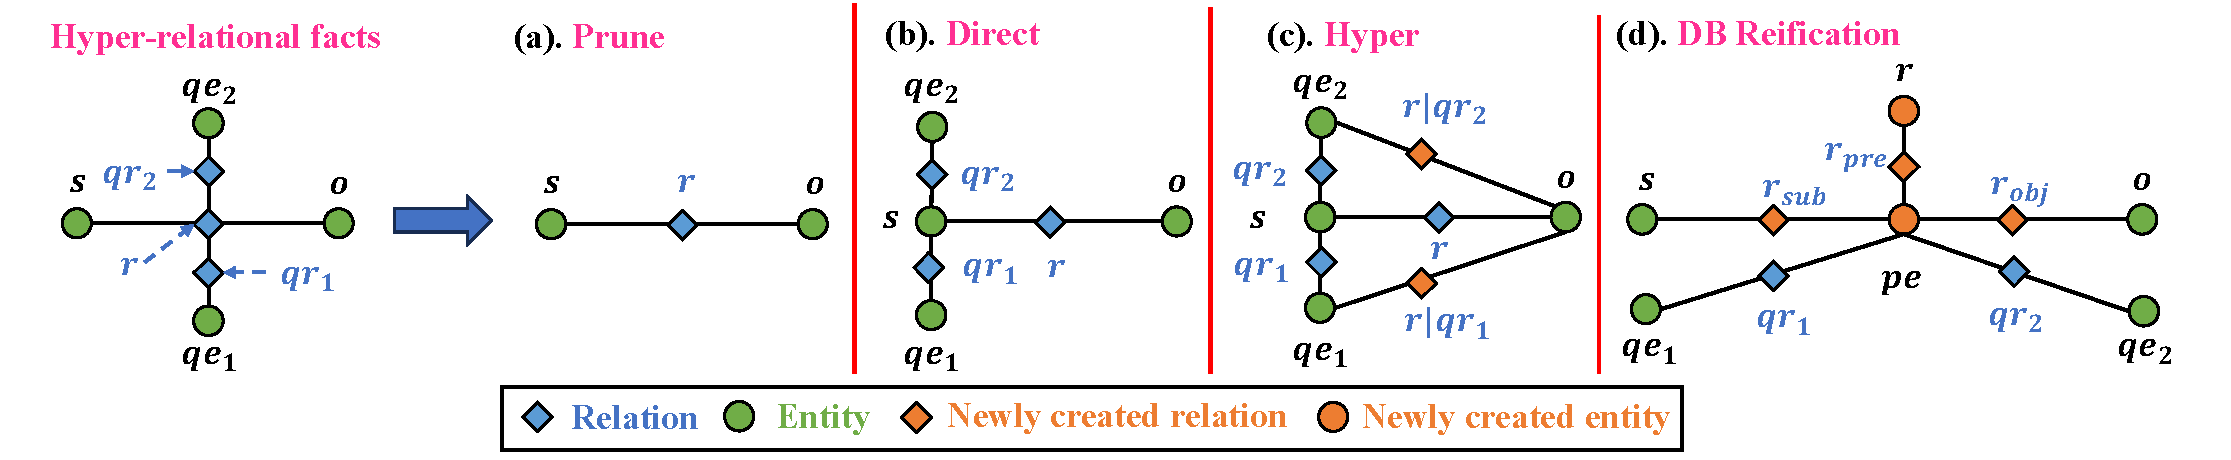
\includegraphics[width=\linewidth]{figures/hyperkg/decomp_new.pdf}
\caption{Original comparison of hyper-relational decomposition methods. Prune retains the main triple; Direct adds subject--qualifier links; Hyper adds combined relations; database reification introduces auxiliary objects. Reproduced from Fig.~1 of the CIKM study~\cite{bg-hyperkg}.}
\label{fig:background:decomposition}
\end{figure}

The association of a qualifier with a statement is especially relevant when a subject participates in several facts using the same relation. In the education example, a degree describes one university attendance statement. A collection of subject--degree and subject--university triples exposes the entities but changes the representation of which degree qualifies which attendance fact. A model following ordinary graph paths then receives the transformed connections. The Hyper method supplies additional connections intended to retain more of these associations, whereas a qualifier integrator receives the main fact and its qualifier pairs together. This comparison places information preservation at the interface between the data representation and the computation that follows it. It concerns the semantic organization of the input as well as its vocabulary.

The experiments compare conventional KGE models under these transformations with specialized HKGE models. Some GNN-based KGE configurations obtain scores comparable to specialized methods on Cleaned JF17k and WD50k. The observation motivates an examination of the represented information and the architecture receiving it. In particular, adding qualifier-derived edges can change the paths followed by a graph encoder. Preserving more items in a converted graph therefore changes the model's computational input as well as the nominal amount of stored information.

\subsection{Qualifier Capture and Graph Reception}

The analysis separates qualifier capture from graph reception. Qualifier capture concerns how the model represents qualifier pairs and their association with the main statement. Graph reception concerns how it receives information from the wider graph, including dependencies beyond one fact. Models operating on a fact in isolation have a different receptive field from graph encoders that propagate information across several hops. These properties are visible in the operations used to construct representations.

CompGCN jointly models entity and relation representations in a multi-relational graph~\cite{bg-compgcn}. NBFNet aggregates path information for link prediction~\cite{bg-nbfnet}. Their graph computations offer different ways to receive neighborhood and path information after decomposition. The CIKM analysis also identifies an information-compression issue when qualifier information is aggregated into fixed-size main-triple representations. Wider graph reception and qualifier integration consequently concern complementary parts of the architecture. The study evaluates designs that retain both sources for prediction.

FormerGNN combines a Transformer-based qualifier integrator operating on the original hyper-relational facts with a graph encoder operating on the pruned main-triple graph. The graph encoder generates a topology representation for the subject. The model concatenates this representation with representations of the main triple and qualifier pairs and passes them to a Transformer decoder. This organization supplies qualifier and graph information jointly to the prediction stage. In the reported configuration, HyperFormer provides the qualifier integrator and NBFNet provides the graph encoder~\cite{bg-hyperformer,bg-nbfnet}.

\subsection{Representative Published Evidence}

Table~\ref{tab:background:formergnn} reproduces the Cleaned JF17k and WD50k columns of the study's Table~6. It retains all seven model rows and all three metrics for those datasets. MRR measures mean reciprocal rank, and H@1 and H@10 measure whether the target entity appears within the corresponding rank cutoff. These are link-prediction measures, distinct from the annotation and answer metrics of the later chapters.

\begin{table}[tbp]
\centering
\caption{Projection of the CIKM study's Table~6 onto Cleaned JF17k and WD50k. All model rows and the original metric precision are retained; the original bold and underline markings indicate best and second-best values.}
\label{tab:background:formergnn}
\small
\begin{tabular}{lrrrrrr}
\toprule
&\multicolumn{3}{c}{Cleaned JF17k}&\multicolumn{3}{c}{WD50k}\\
\cmidrule(lr){2-4}\cmidrule(lr){5-7}
Model&MRR&H@1&H@10&MRR&H@1&H@10\\
\midrule
StarE&0.381&0.284&0.577&0.346&0.268&0.494\\
QUAD&0.402&0.305&0.602&0.349&0.275&0.487\\
HAHE&0.405&0.310&0.585&0.360&0.288&0.496\\
HyperFormer&\underline{0.425}&\underline{0.328}&0.613&\underline{0.372}&\underline{0.293}&0.522\\
NBFNet + Prune&0.415&0.313&\textbf{0.630}&0.360&0.271&\textbf{0.530}\\
CompGCN + Hyper&0.389&0.294&0.590&0.350&0.277&0.488\\
FormerGNN&\textbf{0.432}&\textbf{0.335}&\underline{0.624}&\textbf{0.377}&\textbf{0.299}&\underline{0.527}\\
\bottomrule
\end{tabular}
\end{table}

FormerGNN obtains MRR 0.432 on Cleaned JF17k and 0.377 on WD50k, compared with HyperFormer's 0.425 and 0.372. NBFNet + Prune has the highest H@10 in both selected datasets, at 0.630 and 0.530. The table therefore supports a metric-specific comparison. The experiment uses a single NVIDIA A100-40GB GPU. Parameters follow the original repositories or are selected by grid search when dataset-specific settings are unavailable. For comparisons involving CompGCN, the study replaces its decoder with a Transformer to align it with the corresponding HKGE configurations.

The complete published comparison also includes Wikipeople and FBAUTO, where dataset characteristics and metric rankings differ. The selected table illustrates graph reception and qualifier integration on these two datasets. The research establishes that the organization of graph information can matter beyond retaining the same entity and relation vocabulary. Its connection to this thesis is the design question of which relationships remain available to a model after evidence transformation. FormerGNN is a separate KG embedding framework; the four language-model systems use the structures and interfaces defined in their own chapters.

\section{Research Questions Emerging from the Background}
\label{sec:background:questions}

The preceding work identifies several places where structure can influence model inputs. Table understanding needs evidence that matches both the values and the task's type vocabulary. Dynamic classification needs an index that incorporates newly available label information and retrieves appropriate alternatives for the current text. Open-ended text generation needs a selection rule that can organize connected facts and retain their source context. Multimodal generation adds semantic matching across heterogeneous evidence and the cost of processing that evidence as model context.

The four research chapters address these conditions in sequence. Chapter~\ref{ch:kglink} studies external KG evidence and supervised type representations. Chapter~\ref{ch:gorag} studies connected candidate-label retrieval and online index updates. Chapter~\ref{ch:agrag} studies influence-aware connected evidence selection with hybrid passages. Chapter~\ref{ch:mgrag} studies query-aware multimodal graph construction, semantic path matching, and graph-aware KV recomputation. The hyper-relational study provides a related analysis of information preservation. The shared concern is how a representation exposes task-relevant evidence to the computation that uses it.

% Working chapter, 2026-10-24. Source checked against arXiv:2406.00318v1.
% The author confirmed that the linked arXiv PDF is publication-equivalent.
% Status AUTHOR_CONFIRMED_PUBLICATION_EQUIVALENT; not a direct publisher download.
% Author instruction: use publication prose to resolve internal prose/table conflicts.
% Detailed verification, source omissions, and remaining QA are in planning/verification-kglink.md.
\chapter{Knowledge-enriched Table Understanding with KGLink}
\label{ch:kglink}

This chapter is based on the published paper \emph{KGLink: A Column Type Annotation Method that Combines Knowledge Graph and Pre-Trained Language Model}~\cite{kglink-publication}. It studies how a knowledge graph can supply information missing from a table and how a pre-trained language model can translate that information into the type vocabulary of a particular annotation task. The prediction target is a column label. Graph evidence enters the model through candidate types and a separate feature sequence, while a supervised representation task connects the evidence to the dataset's annotation scheme.

\section{Motivation and Task}
\label{sec:kglink:motivation}

A table often presents entities through short names, abbreviated strings, or numbers. These values provide only part of the information needed to identify a column's semantic type. A column containing names of cricket players may appear beside birth and death dates. Those dates describe the people but do not specify their occupation. A language model that encodes only the table receives a different evidential basis from a model that also has access to relations such as occupation and sport in a knowledge graph. The annotation problem therefore concerns both interpreting the available text and selecting external information that clarifies it.

External knowledge introduces a second difficulty. The type expected by an annotation dataset need not coincide with a type attached to an entity in the graph. A column of basketball players can plausibly be described as \emph{Basketball player}, \emph{Athlete}, or \emph{Name}. An annotation benchmark may use only the last of these labels. Retrieving a factually relevant graph type is consequently insufficient to determine the required output label. The model must learn which description the task expects. KGLink refers to this mismatch as the type granularity gap. The gap includes cases where the desired dataset label does not occupy a convenient ancestor position in the retrieved graph's type hierarchy.

These two difficulties give structure distinct roles. Relations between linked entities can help identify relevant knowledge, while supervised learning can determine how that knowledge should influence a dataset-specific prediction. Treating graph types as final labels combines those roles too early. Treating the table as an isolated sequence omits the external relations. KGLink keeps graph evidence available to a learned classifier and trains an auxiliary task that generates a contextual representation of the target type. The learned classifier maps graph-derived evidence into the task's output classes.

The scope of the chapter is column-type annotation on the evaluated SemTab and modified VizNet datasets. Reasoning takes the form of inferring a semantic category from cells, their table context, and graph-derived evidence. The language model is an encoder trained for classification. Its output is drawn from the dataset's label set. This task establishes the first setting examined in the thesis, where an existing graph augments a model's representation before prediction.

\begin{figure}[tbp]
\centering
\begin{minipage}[b]{0.48\linewidth}
\centering
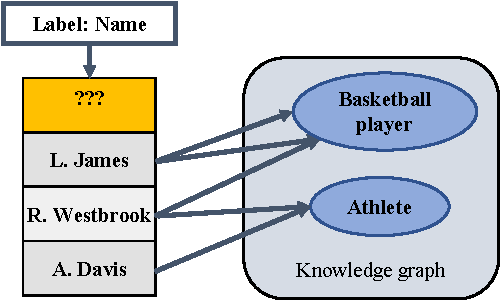
\includegraphics[width=\linewidth]{figures/kglink/tg_issue_small.pdf}
\par\small (a) Type granularity
\end{minipage}\hfill
\begin{minipage}[b]{0.48\linewidth}
\centering
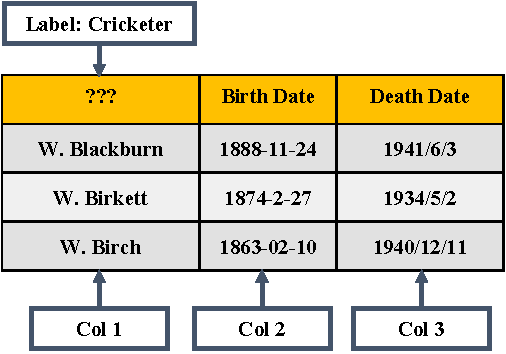
\includegraphics[width=\linewidth]{figures/kglink/DL_NotWell_small.pdf}
\par\small (b) Missing context
\end{minipage}
\caption{Two annotation difficulties in the original KGLink examples. A graph description such as Athlete can differ from the target label Name, while dates beside a person's name provide little occupation information. Original subfigures reproduced from KGLink~\cite{kglink-publication}, Fig.~2.}
\label{fig:kglink:motivation}
\end{figure}

\section{Problem Formulation and Framework}
\label{sec:kglink:problem}

Let $T$ be a table with row set $R$ and column set $C$. A cell mention $m_c^r$ is the content of row $r$ and column $c$. The task assigns a label $l_c$ from the dataset's type set $D$ to each target column. All columns in the same table can contribute context to that decision. The external knowledge graph supplies entity labels and their one-hop relations. During training, column labels supervise both classification and the auxiliary representation task. During evaluation, those labels are absent from the model input.

KGLink has a graph-processing stage followed by a language-model stage. The graph stage retrieves candidate entities for cell mentions, filters these entities using connections between columns, ranks rows by their linkage quality, and derives candidate types from the remaining entities' neighborhoods. It also constructs a feature sequence for each target column. The language-model stage serializes the processed table, encodes the table and feature sequences, combines the resulting representations, and predicts the column labels. A second training input contains the true type labels and provides contextual supervision for representations generated from masked type positions.

Figure~\ref{fig:kglink:framework} shows the two stages and their training objectives.

\begin{figure}[tbp]
\centering
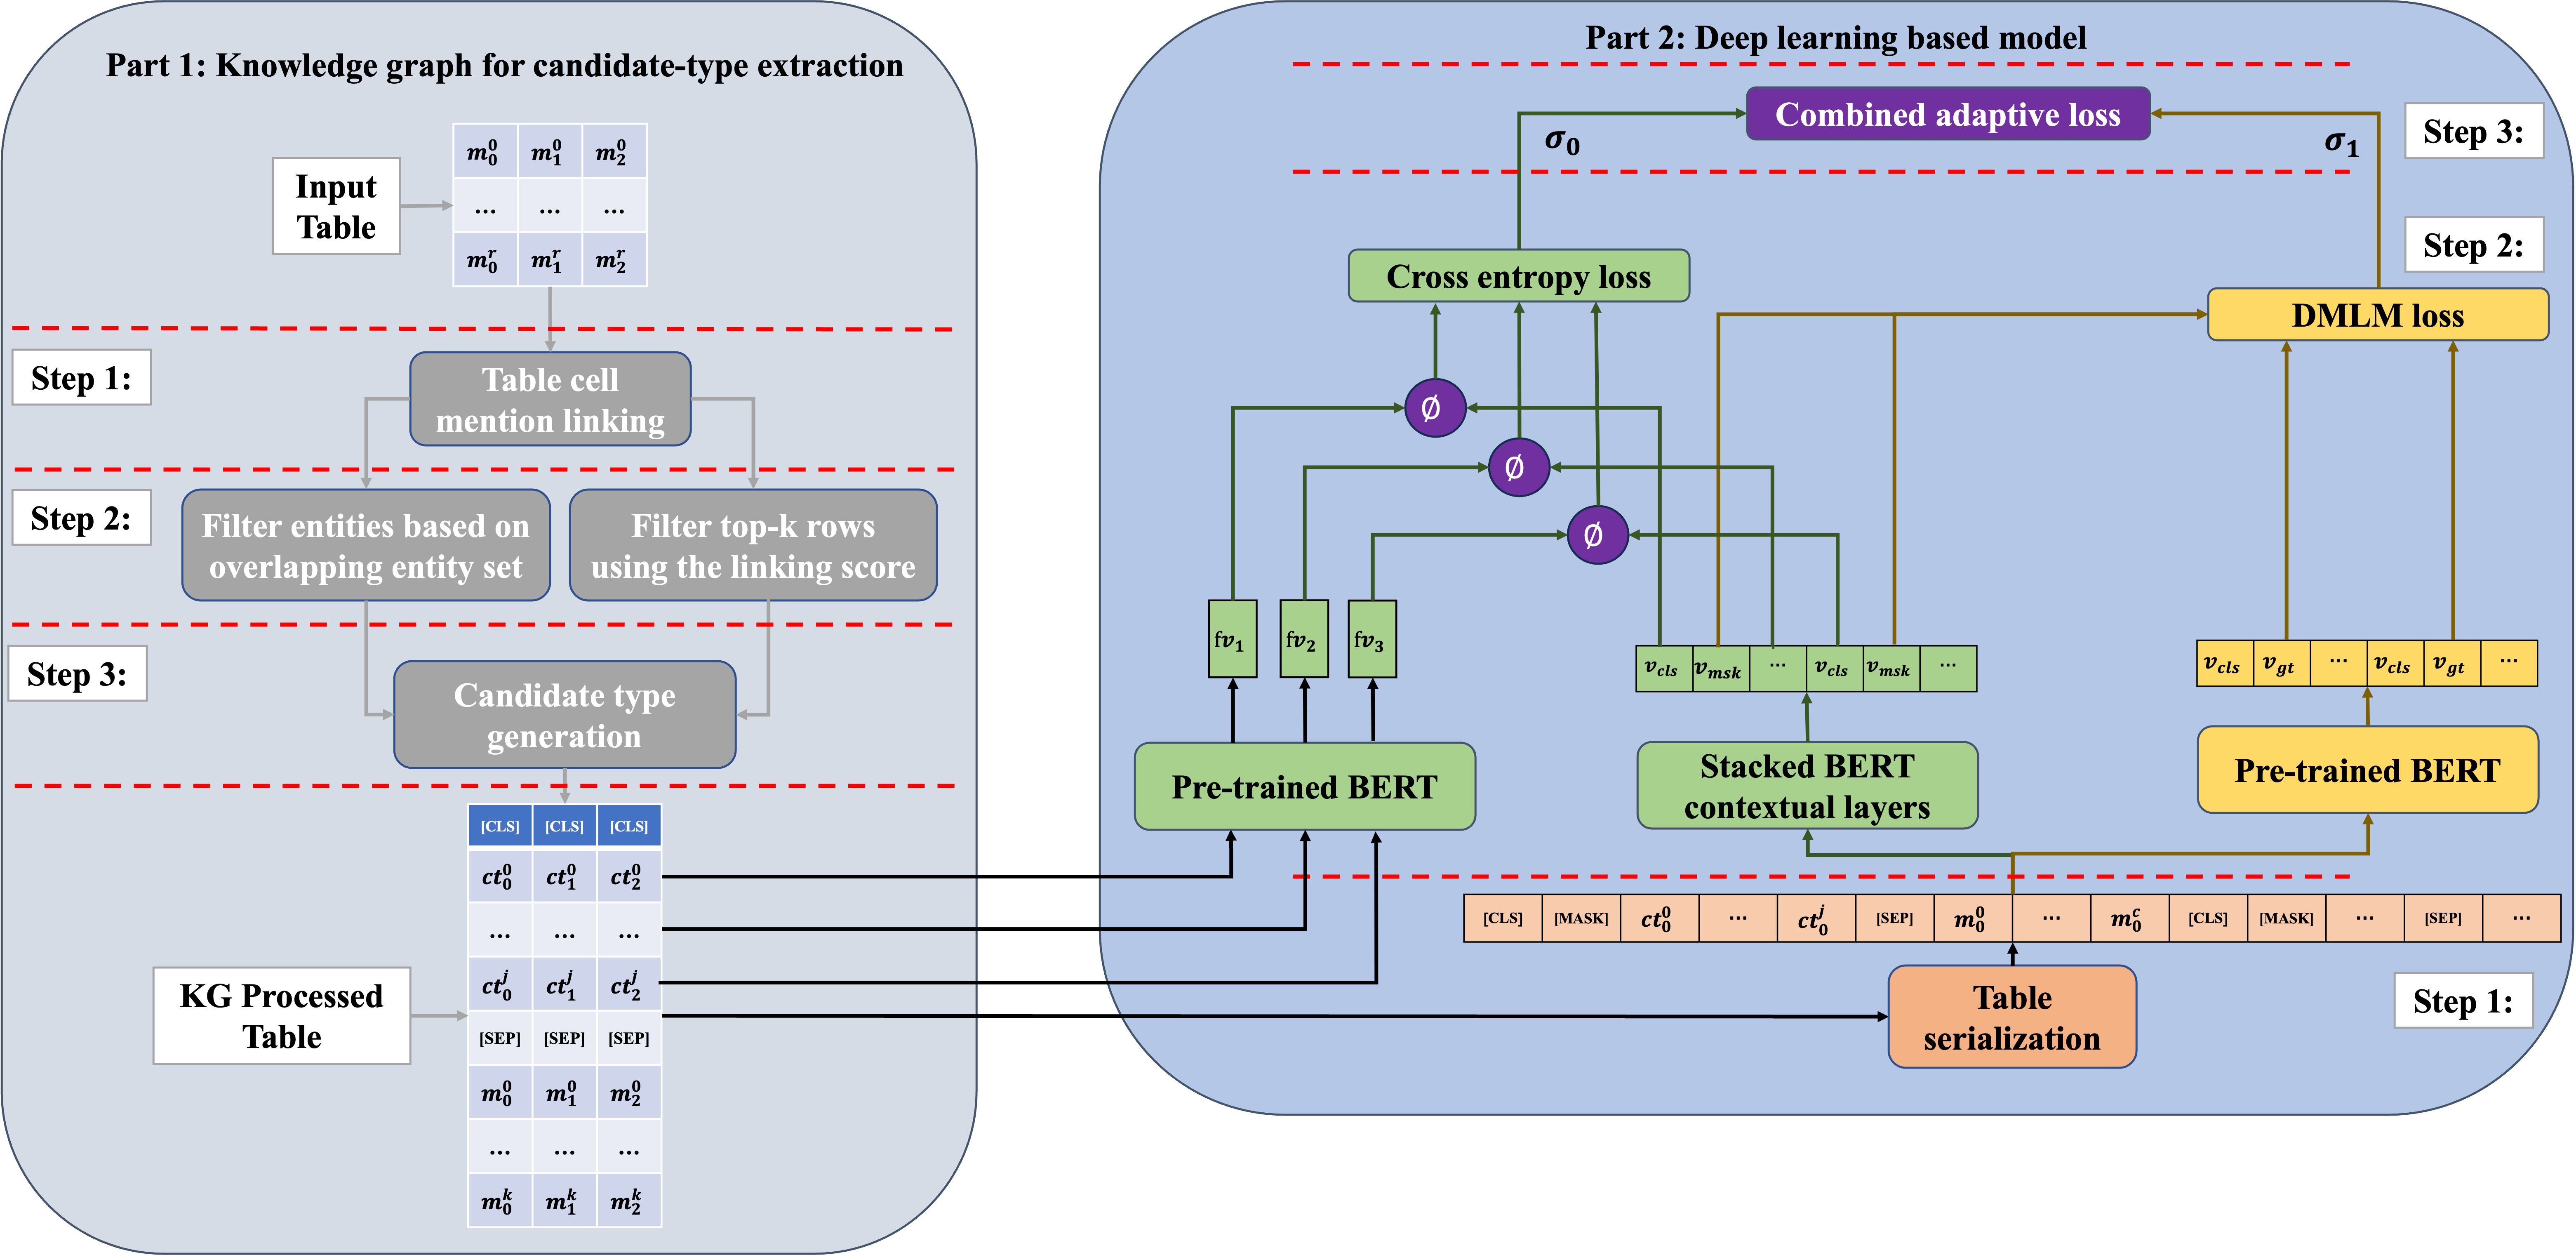
\includegraphics[width=\linewidth]{figures/kglink/kglink_new_overview.png}
\caption{KGLink's graph-processing and language-model components. Candidate-type text, column feature vectors, and a contextual type-representation objective connect external knowledge to annotation. Original image reproduced from KGLink~\cite{kglink-publication}, Fig.~3.}
\label{fig:kglink:framework}
\end{figure}

The two graph inputs have different selection rules. Candidate types aggregate evidence across linked cells and retain types supported by the column. A feature sequence describes a selected linked entity and its neighboring relations. The latter supplies another route for KG information when candidate-type selection produces little evidence. Neither input changes the classifier's output vocabulary. For example, a candidate type describing an occupation can support a broader annotation category through the learned model even when the strings differ.

The framework also controls the amount of table content passed to the encoder. Entity linking and row selection precede serialization. The retained rows provide a bounded view of the table, and wide tables are split by columns under the reported input constraints. These operations matter because inserting external knowledge competes with cell content for the encoder's finite input length. KGLink selects graph evidence and table rows before encoding.

\section{KG-derived Candidate Types}
\label{sec:kglink:candidates}

\subsection{Cell Mention Linking}
\label{sec:kglink:linking}

The first step retrieves a candidate entity set $E_{m_c^r}$ for each suitable cell mention. KGLink uses BM25 to score the relation between the mention's words and indexed entity labels~\cite{kglink-robertson2009probabilistic}. The implementation indexes Wikidata with Elasticsearch. The score incorporates query-term frequency, inverse document frequency, and label-length normalization. Multiple entities can match the same mention, so the retrieval output is a candidate set rather than a single disambiguated entity.

This distinction is relevant for short strings. An album title and an ordinary word may share the same surface form, while a person's name can refer to several people. Lexical matching can identify plausible entries without determining which one belongs in the current table. KGLink uses the table's row structure in the next step to provide this disambiguating context. A cell's candidate set is consequently an intermediate object whose members can be removed when their graph relations disagree with evidence from other columns.

Numeric and date mentions are handled separately. The reported procedure uses named-entity detection to identify these mentions and assigns them a linking score of zero. A failed entity lookup also receives a zero linking score. The subsequent model still receives the table values, so absence of a graph link does not remove a column from the annotation task. The language-model component provides the classification pathway for columns with missing KG evidence.

The experimental implementation retrieves at most ten entities per cell mention. This limit bounds the candidate sets that enter the subsequent neighborhood operations. Graph-based filtering and row ranking select among the retrieved evidence before it reaches the annotation model.

\subsection{Cross-column Neighborhood Filtering}
\label{sec:kglink:filtering}

\begin{figure}[tbp]
\centering
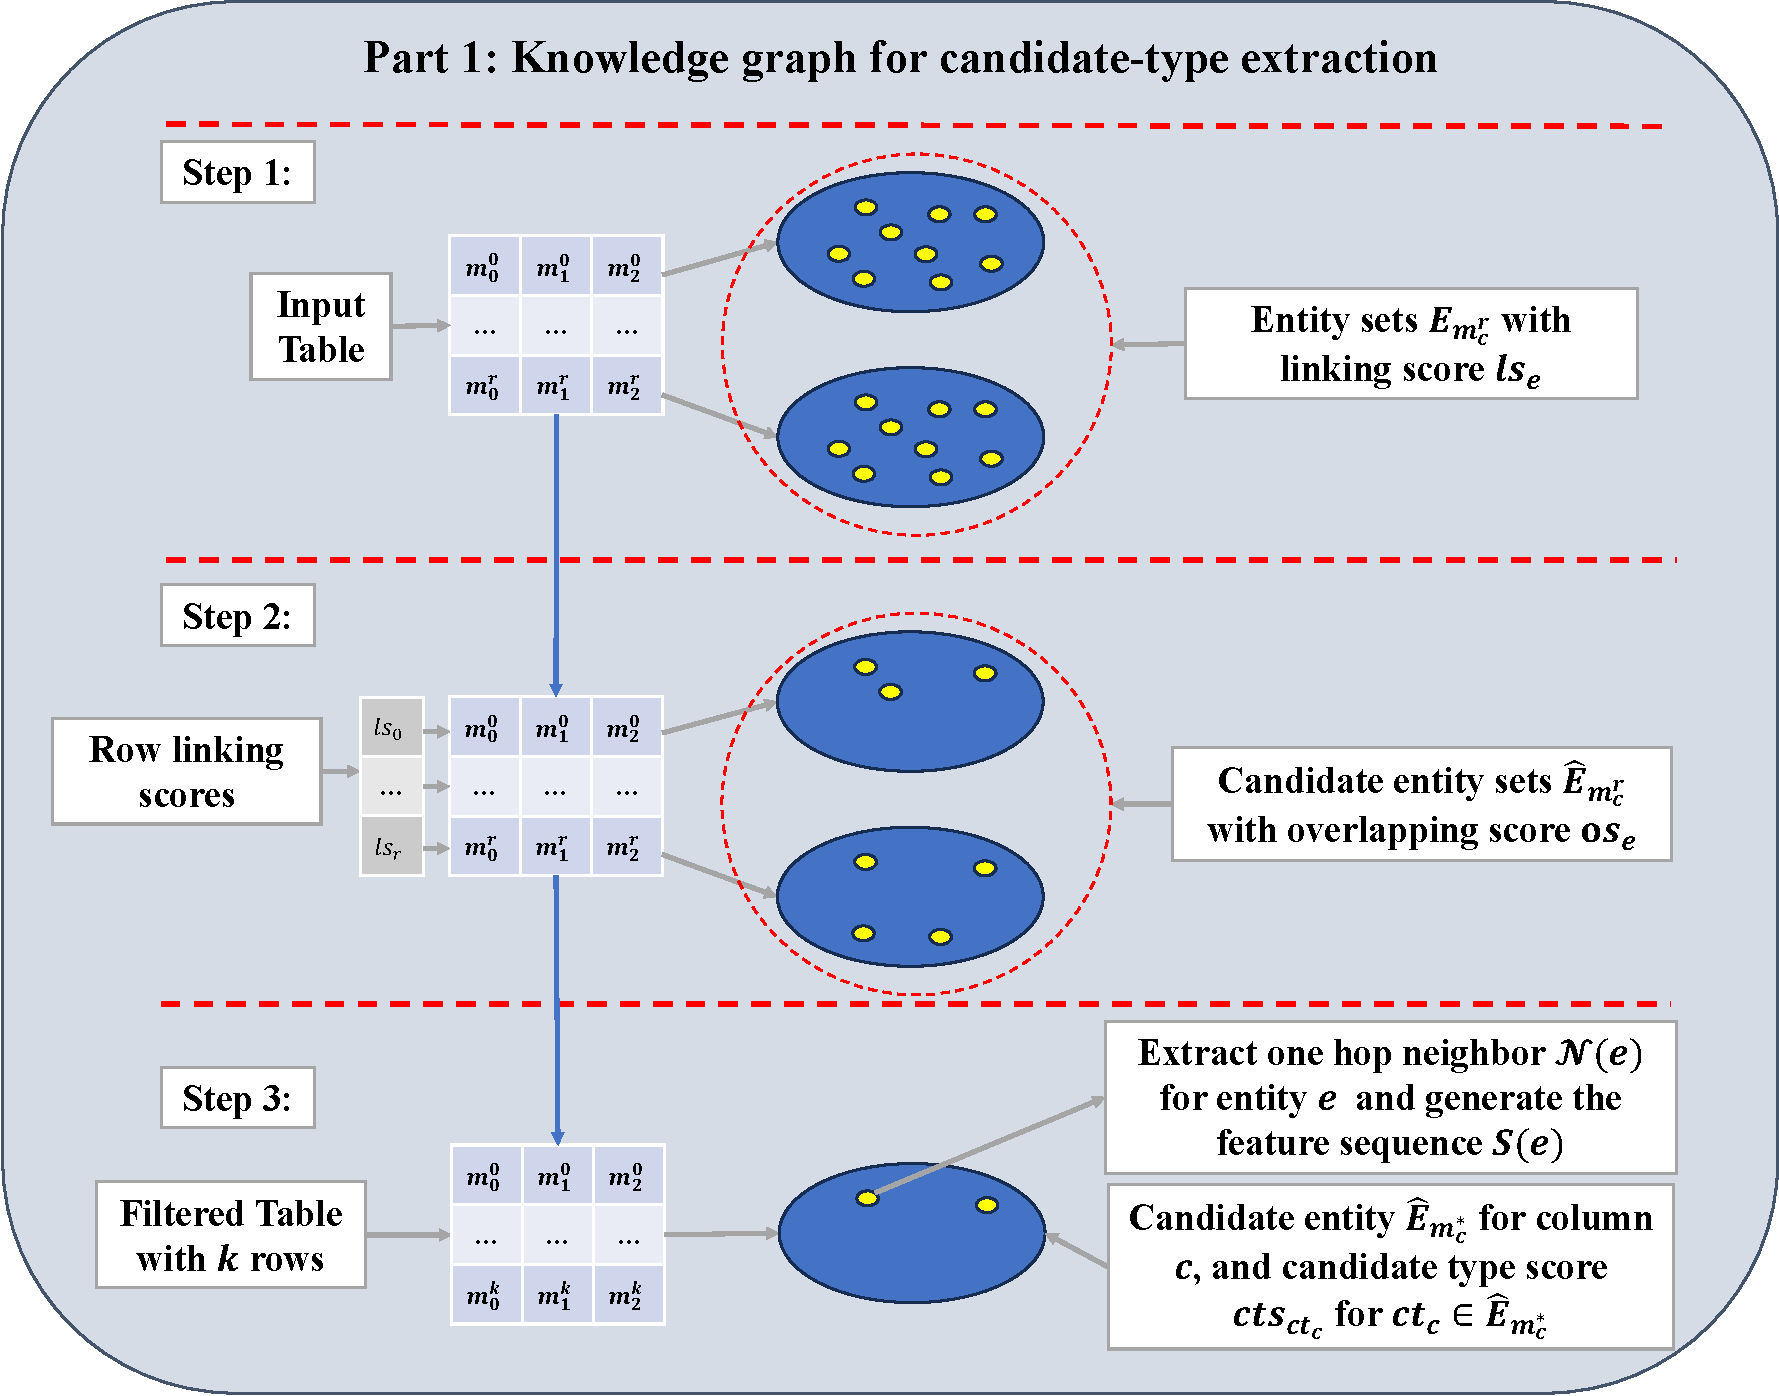
\includegraphics[width=0.76\linewidth]{figures/kglink/KG_part.pdf}
\caption{The original KG-processing pipeline. Cell linking is followed by entity filtering, row selection, and candidate-type generation. Reproduced from KGLink~\cite{kglink-publication}, Fig.~4.}
\label{fig:kglink:kg-pipeline}
\end{figure}

Cells in the same row describe related objects. An album title beside a musician's name supplies a useful relation that either mention lacks in isolation. KGLink uses this relation by checking whether a candidate entity for one cell occurs in the one-hop neighborhood of candidates for another cell in the same row. Let $\mathcal{N}(E)$ denote the one-hop neighbors of a candidate entity set. The filtered set for a cell is
\begin{equation}
\widehat{E}_{m_{c_1}^{r}}
 = \bigcup_{c_2\in C\setminus\{c_1\}}
 \left(E_{m_{c_1}^{r}}\cap\mathcal{N}(E_{m_{c_2}^{r}})\right).
\label{eq:kglink:entity-filter}
\end{equation}
The union allows support from any other column. The intersection retains entities retrieved for the target mention that also have the required neighborhood support.

Figure~\ref{fig:kglink:overlap} uses \emph{Rust} and \emph{Peter Steele}. A graph connection between an album candidate and the musician candidate supports their interpretation as the entities intended by the row. The role of the edge is to constrain which external facts are relevant to the table. KGLink subsequently associates each retained entity with an overlapping score that counts its neighborhood support from other columns. Entities with more such support contribute more to candidate-type selection.

Neighborhood support is a structural selection signal. It depends on the relations recorded in the external graph and on the initial entity candidates. A missing graph relation can remove useful evidence, while an incorrect lexical candidate can survive if it has matching contextual links. The model therefore also uses the original table sequence and a separate feature representation. This architecture gives graph filtering a specific responsibility, selecting evidence for the classifier, without making its output the classifier's final decision.

\begin{figure}[tbp]
\centering
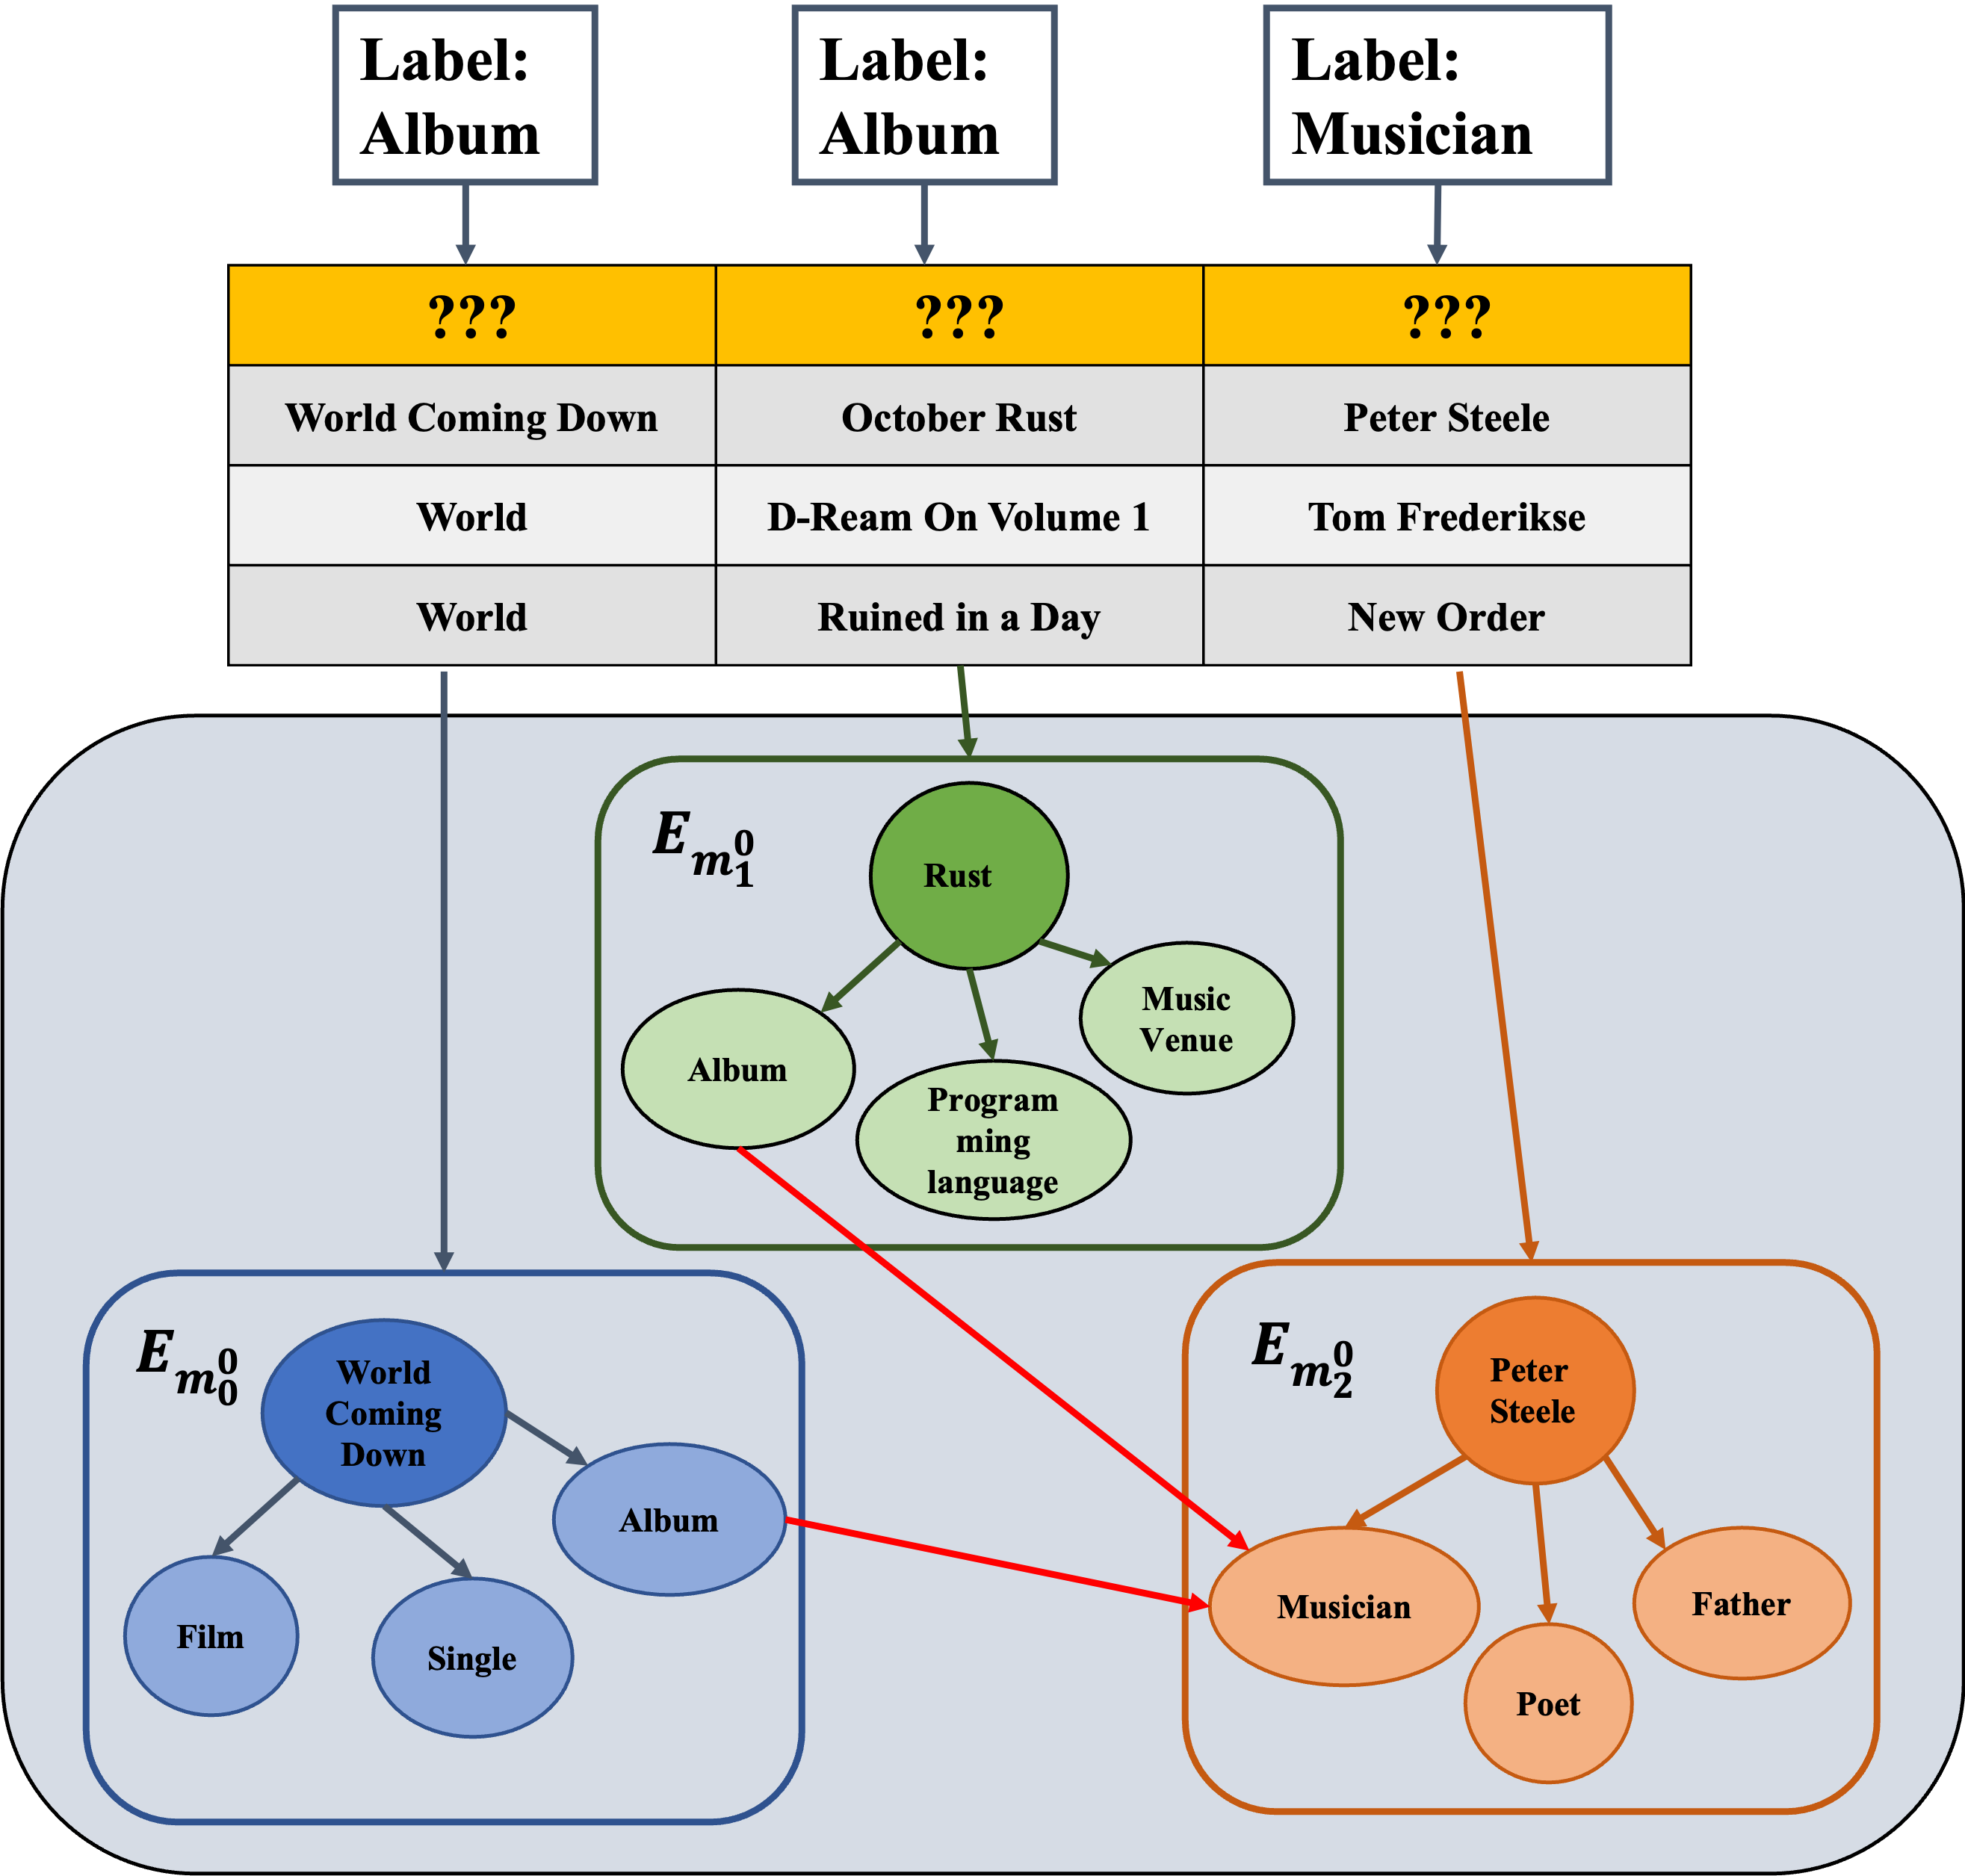
\includegraphics[width=0.75\linewidth]{figures/kglink/overlap.png}
\caption{Cross-column evidence in the original album-and-musician example. Graph links connect candidate interpretations of cell mentions in the same row. Original image reproduced from KGLink~\cite{kglink-publication}, Fig.~5.}
\label{fig:kglink:overlap}
\end{figure}

The filter uses inter-column information within a row, whereas candidate-type generation aggregates across rows within a column. These are different structural assumptions. The first exploits the relation between attributes of the same record. The second looks for recurring semantic descriptions of several values occupying the same column. Separating them clarifies why a relevant neighbor of one entity is insufficient on its own to determine a column's type.

\subsection{Row Linking Quality and Input Selection}
\label{sec:kglink:rows}

KGLink derives a cell score from the best-scoring retained entity. For a nonempty filtered candidate set, the score is
\begin{equation}
ls_{m_c^r}=\max_{e\in\widehat{E}_{m_c^r}}ls_e,
\label{eq:kglink:cell-score}
\end{equation}
where $ls_e$ is the entity's BM25 linking score. Unlinked cells use zero as described in the evaluation protocol. A row's score sums the scores of its cells,
\begin{equation}
ls_r=\sum_{c\in C}ls_{m_c^r}.
\label{eq:kglink:row-score}
\end{equation}
Rows are sorted by this quantity, and only the top $k$ rows are retained for prediction.

This operation changes which examples of a column the language model observes. Selecting the first $k$ rows preserves the source table's order; ranking by linkage favors rows with more lexically supported graph evidence after filtering. The latter can make the external evidence more useful within the same row budget. The row-filter experiment compares the two selection rules while retaining the reported input limit.

Row selection also connects the graph and feature pathways. The feature sequence is generated from a selected cell associated with the highest-ranked row. Changing the row order can therefore affect the table content and the KG entity used to form that sequence. The row-selection experiment evaluates this coupled selection mechanism.

\subsection{Candidate Types and Feature Sequences}
\label{sec:kglink:types-features}

Candidate-type generation searches beyond an entity's explicit type attribute. A person's graph entry may be typed as \emph{Human}, while \emph{Musician} appears as an occupation neighbor. The latter can be more informative for a table column. KGLink collects filtered entities across the target column and examines their one-hop neighborhoods. It scores a potential type by aggregating the overlapping scores of entities from other rows that connect to that type. Repeated support within the column increases the candidate's score.

A label-based filter excludes candidates assigned the named-entity schema categories \texttt{PERSON} or \texttt{DATE}. The reported implementation uses spaCy for this step. This filter distinguishes a descriptive candidate type from a particular person's name or a date encountered in the neighborhood. KGLink retains the selected candidate-type labels as text and places them before the cell values in the processed column. The reported implementation generates up to three candidate types per row from the KG entities in each column. Their later contribution depends on how the encoder interprets them in the table context.

If no candidate type is returned, padding occupies the corresponding position. Numeric columns use numeric summary information in this part of the input, while their original values remain available in the table sequence.
% Source issue: “mean, variance, and average value” duplicates mean/average.
% Keep the exact list out of final method specification until author/publisher resolution.

The feature sequence provides a second representation of the retrieved knowledge. From the filtered and ranked table, KGLink selects a cell for each target column, chooses its highest-linking entity, and serializes that entity with its one-hop predicates and neighboring entities. If $e$ is the selected entity, $p$ a predicate, and $o$ a neighboring object, the sequence consists of the entity label followed by predicate--object descriptions. Encoding this text yields a feature vector for the column. A padding sequence is used when the column has no retrieved entity.

Candidate types and feature sequences thus preserve different aspects of a neighborhood. Candidate selection emphasizes descriptions recurring across column values. The feature sequence retains relational details surrounding a particular well-linked value. The experimental ablations examine the two pathways through specific model variants.

\section{Language Model Integration}
\label{sec:kglink:language-model}

\subsection{Table Serialization and Column Representations}
\label{sec:kglink:serialization}

KGLink adapts the multi-column serialization used by Doduo~\cite{kglink-suhara2022annotating}. A special \texttt{[CLS]} token begins each column's segment. The segments are concatenated into one input sequence, followed by a \texttt{[SEP]} token. The contextual representation at each column's \texttt{[CLS]} position provides that column's vector. Because the sequence contains multiple columns, self-attention can use information outside the predicted column.

Writing the tokenized contents of column $i$ as $\mathrm{tok}_i^1,\ldots,\mathrm{tok}_i^{m}$, the original multi-column serialization has the form
\begin{equation}
\begin{split}
S(T)={}&[\mathrm{CLS}]\ \mathrm{tok}_1^1\cdots\mathrm{tok}_1^m\ 
[\mathrm{CLS}]\ \mathrm{tok}_2^1\cdots\\
&[\mathrm{CLS}]\ \mathrm{tok}_{|C|}^1\cdots\mathrm{tok}_{|C|}^m\ 
[\mathrm{SEP}].
\end{split}
\label{eq:kglink:serialization}
\end{equation}
Each column's \texttt{[CLS]} position produces a contextual vector using the serialized columns. Candidate-type text precedes the corresponding cell values, allowing both to interact with neighboring columns through self-attention. KGLink separately encodes the feature sequence into a column-specific vector and combines it with the contextual column vector through the composition function $\phi$. The resulting representation is mapped into the dataset's classification space.

The principal experiments fine-tune BERT~\cite{kglink-devlin2018bert}. The model has a sequence limit of 512 tokens; the reported implementation limits each column to 64 tokens and each encoded table to eight columns. Tables with more columns are divided after candidate-type generation and are encoded separately. These limits define the context available to the classifier. In particular, retaining 25 table rows does not imply that every token in those rows survives serialization, since tokenization and the column limit also constrain the final sequence.

\subsection{Contextual Type Representation Learning}
\label{sec:kglink:representation}

The auxiliary task trains a type representation at a masked position. During training, KGLink constructs two versions of the processed table. The ground-truth version places the annotated type label before the candidate types in each target column. The masked version replaces that label with \texttt{[MASK]}. Both versions retain the column values and candidate-type context. Encoding the two sequences produces contextual representations for the true type and its masked counterpart.

Figure~\ref{fig:kglink:representation} illustrates the two inputs and their contextual outputs.

\begin{figure}[tbp]
\centering
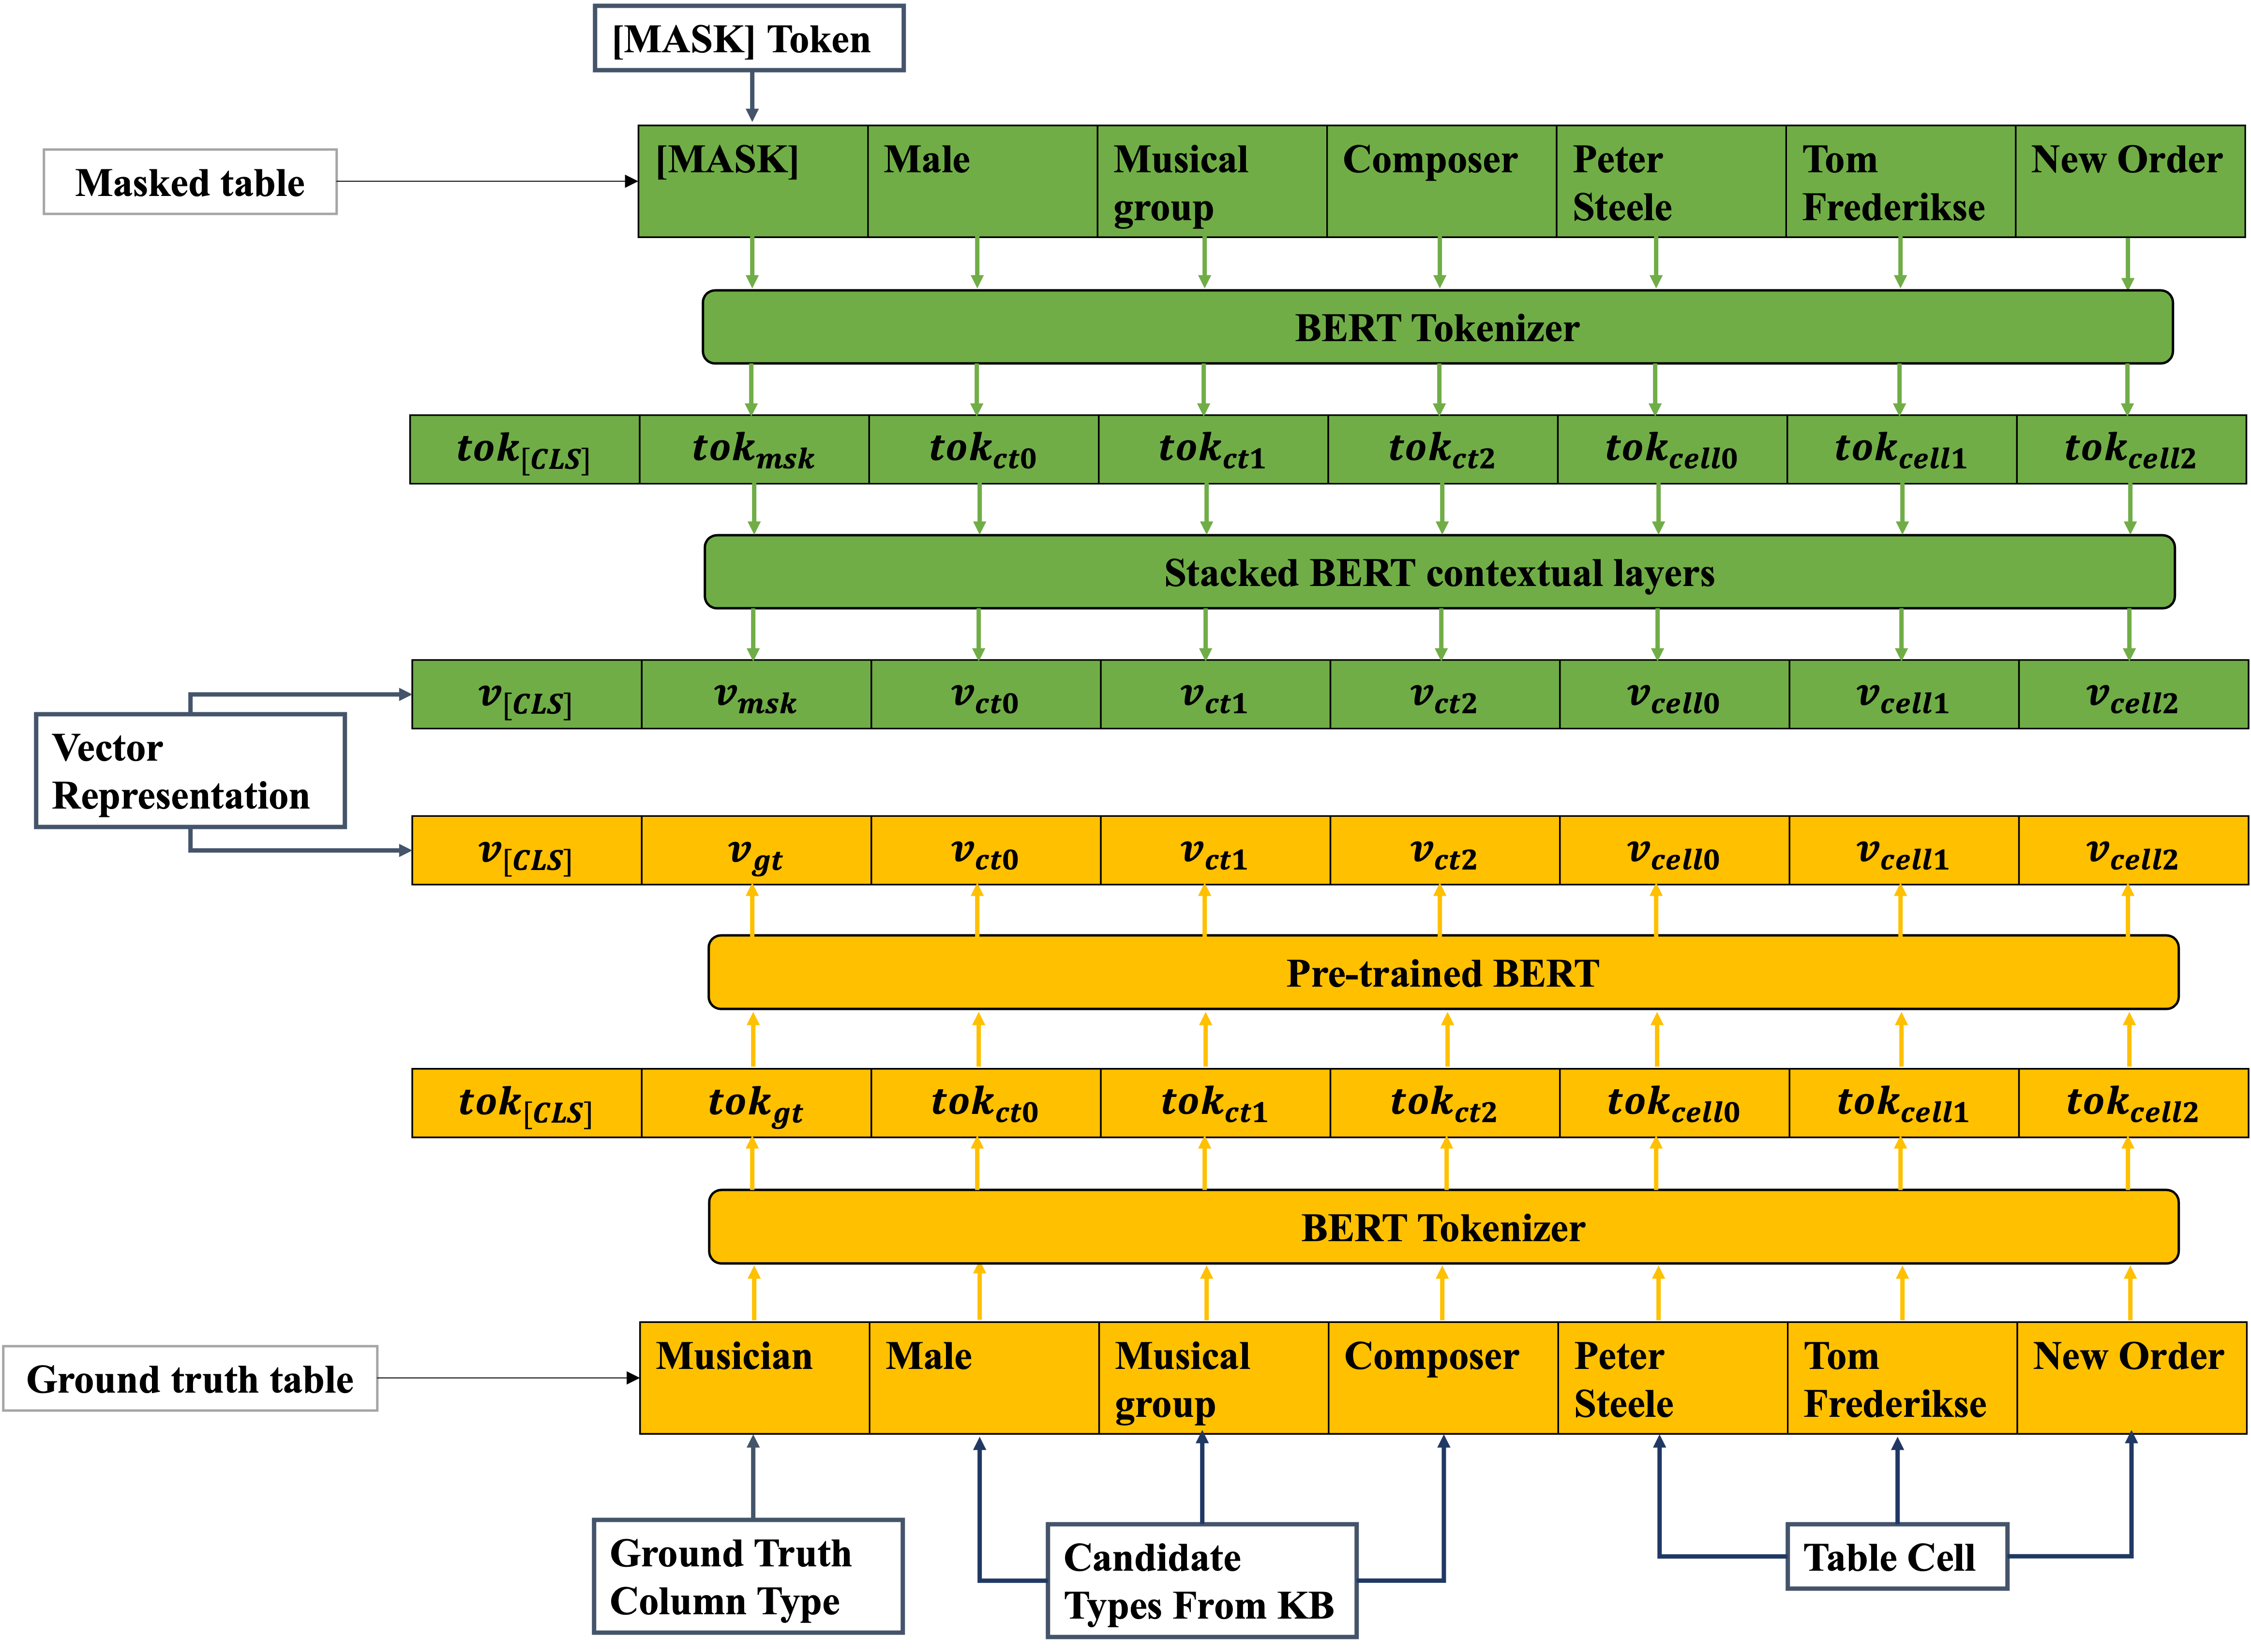
\includegraphics[width=\linewidth]{figures/kglink/dmlm.png}
\caption{Contextual type-representation training with masked and ground-truth table inputs. The true-type table is constructed during training. Original image reproduced from KGLink~\cite{kglink-publication}, Fig.~6.}
\label{fig:kglink:representation}
\end{figure}

This arrangement supplies supervision about the label's meaning in context. A label such as \emph{Musician} is encoded together with the column values and graph-derived descriptions, rather than as an isolated word. The masked input must produce its type representation from the evidence that will be available at prediction time. Distilled masked language modeling provides the auxiliary objective~\cite{kglink-wang2020learning}. The model projects contextual representations into vocabulary space with a temperature parameter, then uses the ground-truth and masked outputs in the reported training loss.

With contextual vector $H$ and temperature $\mathcal{T}$, vocabulary projection gives
\begin{equation}
Y=\operatorname{Softmax}\!\left(W_o\frac{H}{\mathcal{T}}\right),
\label{eq:kglink:vocabulary-projection}
\end{equation}
where $W_o$ projects into the vocabulary space. Denote the masked and ground-truth outputs by $Y_{\mathrm{msk}}$ and $Y_{\mathrm{gt}}$. The main paper writes the auxiliary objective as
\begin{equation}
\mathcal{L}_{\mathrm{DMLM}}(Y_{\mathrm{msk}},Y_{\mathrm{gt}})
=-\sum_{j=1}^{V}y_{\mathrm{msk}}^{j}\log y_{\mathrm{gt}}^{j},
\label{eq:kglink:dmlm}
\end{equation}
with vocabulary size $V$. The objective uses the contextualized representations produced from the two table inputs.

Training uses the true-type and masked inputs, while evaluation uses the masked input. The auxiliary objective therefore learns from labels available in training and generates a type representation from the ordinary table and retrieved evidence at prediction time. This pathway also serves numeric columns and columns without a retrieved KG candidate.

The classifier and the auxiliary task also use different output spaces. Classification predicts one of the dataset's column labels. The auxiliary representation is projected into the language model's vocabulary space. Their relationship is learned through the shared encoder and joint training. The final decision uses the dataset-specific classification head.
% Author directed main-text precedence; Eq. dmlm preserves source order exactly.

\subsection{Classification and Adaptive Task Weighting}
\label{sec:kglink:objective}

Let $z_c$ be the classification logits obtained from the combined column and feature representations. For a target label $l_c$, the classification loss is cross-entropy,
\begin{equation}
\mathcal{L}_{\mathrm{CE}}(z_c,l_c)
 =-\log\frac{\exp(z_{c,l_c})}{\sum_{j\in D}\exp(z_{c,j})}.
\label{eq:kglink:classification}
\end{equation}
KGLink jointly optimizes this loss and the auxiliary representation objective using uncertainty weighting~\cite{kglink-kendall2018multi}. With trainable task parameters $\sigma_0$ and $\sigma_1$, the combined objective is
\begin{equation}
\mathcal{L}_{\mathrm{total}}
 =\frac{\mathcal{L}_{\mathrm{DMLM}}}{2\sigma_0^2}
  +\frac{\mathcal{L}_{\mathrm{CE}}}{2\sigma_1^2}
  +\log(\sigma_0\sigma_1).
\label{eq:kglink:joint-loss}
\end{equation}
The temperature used in the representation objective is set to two in the reported experiments.

The trainable weights allow the two objectives to contribute at different scales during optimization. They weight the training objectives, while row linking scores govern input selection. These mechanisms connect graph evidence to prediction at different stages of the pipeline.

\section{Computational Structure}
\label{sec:kglink:complexity}

The graph-processing cost depends on table dimensions, candidate-set sizes, and neighborhood sizes. Linking traverses table cells. Cross-column filtering compares candidate information between columns within a row. Candidate-type scoring visits neighborhoods and aggregates support across rows. The implementation's limits on retrieved entities and serialized columns constrain these operations in the evaluated setting. The external Wikidata index is prepared with Elasticsearch and supplies lexical retrieval scores.

The original analysis denotes maximum table rows and columns by $R$ and $C$, the number of tables by $T$, the maximum retrieved entities by $E$, and their maximum one-hop neighborhood size by $N$. It reports the preprocessing expression
\begin{equation}
O\!\left(RCE(N+CET)\right).
\label{eq:kglink:preprocessing}
\end{equation}
The expression includes neighborhood aggregation and the cross-column candidate operations. It makes explicit that table dimensions and graph retrieval size affect preprocessing even when the later encoder length is capped. An increased candidate-set limit changes the graph-processing workload before any table tokens are encoded.

Encoding cost depends on the serialized input length and the encoder's hidden dimension. KGLink encodes table inputs and column feature sequences; training also includes the ground-truth and masked constructions used by the representation task. The classification head maps column vectors into the label space, while the auxiliary projection operates over the language model's vocabulary. Thus, increasing the label set affects classification, whereas increasing the vocabulary-space projection concerns the representation objective.

These costs describe different resources. Reducing the retained row count can shorten preprocessing or input preparation without proportionally changing a sequence already truncated to its token limit. Increasing candidate retrieval can add neighborhood work even when the encoder input remains fixed. The runtime and row-budget studies should therefore be read alongside the input protocol. The measurements use the reported input bounds and hardware.

\section{Experimental Evaluation}
\label{sec:kglink:experiments}

\subsection{Datasets and Protocol}
\label{sec:kglink:protocol}

The evaluation uses SemTab 2019 and a modified VizNet subset~\cite{kglink-hassanzadeh_oktie_2019_3518539,kglink-zhang2020sato}. SemTab includes tables derived from Wikipedia, DBpedia, and the T2Dv2 Gold Standard sources. The experiment uses rounds 1, 3, and 4, with 3,048 tables, 7,587 columns, and 275 column types. Round 2 has columns with multiple ground-truth labels and is excluded from this single-label comparison. The reported averages are 69 rows and 4.5 columns per table.

The modified VizNet corpus targets column annotation rather than the full range of visualization tasks in the original repository~\cite{kglink-hu2019viznet}. The experiment uses its multi-column portion so that methods can exploit relations between columns. Its annotation scheme is coarser than SemTab's and includes numeric types. The evaluated portion contains 32,265 tables, 73,034 annotated columns, and 77 types.
% Dataset prose: 73,034 columns; source Table III: 74,141 columns.
% Do not select a denominator or recompute the original percentages.

The data are split into training, validation, and testing portions in the ratio 7:1:2 while maintaining each class's original sample proportion. The original study averages each experiment over three runs. It reports accuracy and weighted F1; these assess exact prediction of the target annotation label and class-frequency-weighted classification performance. A graph candidate that is semantically related to the answer still needs to produce the dataset label to count as a correct classification.

Training uses AdamW, an initial learning rate of $3\times10^{-5}$, and $\epsilon=10^{-6}$. The learning rate decays linearly without warm-up. The reported maximum training lengths are 50 epochs on SemTab and 20 on VizNet, with early stopping. Batch size is 16 for both datasets; dropout is 0.1 for SemTab and 0.2 for VizNet. The implementation uses PyTorch and the Transformers library on an NVIDIA Tesla V100 GPU.

The baseline set includes MTab, TaBERT, Doduo, HNN, Sudowoodo, and RECA~\cite{kglink-2021_mtab4wikidata,kglink-yin2020tabert,kglink-suhara2022annotating,kglink-chen2019learning,kglink-wang2022sudowoodo,kglink-sun2023reca}. TaBERT and Doduo use KGLink's experimental settings. HNN and RECA follow their original settings. Sudowoodo receives the full labeled training set in this comparison. VizNet labels are translated to Wikidata entities for MTab, and MTab's weighted F1 is unreported because of the difference in problem definition. 

\subsection{Main Annotation Results}
\label{sec:kglink:main-results}

\begin{table}[tbp]
\centering
\caption{Column-type annotation results reported for KGLink. Scores and missing entries reproduce the original main-result table.}
\label{tab:kglink:main}
\begin{tabular}{lrrrr}
\toprule
&\multicolumn{2}{c}{SemTab}&\multicolumn{2}{c}{VizNet}\\
\cmidrule(lr){2-3}\cmidrule(lr){4-5}
Model&Accuracy&Weighted F1&Accuracy&Weighted F1\\
\midrule
MTab&\textbf{89.10}&-&38.21&-\\
TaBERT&72.69&71.21&94.68&94.07\\
Doduo&84.06&82.43&95.40&95.06\\
HNN&66.54&65.12&66.89&68.82\\
Sudowoodo&79.34&79.24&91.57&91.08\\
RECA&86.12&84.91&93.25&93.18\\
KGLink&87.12&\textbf{85.78}&\textbf{96.28}&\textbf{96.07}\\
\bottomrule
\end{tabular}
\end{table}

Table~\ref{tab:kglink:main} reports the main comparison. KGLink obtains accuracy 87.12 and weighted F1 85.78 on SemTab, and accuracy 96.28 and weighted F1 96.07 on VizNet. MTab has the highest SemTab accuracy, 89.10. KGLink has the highest reported weighted F1 on SemTab and the highest values of both reported metrics on VizNet. These distinctions matter because the baseline comparison contains a task-definition difference for MTab and does not include its weighted F1.

Doduo provides a useful comparison for the language-model pathway because KGLink adapts its serialization and uses BERT in the main configuration. Doduo obtains 84.06 accuracy on SemTab and 95.40 on VizNet. KGLink's higher scores under the reported experiment indicate that the full graph-augmented and jointly trained model improves on that baseline. The component experiments below examine which parts of KGLink contribute; the main table alone compares complete methods.

The dataset dependence is also visible in MTab's results. Its accuracy is 89.10 on SemTab and 38.21 on VizNet under the label translation used in the experiment. These measurements motivate separating graph knowledge from the final annotation vocabulary. The source evaluates supervised methods and a KG-based method whose label assumptions differ. The resulting scores describe performance under each dataset's label vocabulary and protocol.

\subsection{Representation Learning and KG Evidence}
\label{sec:kglink:ablation}

\begin{table}[tbp]
\centering
\caption{Reported KGLink variant scores. The table reproduces the numeric columns and variant names of the original ablation table.}
\label{tab:kglink:ablation}
\begin{tabular}{lrrrr}
\toprule
&\multicolumn{2}{c}{SemTab}&\multicolumn{2}{c}{VizNet}\\
\cmidrule(lr){2-3}\cmidrule(lr){4-5}
Variant&Accuracy&Weighted F1&Accuracy&Weighted F1\\
\midrule
KGLink $w/o\ msk$&86.14&84.54&95.95&95.67\\
KGLink $w/o\ ct$&86.27&84.56&95.83&95.48\\
KGLink $w/o\ fv$&87.02&85.68&95.98&95.70\\
KGLink DeBERTa&\textbf{87.24}&\textbf{85.81}&\textbf{96.98}&\textbf{96.37}\\
KGLink&87.12&85.78&96.28&96.07\\
\bottomrule
\end{tabular}
\end{table}

Table~\ref{tab:kglink:ablation} separates reported variants from the principal baseline comparison. The $w/o\ msk$ variant removes the masked representation-generation task. Its scores are lower than the BERT-based full model on both datasets. The $w/o\ ct$ variant removes the KG-derived information, including candidate types and the feature vector, while keeping the multitask language-model pathway. Its accuracy is 86.27 on SemTab and 95.83 on VizNet. The result supports the contribution of KG evidence in the evaluated joint architecture.

The $w/o\ fv$ variant removes the KG-derived feature vector, following the original method description. It obtains 87.02 accuracy and 85.68 weighted F1 on SemTab, and 95.98 accuracy and 95.70 weighted F1 on VizNet. Candidate types provide the remaining KG input in this configuration. The full model reports higher scores on both datasets.
% The original checkmark columns contradict the prose for w/o fv.
% No author decision has yet established which component mask is correct.

Replacing BERT with DeBERTa produces the fourth variant~\cite{kglink-he2020deberta}. It obtains 87.24/85.81 on SemTab and 96.98/96.37 on VizNet. The architecture uses the same graph-processing design with a different encoder in this experiment.

The representation and graph ablations answer related but separate questions. Removing the auxiliary task tests its training contribution while retaining graph inputs. Removing both KG pathways tests external information while preserving the representation task. The reported values are averages over three runs.

\subsection{Annotation without Retrieved Knowledge}
\label{sec:kglink:no-kg}

The original study constructs a test subset from VizNet in which the entire table has no KG linkage. This condition is stricter than requiring only the target column to lack a link. With multi-column encoding, a target column can otherwise benefit from graph information retrieved for its neighbors. The subset contains 315 tables and 612 columns across 26 labels, comprising 556 numeric columns and 56 non-numeric columns.

\begin{table}[tbp]
\centering
\caption{Reported accuracy on the VizNet test subset whose tables have no extracted KG information.}
\label{tab:kglink:no-kg}
\begin{tabular}{lrr}
\toprule
Model&Numeric accuracy&Non-numeric accuracy\\
\midrule
KGLink&\textbf{97.04}&\textbf{90.92}\\
HNN&44.05&18.37\\
TaBERT&96.57&90.27\\
Doduo&96.28&89.50\\
RECA&96.89&61.54\\
Sudowoodo&96.21&67.72\\
\bottomrule
\end{tabular}
\end{table}

Table~\ref{tab:kglink:no-kg} shows that KGLink still performs the annotation task in this condition. It obtains 97.04 numeric accuracy and 90.92 non-numeric accuracy. TaBERT and Doduo also achieve high values on this subset. The observation is consistent with the architecture retaining a table-encoding pathway when external evidence is absent.

\subsection{Type Granularity in the Reported Cases}
\label{sec:kglink:qualitative}

Among SemTab classes with more than ten test samples, Athlete, Protein, and Film have the three largest reported accuracy increases when the representation-generation task is added.

The examples distinguish relevance from exact label identity. Protein columns can receive KG candidates such as Gene or Enzymes. Film columns can receive Television series, Scholarly article, or Book. These descriptions contain related semantic information but are different from the desired annotation label. The contextual representation task uses the dataset label during training to learn how the retrieved descriptions and cell values jointly relate to that label. It therefore addresses a correspondence between evidence and task vocabulary that candidate-type retrieval alone leaves unresolved.

The Athlete example makes the same issue visible at a broader semantic level. Graph evidence can identify that the values denote athletes even when the dataset expects another level of description. KGLink preserves that evidence as language-model input and lets supervised annotation determine the output category. 

\subsection{Row Selection and Input Budgets}
\label{sec:kglink:row-evaluation}

\begin{table}[tbp]
\centering
\caption{Reported comparison between linkage-ranked row selection and selection in original table order.}
\label{tab:kglink:row-filter}
\begin{tabular}{lrrrr}
\toprule
&\multicolumn{2}{c}{SemTab}&\multicolumn{2}{c}{VizNet}\\
\cmidrule(lr){2-3}\cmidrule(lr){4-5}
Selection&Accuracy&Weighted F1&Accuracy&Weighted F1\\
\midrule
Top-$k$ row filter&\textbf{87.12}&\textbf{85.78}&\textbf{96.28}&\textbf{96.07}\\
Original top-$k$ rows&85.93&84.39&96.14&95.97\\
\bottomrule
\end{tabular}
\end{table}

Table~\ref{tab:kglink:row-filter} evaluates row ordering. The linkage-ranked filter gives higher reported scores than taking the original top rows on both datasets. The change is larger on SemTab. Since the filter also determines the cell used for feature-sequence generation, this comparison concerns the method's complete linkage-based selection rule. It provides evidence that the ordering of available table evidence matters under the fixed input constraints.

The parameter study considers $k=10,25,50$, and a condition labeled \emph{all}. The source describes \emph{all} as retaining at most 64 rows under its encoding configuration. The reported default is $k=25$, selected from this study. The original curves compare weighted F1 and time cost as the retained row budget changes. Figure~\ref{fig:kglink:row-budget} shows the measured relation between input selection, weighted F1, and time cost.

\begin{figure}[tbp]
\centering
\begin{minipage}[b]{0.48\linewidth}
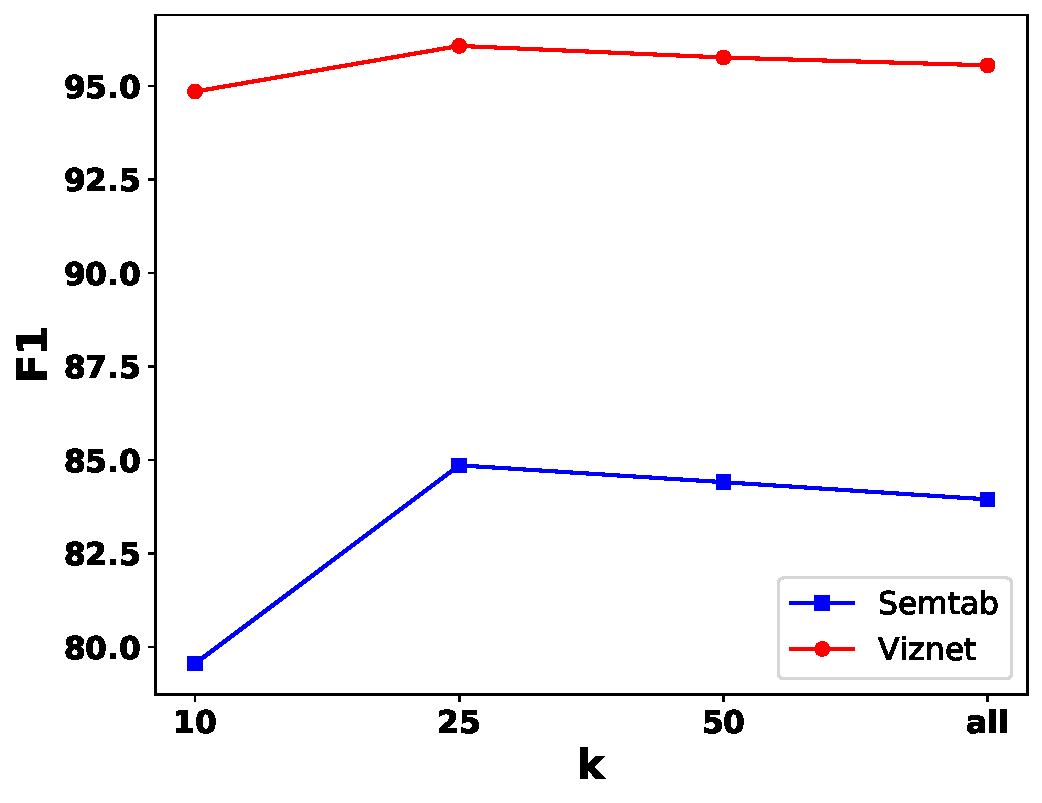
\includegraphics[width=\linewidth]{figures/kglink/F1_k.pdf}
\par\centering\small (a) Weighted F1
\end{minipage}\hfill
\begin{minipage}[b]{0.48\linewidth}
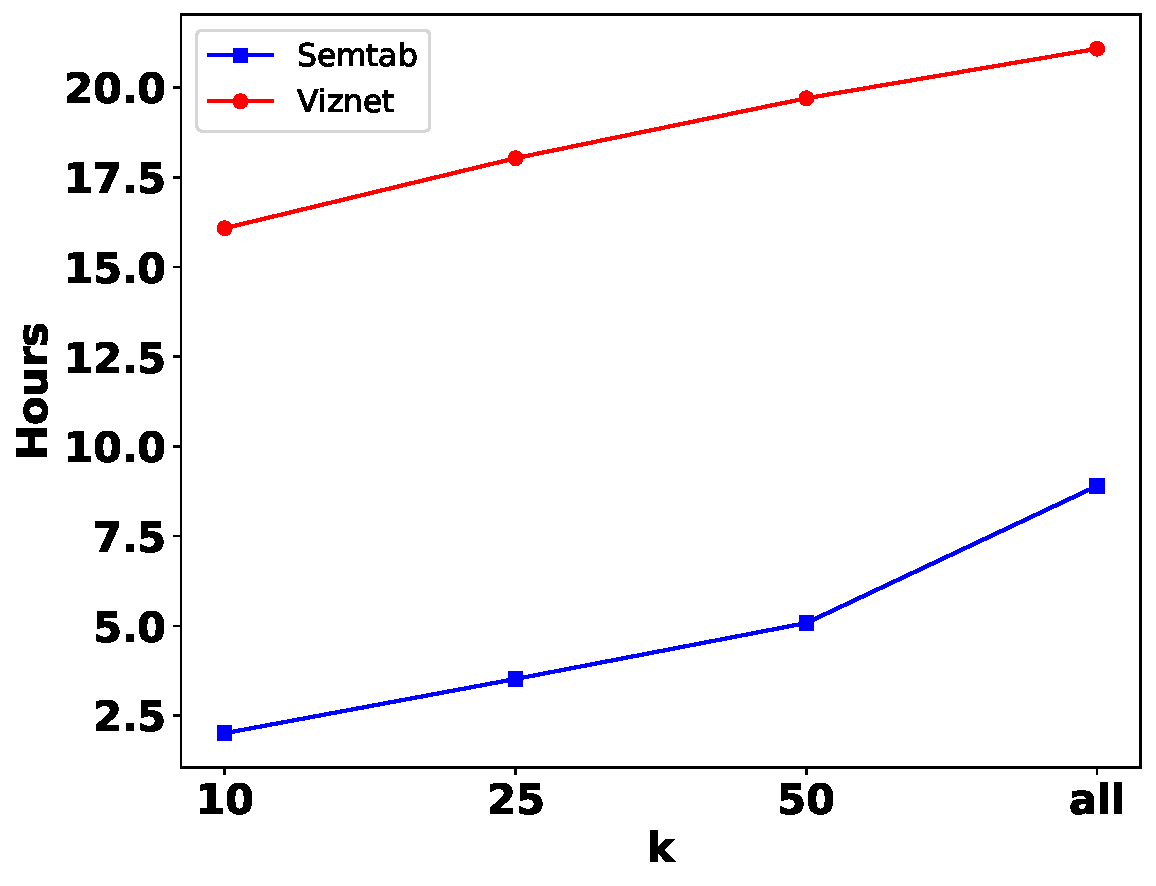
\includegraphics[width=\linewidth]{figures/kglink/k_time.pdf}
\par\centering\small (b) Time cost
\end{minipage}
\caption{Reported effect of the retained row budget $k$. The original two subfigures compare annotation quality and time cost on SemTab and VizNet. Reproduced from KGLink~\cite{kglink-publication}, Fig.~10.}
\label{fig:kglink:row-budget}
\end{figure}

The training-data study uses proportions $p=0.2,0.4,0.6,0.8,1.0$ while keeping the test set unchanged. It compares KGLink with the version without the representation-generation task. The experiment measures data efficiency by varying available supervision against a fixed evaluation set.

\subsection{Runtime in the Evaluated Configuration}
\label{sec:kglink:runtime}

Figure~\ref{fig:kglink:runtime} reproduces the original VizNet runtime chart. KGLink's reported training and inference times are 16.50 and 1.53 hours. The corresponding RECA values are 80.00 and 9.00 hours. The figure also shows methods with shorter measured times, including Doduo at 1.96 hours for training and 0.07 hours for inference. These measurements locate KGLink's annotation results within the costs of the evaluated implementations. Its use of external retrieval and a second training objective carries computation beyond the table encoder alone.

The chart labels MTab's inference entry as N/A. Training and inference times describe different preparation and prediction procedures. The comparison uses VizNet and the original experimental hardware.

The row-budget results address a separate resource decision. They vary how much table content is retained before encoding within KGLink, while the runtime chart compares complete methods. Reading the two studies together identifies the operational choice examined by the chapter. Graph relations determine which evidence enters the encoder, and the retained evidence has a measurable processing cost. The accuracy comparison therefore depends on the selected input and training configuration as well as on the availability of a knowledge graph.

\begin{figure}[tbp]
\centering
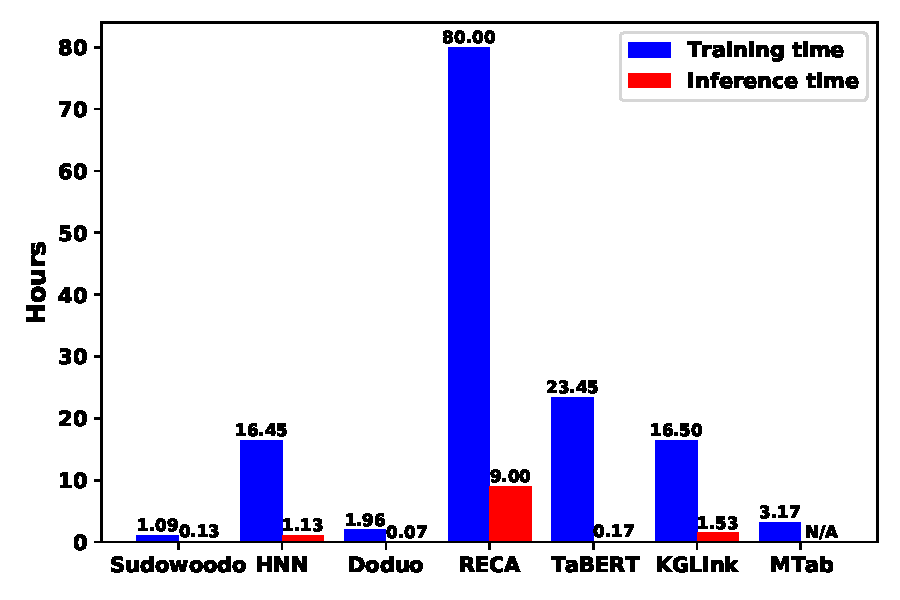
\includegraphics[width=0.9\linewidth]{figures/kglink/runtime.pdf}
\caption{Training and inference time reported on VizNet. Original image reproduced from KGLink~\cite{kglink-publication}, Fig.~7.}
\label{fig:kglink:runtime}
\end{figure}

\section{Discussion and Chapter Summary}
\label{sec:kglink:discussion}

KGLink uses explicit structure at two levels. Within a table row, graph neighborhood connections filter ambiguous entity candidates. Across the rows of a column, recurring graph neighbors support candidate-type selection. These operations determine what external text the encoder receives. The classifier then learns the relation between that evidence and a dataset's label vocabulary. The auxiliary representation task supplies an additional supervised connection between contextual evidence and the intended type description.

The empirical results support this division of responsibilities. The full BERT configuration improves on the version without the masked representation task and on the version without KG information. The row-selection comparison shows that choosing which table values enter the model changes the reported annotation scores. The no-linkage subset confirms that a trained model can continue to annotate tables when the graph stage supplies no retrieved evidence. Each observation corresponds to an explicit component or input condition in the architecture.

Knowledge coverage and annotation vocabulary remain material conditions. The graph-processing stage can use only entities and relations available to its linker and neighborhood retrieval. The supervised predictor learns the type set represented in training. The evaluated datasets use single-label column annotation and bounded table inputs. Those conditions determine the interpretation of the reported accuracy and weighted F1, including why a semantically reasonable graph description can still fail an exact-label evaluation.

The chapter answers the thesis's first research question by showing how graph-derived knowledge can augment a column representation while a learned model handles the target label granularity. The next chapter changes the evidence-maintenance problem. It studies classification when labels and observed examples arrive over successive rounds, using a task-specific graph to retrieve candidate labels and update the available evidence online.

% Working chapter, 2026-10-24. Author-confirmed publication-equivalent arXiv v4 compared; see evidence ledger.
% Evidence ledger: planning/verification-gorag.md. Do not designate this chapter final.
\chapter{Adaptive Graph Retrieval for Dynamic Classification with GORAG}
\label{ch:gorag}

This chapter is based on \emph{GORAG: Graph-based Online Retrieval Augmented Generation for Dynamic Few-shot Social Media Text Classification}, published in the Proceedings of the ACM Web Conference 2026~\cite{gorag-paper}. It studies the selection and maintenance of label evidence when a classification task acquires new classes over several rounds. The central question is how a language model can receive a query-specific candidate set while the evidence connecting text to labels changes over time.

\section{Dynamic Few-shot Classification}
\label{sec:gorag:task}

A classification label defines a decision that an application asks a model to make. When the application adds a more specific category, the decision changes even if the underlying language model stays fixed. For example, a social media classification task can initially distinguish threatening language and later introduce identity insults. A model must then distinguish the new label from earlier labels using the available annotated examples. The difficulty concerns both learning the meaning of a new category and keeping the current alternatives visible during prediction.

Few-shot classification supplies a small number of labeled examples for each class. Dynamic few-shot classification adds classes in successive rounds~\cite{gorag-xia-etal-2021-incremental}. The size of the label universe therefore grows independently of the number of examples available for each label. A retrieval system must update its evidence source as classes arrive, and each prediction must refer to the label set available at that round. This setting differs from repeatedly evaluating a fixed classifier on an unchanged collection of labels.

The task also exposes a limitation of simply placing more material in a language model's context. Additional examples provide information about labels, but a larger context can contain many examples that have little bearing on the current text. The candidate list itself grows as classes accumulate. Selecting text passages without narrowing the associated label alternatives leaves the model with a long classification instruction. GORAG therefore treats the selection of candidate labels as an explicit retrieval problem.

The index used in this chapter is a weighted graph of keywords and labels. A keyword can occur in examples from several classes. Its incident edges record these associations, and their costs distinguish how the term is represented in the indexed corpus. The graph allows several query keywords to be considered jointly. A label can participate in the connection between query keywords even when examining one keyword in isolation would give an ambiguous set of alternatives. The retrieved label set depends on the query terminals and the current graph.

GORAG also updates its index after classifying an unlabeled query. Keywords that were absent from the index can then become available to later queries. The predicted label associates the newly observed keywords with a class for subsequent retrieval. Support examples initialize the graph using their supplied labels.

The research question has three connected parts. First, how should a small support set become a graph whose edges distinguish keyword--label associations? Second, how should the graph select a different candidate set for each text as the label universe expands? Third, how can observations from previously classified texts enlarge the index? The following sections develop these operations and then examine their reported classification and resource results.

\begin{figure}[tbp]
\centering
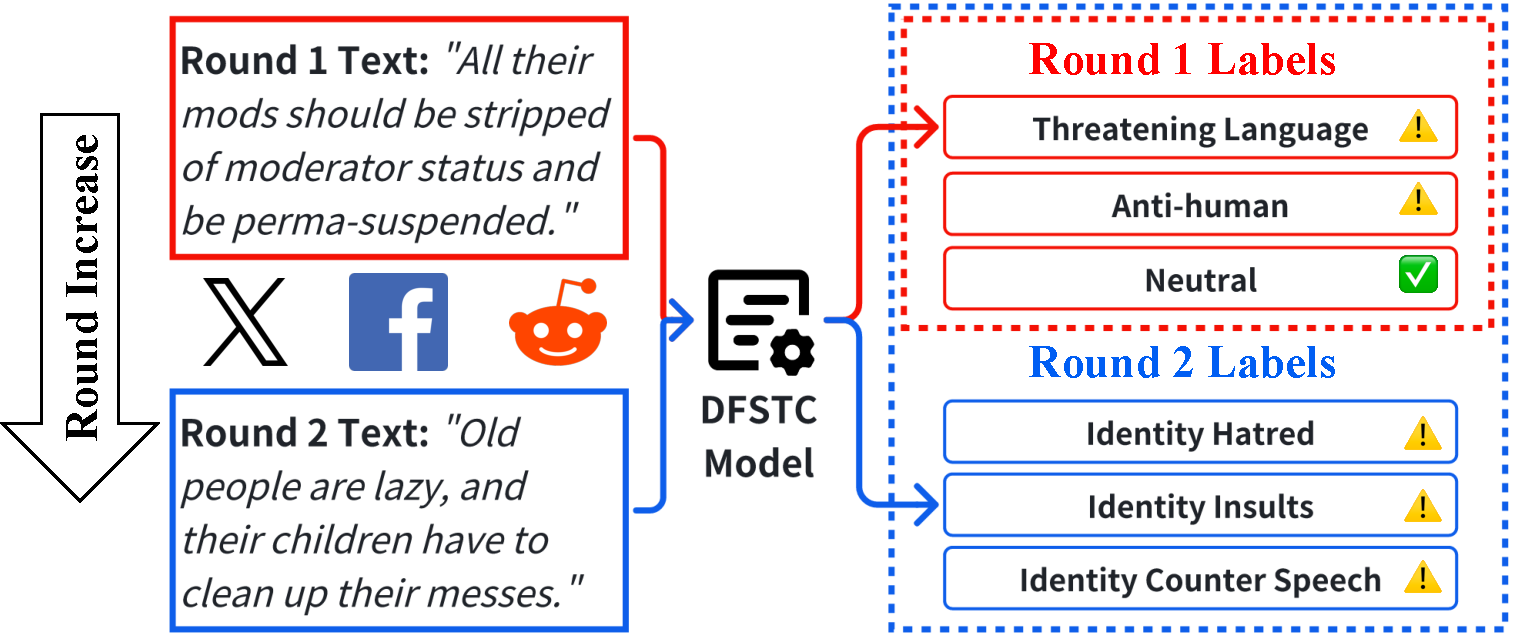
\includegraphics[width=0.9\linewidth]{figures/gorag/DFSTC_task.pdf}
\caption{Two rounds of the dynamic classification task. New abuse categories extend the available labels. Reproduced from Figure 1 of GORAG~\cite{gorag-paper}.}
\label{fig:gorag:task}
\end{figure}

\subsection{Rounds and information availability}
\label{sec:gorag:rounds}

Let $\mathcal{Y}_{\mathrm{new}}^r$ denote the labels introduced at round $r$. The current label universe is
\begin{equation}
\mathcal{Y}^r=\bigcup_{i=1}^{r}\mathcal{Y}_{\mathrm{new}}^i.
\label{eq:gorag:labels}
\end{equation}
The few-shot support data provide $k$ annotated texts per class, with $k$ equal to 1, 5, or 10 in the main experiments. A query text $t$ must be assigned a label from $\mathcal{Y}^r$. The superscript $r$ identifies the current classification round.

For clarity, the support collection visible at a round and the current query stream are separate objects. Support texts carry supplied labels. Query texts become visible as the system processes them, and their predictions can be used for subsequent index updates. Corpus statistics used in keyword scoring refer to training and query texts seen so far. The online association nevertheless inherits prediction errors when the classifier chooses an incorrect label.

Semantic label names supply another source of information. Where names are available, GORAG uses a language model to generate representative descriptions or keywords for labels. These descriptions enter the classification context, and label-derived keywords can support graph initialization. The zero-shot experiment later in this chapter uses this source without any labeled examples. It should therefore be read as a distinct initialization protocol rather than as a smaller support sample from the few-shot experiment.

\section{Weighted Graph Indexing}
\label{sec:gorag:indexing}

GORAG maintains an undirected weighted graph $\mathcal{G}^r=(\mathcal{V}^r,\mathcal{E}^r,\mathcal{W}^r)$. Its node set contains keyword nodes and label nodes. A keyword node represents an extracted word or short phrase. A label node represents a target class. The representation places label alternatives inside the same structure that stores their lexical associations. Support documents contribute keyword--label associations to this representation.

A keyword--label edge is introduced when a keyword occurs in a text associated with that label. Repeated occurrences across texts contribute to the edge weight. A keyword shared by several classes can therefore have several label neighbors, with a different cost for each association. Query retrieval will use these costs when choosing connections between mapped keywords. 

This representation separates the unit used to store evidence from the unit used to make the final prediction. The graph stores keyword--label associations. The language model receives the original query text as well as the retrieved alternatives and their descriptive information. The model can use syntactic and contextual information from the whole query even when retrieval has operated on a smaller collection of keywords. The keyword-only ablation examines the consequence of removing this full-text component.

\begin{figure}[tbp]
\centering
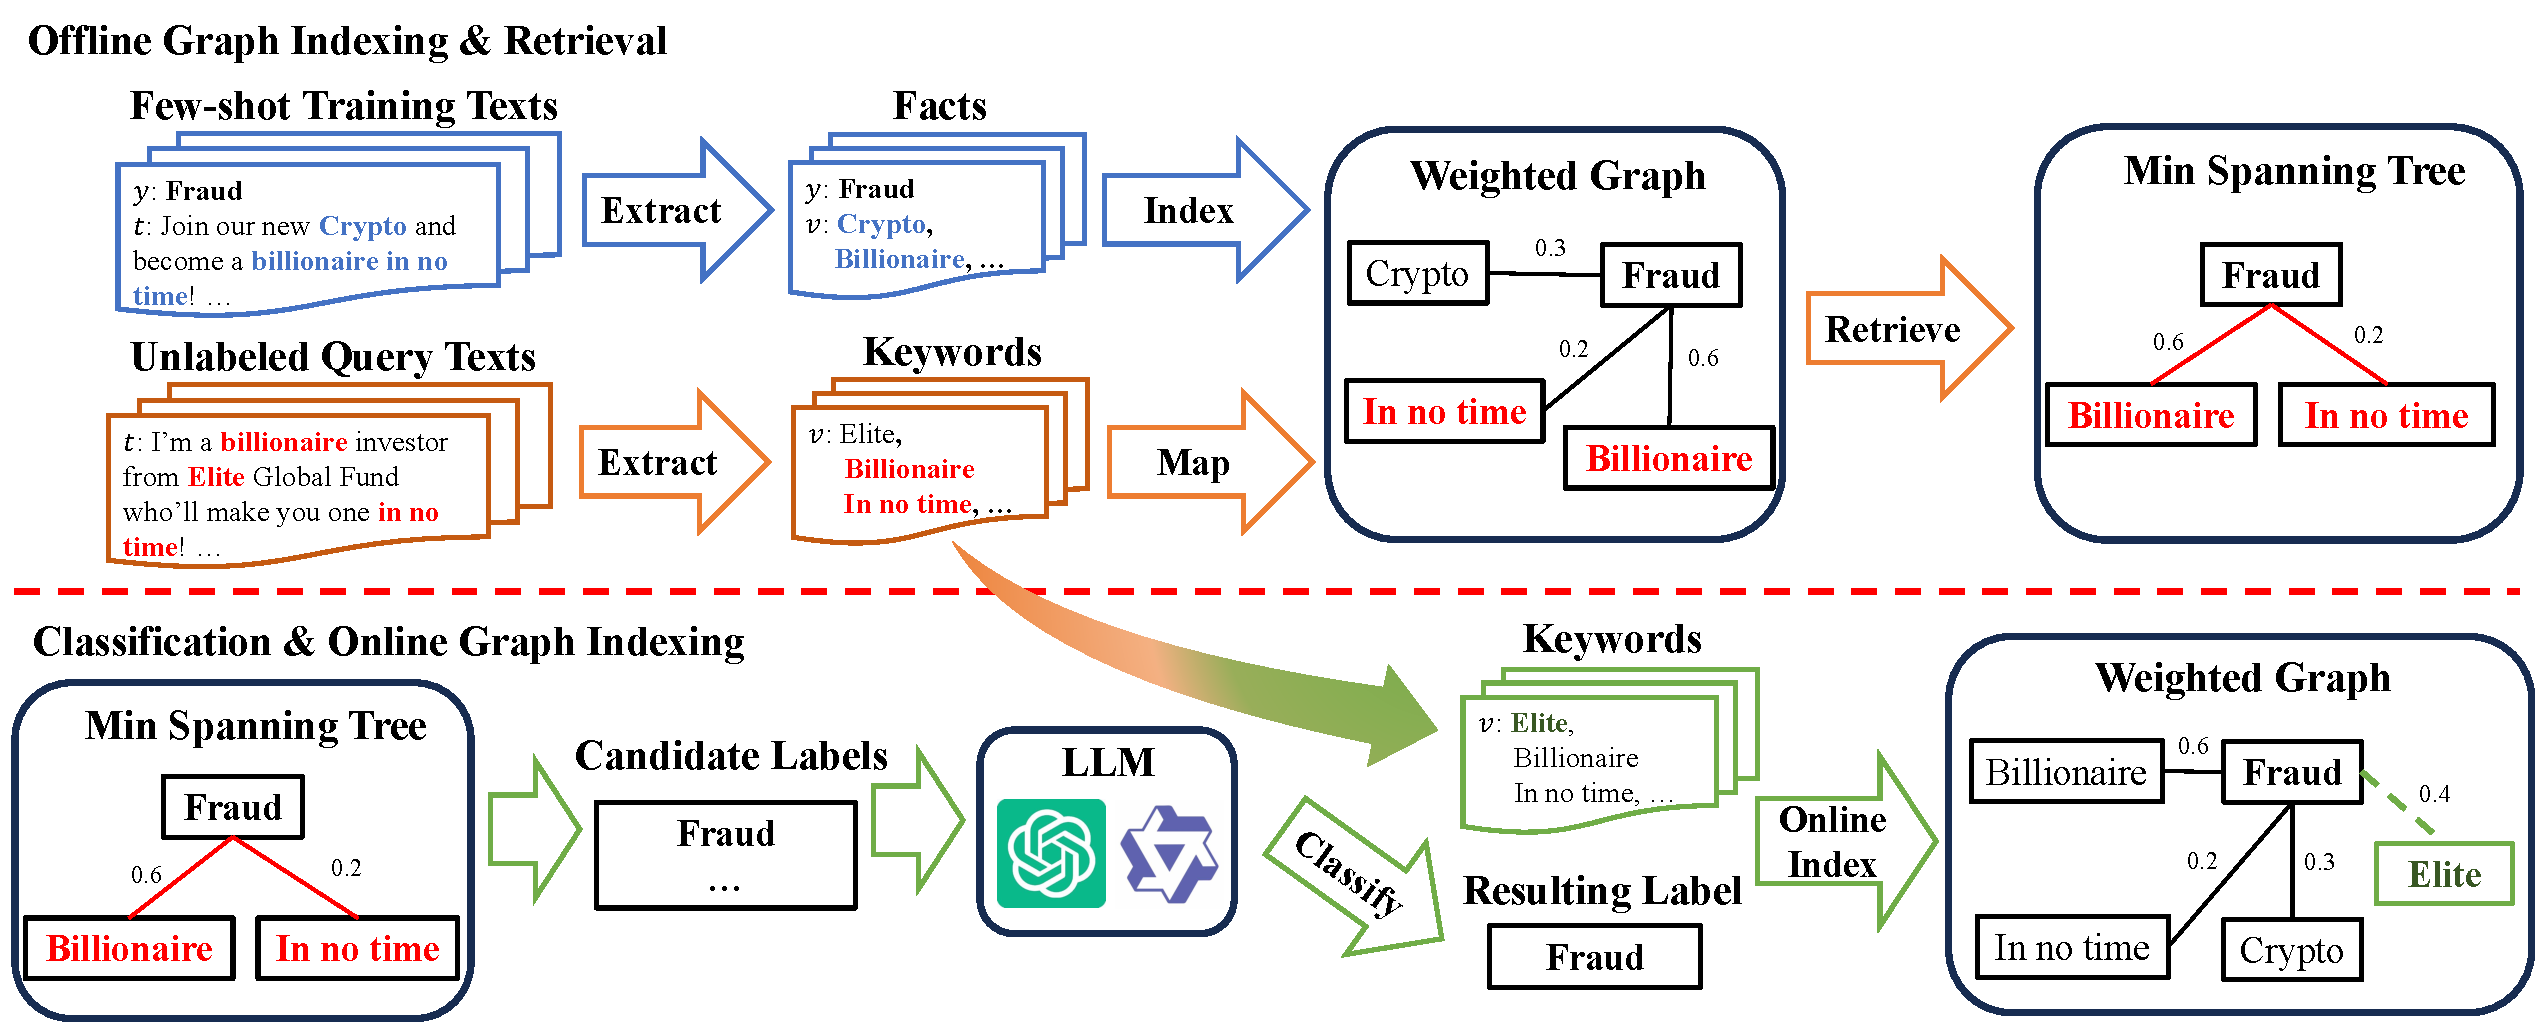
\includegraphics[width=\linewidth]{figures/gorag/GORAG_pipeline_example_new.pdf}
\caption{GORAG's offline indexing, query-dependent retrieval, classification, and online update. New query keywords are associated with the predicted class after classification. Reproduced from Figure 2 of GORAG~\cite{gorag-paper}.}
\label{fig:gorag:pipeline}
\end{figure}

\subsection{Keyword extraction and correlation scores}
\label{sec:gorag:keywords}

GORAG scores terms using normalized TF--IDF~\cite{gorag-tfidf}. Its extraction vocabulary includes words and phrases of fewer than three words. Let $\mathcal{T}_{\leq r}$ denote the corpus seen so far, and let $\operatorname{df}(v)$ be the number of its texts containing term $v$. The reported correlation score is
\begin{equation}
CS(v,t)=\frac{\operatorname{count}(v,t)}{|t|\log(|\mathcal{T}_{\leq r}|+1)}
\log\frac{|\mathcal{T}_{\leq r}|+1}{\operatorname{df}(v)+1}.
\label{eq:gorag:correlation}
\end{equation}
Here $\operatorname{count}(v,t)$ is the occurrence count of $v$ in $t$, and $|t|$ is text length. The expression combines frequency within the text with frequency across the observed corpus. Its corpus term changes when additional texts are observed. Terms with $CS(v,t)>\tau$ are retained, with $\tau=0.5$ in the original study. The method uses the score both to select keywords and to calculate association costs.
% Verification issue G5: source reports CS>tau with tau=0.5; normalization/threshold needs author/publication confirmation. Do not silently rescale.

A statistical extraction score gives each retained term a numerical contribution before graph retrieval. This contribution has a different role from the final language model's confidence in a label. The score determines which lexical units are indexed and how expensive their associations will be in retrieval. The evaluation of the full pipeline is therefore needed to establish the effect on classification.

Using short phrases can preserve a lexical combination that would be split by unigram indexing. At the same time, the extraction rule restricts what becomes a terminal later. Content absent from the extracted keyword set cannot directly act as a retrieval terminal for that query. The full query text remains available to the classifier, but its access to label evidence has already been shaped by the index representation. This relationship explains why extraction and classification should be described as separate stages.

\subsection{Keyword--label edge costs}
\label{sec:gorag:weights}

For keyword $v$ and label $y$, let $\mathcal{T}^{r,v,y}$ be the seen texts that contain $v$ and are associated with $y$. GORAG assigns the edge cost
\begin{equation}
w_{v,y}^r=\frac{\sum_{t_j\in\mathcal{T}^{r,v,y}}(1-CS(v,t_j))}{|\mathcal{T}^{r,v,y}|}.
\label{eq:gorag:weights}
\end{equation}
The complement converts a larger correlation score into a smaller contribution to connection cost. Averaging makes the edge depend on all contributing observations rather than on one occurrence. Offline observations use the supplied class of a support text; online observations use a predicted class when new query keywords are inserted.

An edge weight thus belongs to a particular keyword--label pair. It is not a global importance weight assigned to the keyword irrespective of class. The same keyword may occur in several label contexts, and the corresponding averages can differ. Retrieval uses the resulting cost structure together with connectivity. Replacing every cost by one preserves the graph's adjacency while removing this distinction, which is the purpose of the unit-weight ablation.

The averaging rule also identifies the granularity at which evidence is combined. Texts are not concatenated into one label description before the edge is scored. Each contributing text supplies a correlation value and the edge records their mean complement. A later text can contribute another occurrence to the associated pair. This design lets the index summarize recurrent lexical associations without putting every support text into each classification prompt.

\subsection{Merging label rounds}
\label{sec:gorag:merge}

At each round, the graph created from newly supplied information is merged with the graph accumulated from earlier rounds. The node and edge sets are unions. This operation retains the label universe already introduced while adding nodes and associations for the new task state. It differs from rebuilding a fresh graph containing only the most recently introduced labels, which would remove access to earlier alternatives.

GORAG also introduces edges between newly introduced and earlier label nodes. These bridges support connections between parts of the graph indexed in different rounds. Let $\mathcal{M}_y^r$ denote the keyword neighbors of label $y$. For a new label $y_n$ and an earlier label $y_o$, GORAG reports
\begin{equation}
w_{y_n,y_o}^r=\frac{1}{2}\left(
\frac{\sum_{v\in\mathcal{M}_{y_n}^r}w_{v,y_n}^r}{2|\mathcal{M}_{y_n}^r|}
+\frac{\sum_{v\in\mathcal{M}_{y_o}^r}w_{v,y_o}^r}{2|\mathcal{M}_{y_o}^r|}
\right).
\label{eq:gorag:labelbridge}
\end{equation}
The formula uses costs incident to both labels. These factors determine the relative cost of traversing a label bridge rather than a keyword association.
% Verification issue G6: preserve exact reported factors; source wording says weighted average.

Label bridges have a different evidential meaning from keyword--label edges. A keyword edge records a term's occurrence in texts associated with a class. A label bridge is added by the graph-merging procedure. It provides a connection through which retrieval can move between label regions. A retrieved path can therefore combine observed keyword associations with label bridges introduced during merging.

\section{Adaptive Candidate Label Retrieval}
\label{sec:gorag:retrieval}

For a query $t$, GORAG extracts keywords using the indexing procedure and partitions them according to whether they already occur in $\mathcal{V}^r$. Write these sets as $\mathcal{V}_{\mathrm{exist}}^t$ and $\mathcal{V}_{\mathrm{notexist}}^t$. The existing keywords become the terminals for current retrieval. The unseen keywords are held for online insertion after classification. The partition prevents the retrieval operation from treating an unindexed term as if it already had a known label neighborhood.

Retrieval seeks a low-cost connected structure that contains the mapped terminals. Label nodes encountered in this structure form the candidate set $\widehat{\mathcal{Y}}_t^r$. Connecting several terminals can select intermediate labels and keywords. The graph therefore determines the number of candidate labels through the returned structure, rather than requiring the same number of labels for all queries. A short query and a query containing several mutually distant indexed terms can produce different retrieval structures.

This terminal-connecting objective is related to the Steiner tree problem. In that problem, the required terminals are a subset of graph vertices, and the solution may use additional vertices to connect them. An ordinary minimum spanning tree instead spans all vertices of its input graph. These objects play distinct roles in GORAG's procedure. GORAG uses these intermediate structures to construct a heuristic connection among the query terminals.

\subsection{Tree and auxiliary-graph operations}
\label{sec:gorag:algorithm}

GORAG uses a greedy terminal-connecting procedure based on Mehlhorn's algorithm~\cite{gorag-mehlhorn1988faster}. The mapped keywords serve as terminals. An auxiliary graph $H$ represents connections between terminals, with edge weights given by path costs. A minimum spanning tree of $H$ selects a collection of terminal connections. Expanding these connections into their underlying paths produces the graph structure used for candidate selection. The language model then receives the labels encountered in this structure.

Once the expanded structure $S_t^r$ is obtained, the candidate set is
\begin{equation}
\widehat{\mathcal{Y}}_t^r=\mathcal{V}(S_t^r)\cap\mathcal{Y}^r.
\label{eq:gorag:candidates}
\end{equation}
Representative keywords and label descriptions are added to the classification prompt for the labels selected by this intersection.

\section{Classification and Online Indexing}
\label{sec:gorag:online}

GORAG constructs a classification input by concatenating the query text, extracted query keywords, retrieved candidate labels, and representative keywords associated with those labels. With $\mathcal{K}^t$ denoting query keywords and $\mathcal{K}_{\widehat{\mathcal{Y}}_t^r}$ the representative label information, the input is
\begin{equation}
c_t=\operatorname{Concat}\left(t,\mathcal{K}^t,\widehat{\mathcal{Y}}_t^r,\mathcal{K}_{\widehat{\mathcal{Y}}_t^r}\right).
\label{eq:gorag:context}
\end{equation}
A language model applies the classification instruction $p_{\mathrm{classify}}$ to this input and produces $y_t^*$. The graph narrows and describes the alternatives; the language model performs the final text classification.

Keeping the original query in this interface matters because keyword extraction removes ordering, local syntax, and surrounding discourse from the retrieval representation. The selected candidate set does not by itself determine how these features should affect the decision. The classifier can inspect the complete query alongside the retrieved label information. GORAG's keyword variant removes the full query from this input to test the contribution of that context under the same overall framework.

After the prediction, each keyword in $\mathcal{V}_{\mathrm{notexist}}^t$ is inserted into the graph and connected to $y_t^*$. The update can be written as
\begin{align}
\mathcal{V}^r&\leftarrow\mathcal{V}^r\cup\mathcal{V}_{\mathrm{notexist}}^t,\\
\mathcal{E}^r&\leftarrow\mathcal{E}^r\cup\{(v,y_t^*):v\in\mathcal{V}_{\mathrm{notexist}}^t\}.
\label{eq:gorag:update}
\end{align}
New associations receive weights through the reported weighting mechanism. Later queries can then map terms that were previously absent from the index. The update changes the retrieval source without fine-tuning the language model's parameters.

The prediction precedes insertion, so a new keyword's association can affect later queries but not the prediction that created it. Incorrect predicted labels can propagate through those associations. The offline ablation suppresses online expansion, measuring its contribution relative to an index that receives no such query-dependent additions.

\subsection{Computational organization}
\label{sec:gorag:computation}

The graph separates work performed at a label update from work performed for each query. Offline indexing processes the supplied texts, creates or updates keyword associations, generates label information when available, and merges the round's graph. The cross-round label bridges introduce interactions between the newly indexed and earlier label regions. In the source's abstract operation count, construction is expressed as
\begin{equation}
O\!\left(|\mathcal{Y}^r||\mathcal{Y}^{r-1}|+|\mathcal{V}_{\mathrm{new}}^r||\mathcal{D}^r|\right).
\label{eq:gorag:constructioncost}
\end{equation}
The two terms account for label merging and keyword--text processing. This count treats the associated text-processing and graph operations at the granularity used in that analysis. The number of tokens processed by a language-model call depends on the prompt and generated output, so the empirical token study supplies a separate measurement of model-facing work.

Per-query processing maps the extracted terms to the existing graph, obtains a connecting structure, builds the classification prompt, and inserts new terms after prediction. The index state can therefore grow during one round as well as between label rounds. Graph memory and prompt length measure different consequences of that growth. A larger stored index can provide more candidate associations while a query still receives only the labels selected by its own retrieval structure. The resource experiments report these two quantities separately.

\section{Experimental Design}
\label{sec:gorag:experiments}

The published study evaluates CAD, WOS, and IFS-Rel. CAD contains social media posts annotated for contextual abuse~\cite{gorag-vidgen2021introducing}. WOS contains academic texts associated with research-area labels~\cite{gorag-kowsari2017hdltex}. IFS-Rel supplies relation-classification examples derived from news text in an incremental few-shot benchmark~\cite{gorag-xia-etal-2021-incremental}. These datasets exercise different label vocabularies and text lengths within the dynamic classification setting.

The four-round split introduces 13 labels across CAD's rounds, 133 across WOS, and 64 across IFS-Rel. The test collections contain 817, 9,396, and 2,560 examples, respectively. IFS-Rel uses 40 test examples per label. Its balanced test allocation differs from the changing class frequencies in the other collections. Accuracy should therefore be interpreted with each dataset's actual split and distribution.

\begin{table}[tbp]
\centering
\caption{Dataset statistics for the four-round experiments, transposed from the original table. IFS-Rel has 40 test samples per label. Round label counts refer to newly introduced labels.}
\label{tab:gorag:dataset}
\small
\begin{tabular}{lrrr}
\hline
Statistic & CAD & WOS & IFS-Rel\\
\hline
Average text tokens & 154 & 200 & 105 \\
Round 1 test texts & 240 & 2,417 & 640 \\
Round 1 new labels & 4 & 32 & 16 \\
Round 2 test texts & 60 & 2,842 & 640 \\
Round 2 new labels & 3 & 53 & 16 \\
Round 3 test texts & 286 & 2,251 & 640 \\
Round 3 new labels & 3 & 30 & 16 \\
Round 4 test texts & 231 & 1,886 & 640 \\
Round 4 new labels & 3 & 18 & 16 \\
Total test texts & 817 & 9,396 & 2,560 \\
\hline
\end{tabular}
\end{table}


The label counts in Table~\ref{tab:gorag:dataset} describe labels introduced in each round. The classifier operates over their cumulative union. Thus the second WOS round adds 53 labels to the 32 labels already introduced, rather than replacing the earlier set by a new 53-label task. This distinction matters when relating the dataset statistics to the size of the classification instruction and to the graph state retained from earlier rounds.

The main few-shot study uses 1, 5, and 10 labeled examples per class. CAD and WOS RAG experiments use Qwen2.5-7B, while IFS-Rel uses GPT-4o. These are separate backbone conditions. The source reports an Intel Xeon Gold 5220R CPU at 2.20GHz and a single NVIDIA A100-SXM4-40GB GPU for the experiments. Runtime observations concern this implementation and hardware setting; API-backed inference also reflects the service used during the original study.

Classification accuracy requires an exact match between the model output and the ground-truth label name or number. An output that cannot be matched to the required class is not counted as correct. This protocol evaluates the final classification decision rather than a graded semantic similarity between arbitrary generated answers. A fluent explanation alone does not satisfy the metric.

\subsection{Compared methods and controls}
\label{sec:gorag:baselines}

The study compares six baselines. Entailment constructs text--label entailment pairs and fine-tunes a classifier~\cite{gorag-xia-etal-2021-incremental}. NaiveRAG retrieves text chunks from the indexed support information. Retrieved context is compressed by LongLLMLingua before classification~\cite{gorag-jiang-etal-2024-longllmlingua}. GraphRAG, LightRAG, and HippoRAG2 supply graph-based retrieval alternatives~\cite{gorag-edge2024local,gorag-guo2024lightrag,gorag-gutierrez2025memory}. Their classification results are measurements of the adaptations used in this study.

Entailment uses RoBERTa-large for five training epochs, a batch size of 16, a learning rate of $10^{-6}$, and Adam. LongLLMLingua is evaluated with compression rates of 0.75, 0.8, and 0.85, with 0.8 selected in the reported comparison. GraphRAG and LightRAG use local search. The source uses the nano-graphrag implementation for GraphRAG and NaiveRAG and the other baselines' official implementations. These choices identify the systems that produced the reported results.

The baseline collection tests several ways of allocating external context. NaiveRAG selects passages. LongLLMLingua changes which tokens remain in that context. The graph baselines select graph-associated information. GORAG explicitly selects labels through a connection structure and expands its lexical index online. These differences motivate the comparison, while the ablations isolate changes within GORAG's own pipeline more directly.

\section{Classification Results}
\label{sec:gorag:results}

The tables beginning with Tables~\ref{tab:gorag:main-wos} and~\ref{tab:gorag:main-ifs} preserve the WOS and IFS-Rel portions of the main accuracy table. Each dataset is split into one-, five-, and ten-shot tables, with rounds as columns. Each value is a fractional accuracy, and the labels available to the model expand with the round. The tables should be read by comparing methods under the same dataset, round, support size, and backbone.

% Layout split by shot; all 168 adopted WOS/IFS main cells retained.
\begin{table}[tbp]
\centering
\caption{WOS classification accuracy with one support example per label. Qwen2.5-7B is the RAG backbone. Values and emphasis reproduce the corresponding columns of GORAG's main table.}
\label{tab:gorag:main-wos}
\small
\begin{tabular}{lrrrr}
\hline
Method & Round 1 & Round 2 & Round 3 & Round 4\\
\hline
Entailment & {0.3695} & \underline{0.3994} & \underline{0.4510} & \underline{0.4030} \\
NaiveRAG & 0.3885 & 0.2267 & 0.1821 & 0.1653 \\
LongLLMLingua & 0.3806 & 0.2155 & 0.1770 & 0.1468 \\
GraphRAG & 0.3852 & 0.2213 & 0.1816 & 0.1641 \\
LightRAG & {0.3930} & 0.2202 & 0.1743 & 0.1625 \\
HippoRAG2 & \underline{0.4133} & 0.2552 & 0.2205 & 0.1906 \\
GORAG & \textbf{0.4866} & \textbf{0.4790} & \textbf{0.4736} & \textbf{0.4420} \\
\hline
\end{tabular}
\end{table}

\begin{table}[tbp]
\centering
\caption{WOS classification accuracy with 5 support examples per label. Qwen2.5-7B is the RAG backbone. Values and emphasis reproduce the corresponding columns of GORAG's main table.}
\label{tab:gorag:main-wos-5shot}
\small
\begin{tabular}{lrrrr}
\hline
Method & Round 1 & Round 2 & Round 3 & Round 4\\
\hline
Entailment & {0.3823} & \underline{0.4471} & \underline{0.4857} & \underline{0.4387} \\
NaiveRAG & {0.3904} & 0.2154 & 0.1475 & 0.1556 \\
LongLLMLingua & 0.3823 & 0.2202 & 0.1567 & 0.1382 \\
GraphRAG & 0.3897 & 0.2197 & 0.1770 & 0.1634 \\
LightRAG & 0.3806 & 0.2216 & 0.1767 & 0.1626 \\
HippoRAG2 & \underline{0.4245} & 0.2656 & 0.2210 & 0.1860 \\
GORAG & \textbf{0.4990} & \textbf{0.5109} & \textbf{0.4996} & \textbf{0.4717} \\
\hline
\end{tabular}
\end{table}

\begin{table}[tbp]
\centering
\caption{WOS classification accuracy with 10 support examples per label. Qwen2.5-7B is the RAG backbone. Values and emphasis reproduce the corresponding columns of GORAG's main table.}
\label{tab:gorag:main-wos-10shot}
\small
\begin{tabular}{lrrrr}
\hline
Method & Round 1 & Round 2 & Round 3 & Round 4\\
\hline
Entailment & {0.4187} & \underline{0.4222} & \underline{0.4787} & \underline{0.4442} \\
NaiveRAG & 0.3897 & 0.2187 & 0.1799 & 0.1649 \\
LongLLMLingua & 0.3901 & 0.2198 & 0.1608 & 0.1493 \\
GraphRAG & 0.3906 & 0.2219 & 0.1786 & 0.1625 \\
LightRAG & 0.3815 & 0.2145 & 0.1799 & 0.1632 \\
HippoRAG2 & \underline{0.4208} & 0.2666 & 0.2242 & 0.1915 \\
GORAG & \textbf{0.5134} & \textbf{0.5284} & \textbf{0.5234} & \textbf{0.4929} \\
\hline
\end{tabular}
\end{table}

\begin{table}[tbp]
\centering
\caption{IFS-Rel classification accuracy with one support example per label. GPT-4o is the RAG backbone. Values and emphasis reproduce the corresponding columns of GORAG's main table.}
\label{tab:gorag:main-ifs}
\small
\begin{tabular}{lrrrr}
\hline
Method & Round 1 & Round 2 & Round 3 & Round 4\\
\hline
Entailment & 0.3391 & {0.4008} & {0.3061} & {0.2971} \\
NaiveRAG & {0.7343} & 0.5394 & \underline{0.4719} & 0.5233 \\
LongLLMLingua & \underline{0.8750} & \underline{0.5734} & 0.4703 & \underline{0.5819} \\
GraphRAG & 0.6406 & 0.4406 & 0.3828 & 0.4297 \\
LightRAG & 0.7578 & 0.4906 & 0.3802 & 0.4531 \\
HippoRAG2 & 0.7313 & 0.4875 & 0.4297 & 0.4984 \\
GORAG & \textbf{0.9688} & \textbf{0.5938} & \textbf{0.4844} & \textbf{0.6165} \\
\hline
\end{tabular}
\end{table}

\begin{table}[tbp]
\centering
\caption{IFS-Rel classification accuracy with 5 support examples per label. GPT-4o is the RAG backbone. Values and emphasis reproduce the corresponding columns of GORAG's main table.}
\label{tab:gorag:main-ifs-5shot}
\small
\begin{tabular}{lrrrr}
\hline
Method & Round 1 & Round 2 & Round 3 & Round 4\\
\hline
Entailment & {0.6046} & {0.5516} & {0.4703} & {0.4395} \\
NaiveRAG & 0.7344 & 0.5406 & 0.4719 & {0.4938} \\
LongLLMLingua & \underline{0.8906} & \underline{0.5922} & \underline{0.4741} & 0.4903 \\
GraphRAG & 0.7813 & 0.4688 & 0.3734 & 0.4422 \\
LightRAG & 0.8281 & 0.5155 & 0.4010 & 0.4804 \\
HippoRAG2 & 0.7375 & 0.5016 & 0.4328 & \underline{0.5008} \\
GORAG & \textbf{0.9688} & \textbf{0.6172} & \textbf{0.4948} & \textbf{0.4988} \\
\hline
\end{tabular}
\end{table}

\begin{table}[tbp]
\centering
\caption{IFS-Rel classification accuracy with 10 support examples per label. GPT-4o is the RAG backbone. Values and emphasis reproduce the corresponding columns of GORAG's main table.}
\label{tab:gorag:main-ifs-10shot}
\small
\begin{tabular}{lrrrr}
\hline
Method & Round 1 & Round 2 & Round 3 & Round 4\\
\hline
Entailment & {0.5859} & \underline{0.5828} & {0.5193} & {0.4895} \\
NaiveRAG & 0.7406 & 0.5469 & 0.4688 & 0.5000 \\
LongLLMLingua & \underline{0.9219} & 0.5806 & \underline{0.5225} & \underline{0.5038} \\
GraphRAG & 0.8125 & 0.4719 & 0.3141 & 0.3922 \\
LightRAG & 0.8594 & 0.5156 & 0.4427 & 0.4610 \\
HippoRAG2 & 0.7406 & 0.4938 & 0.4438 & 0.4953 \\
GORAG & \textbf{0.9688} & \textbf{0.6250} & \textbf{0.5344} & \textbf{0.5469} \\
\hline
\end{tabular}
\end{table}


On WOS with one support example per label, GORAG reports accuracies of 0.4866, 0.4790, 0.4736, and 0.4420 across the four rounds. Entailment reports 0.3695, 0.3994, 0.4510, and 0.4030 in the same columns. The corresponding GraphRAG values are 0.3852, 0.2213, 0.1816, and 0.1641. These comparisons locate the result in a setting where the number of candidate labels increases substantially over the evaluation.

Additional support examples improve GORAG's WOS accuracy in the main table. At the fourth round, its one-, five-, and ten-shot values are 0.4420, 0.4717, and 0.4929. At the first round they are 0.4866, 0.4990, and 0.5134. The changing label universe and changing support size are separate experimental axes. 

IFS-Rel uses GPT-4o. In its first round, GORAG reports 0.9688 for all three support sizes, while the fourth-round scores are 0.6165, 0.4988, and 0.5469. The five-shot fourth-round value is below the one-shot value, so increasing support size does not produce a monotonic improvement in every setting. LongLLMLingua reports 0.5819, 0.4903, and 0.5038 in these fourth-round columns. HippoRAG2 reports 0.4984, 0.5008, and 0.4953; its five-shot result exceeds GORAG's five-shot result in that column.

CAD uses Qwen2.5-7B. Its GORAG first-round accuracy is 0.6125 in all three support settings. The fourth-round one- and five-shot accuracies are 0.3133 and 0.3146. Accuracy decreases in later rounds as the cumulative label set grows. 
% G2: full CAD table withheld from integrated chapter because source CAD/R4/10-shot is literal 03139. Exact working transcription in planning/gorag-working-cad-table.tex.

WOS improves with additional support in the displayed rounds, whereas IFS-Rel is non-monotonic across support sizes and CAD loses accuracy as labels accumulate.

\section{Ablations and Resource Use}
\label{sec:gorag:ablations}

The WOS ablation study uses a one-shot Qwen2.5-7B setting. The offline variant disables online indexing. The unit variant assigns cost one to every graph edge. The offline-and-unit variant removes both features. The keyword variant uses the extracted keywords in place of the complete query text for classification. These variants change specific inputs or index operations while retaining GORAG's overall classification task.

% Exact active-source transcription, numerical values retained.
\begin{table}[t]
	\centering
	\caption{Ablation experiments on WOS for GORAG's variants.}
	
	\label{tab:gorag:ablation}
	\small
		\begin{tabular}{l|l|c|c|c|c} 
			\hline\hline
			\multirow{2}{*}{\textbf{Dataset}} & \multirow{2}{*}{\textbf{Model}} & \multicolumn{4}{c}{\textbf{Round}}                                        \\ 
			\cline{3-6}
			& & R1              & R2         & R3           & R4  \\ 
			\hline
			\multirow{5}{*}{\textbf{WOS}} 
			& GORAG \textit{offline\&unit}          &     0.2979            &     0.2287            &       0.2645          &      0.2249                        \\
			& GORAG \textit{offline}          &     0.3063            &     0.2302            &       0.2455          &      0.2156                        \\
			&  GORAG \textit{unit}             & 0.4706          & 0.4394          & 0.4407          & 0.3899                      \\
			& GORAG \textit{keyword}         & \underline{0.4746}          & \underline{0.4606}          & \underline{0.4455}          & \underline{0.4030}             \\ 
			& \textbf{GORAG}                           & \textbf{0.4862}          &  \textbf{0.4649}              &     \textbf{0.4814}            &       \textbf{0.4210}                    \\
			\hline\hline
			
			
			
			
			
			
		\end{tabular}
	
\end{table}


In the ablation table, the full method reports 0.4862, 0.4649, 0.4814, and 0.4210 across rounds. The offline variant reports 0.3063, 0.2302, 0.2455, and 0.2156. The unit variant reports 0.4706, 0.4394, 0.4407, and 0.3899. Under this ablation protocol, removing online insertion has a larger observed effect than replacing the weighted graph with unit costs. This comparison concerns the variants reported together in that table.

The offline-and-unit variant reports 0.2979, 0.2287, 0.2645, and 0.2249. Its third- and fourth-round values exceed those of the offline variant. The effects of removing these components are therefore not strictly additive across rounds. The keyword variant reports 0.4746, 0.4606, 0.4455, and 0.4030, below the full method in each displayed column. The full query provides information useful to the classifier in these experiments even though keywords determine the retrieval terminals.

The publication gives different full-method values in the main and ablation WOS tables without explaining their provenance. Component comparisons here use the full-method row from the ablation table.

\subsection{Prompt tokens and graph growth}
\label{sec:gorag:resources}

The IFS-Rel one-shot token study reports average tokens per query and the corresponding US-dollar costs under the original study's pricing conditions. GORAG uses 557.5 tokens per query and reports a cost of \$0.004. The direct GPT-4o comparison uses 634.6 tokens and reports \$0.005. LongLLMLingua uses 2,771.3 tokens, NaiveRAG 4,537.4, LightRAG 7,866.3, and GraphRAG 9,296.3. Their reported costs are \$0.021, \$0.034, \$0.059, and \$0.070, respectively.

% Exact active-source transcription, numerical values retained.
\begin{table}[t]
	\centering
	\caption{Token cost on IFS-Rel dataset with 1-shot setting.}
	\label{tab:gorag:token}
	
	\small
		\begin{tabular}{l|c|c} 
			\hline\hline
			\textbf{Model} & \textbf{AVG Token per Query} & \textbf{AVG Cost per Query (USD)}  \\ 
			\hline
			GPT-4o         & 634.6                        & \$0.005                               \\
			LongLLMLingua  & 2771.3                       & \$0.021                               \\
			NaiveRAG       & 4537.4                       & \$0.034                               \\
			LightRAG       & 7866.3                       & \$0.059                               \\
			GraphRAG       & 9296.3                       & \$0.070                               \\
			\textbf{GORAG} & \textbf{557.5}               & \textbf{\$0.004}                      \\
			\hline\hline
		\end{tabular}
	
\end{table}


The token comparison measures how much context reaches the model in the evaluated implementation. GORAG's candidate-label representation uses fewer tokens than the listed retrieval baselines in this experiment. The historic dollar values provide the cost calculation reported with those measurements; they are not current API price quotations. Token totals and monetary costs should remain attached to this IFS-Rel one-shot protocol when discussing efficiency.

Graph growth is measured separately during the first IFS-Rel round with GPT-4o. The reported index contains 1,644 nodes and 1,771 edges at the 25-percent checkpoint, and 5,299 nodes and 5,503 edges at the final checkpoint. The corresponding reported memory values are 13.3 KB and 46.4 KB. These measurements concern the graph representation in that experiment. They do not include the complete memory required to host or serve the language model.
% G3: original intermediate node-count increment annotation is inconsistent; complete graph-growth table withheld pending clarification.

The original runtime study compares total time on WOS and CAD under the one-shot setting, using Qwen2.5-7B. Its figures belong to those dataset and hardware conditions. Online insertion adds work after each prediction, while statistical keyword indexing and smaller model inputs can change other parts of the pipeline. Runtime must therefore be measured end to end rather than inferred from token counts alone. This chapter retains the separation between prompt-token evidence, graph-memory evidence, and the source's total-time experiment.

\begin{figure}[tbp]
\centering
\begin{minipage}{0.48\linewidth}\centering
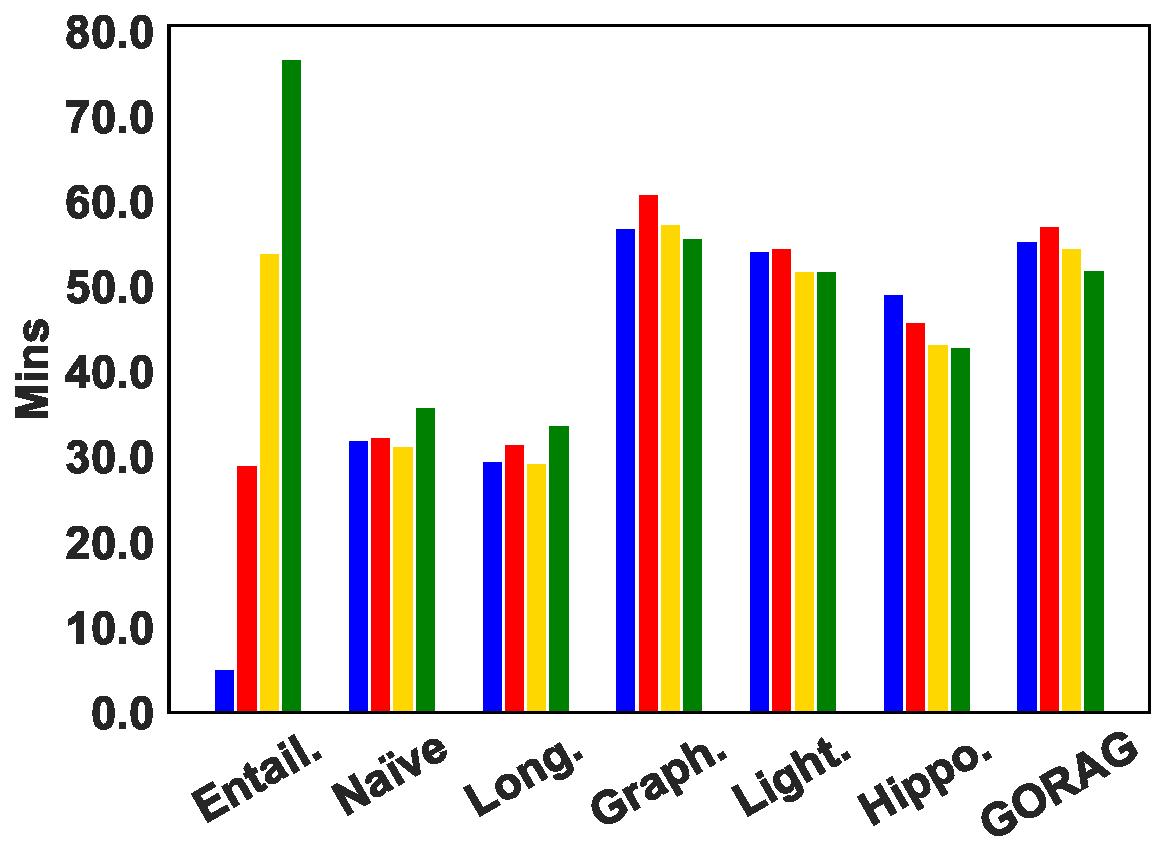
\includegraphics[width=\linewidth]{figures/gorag/runtime_wos.pdf}\par (a) WOS.
\end{minipage}\hfill
\begin{minipage}{0.48\linewidth}\centering
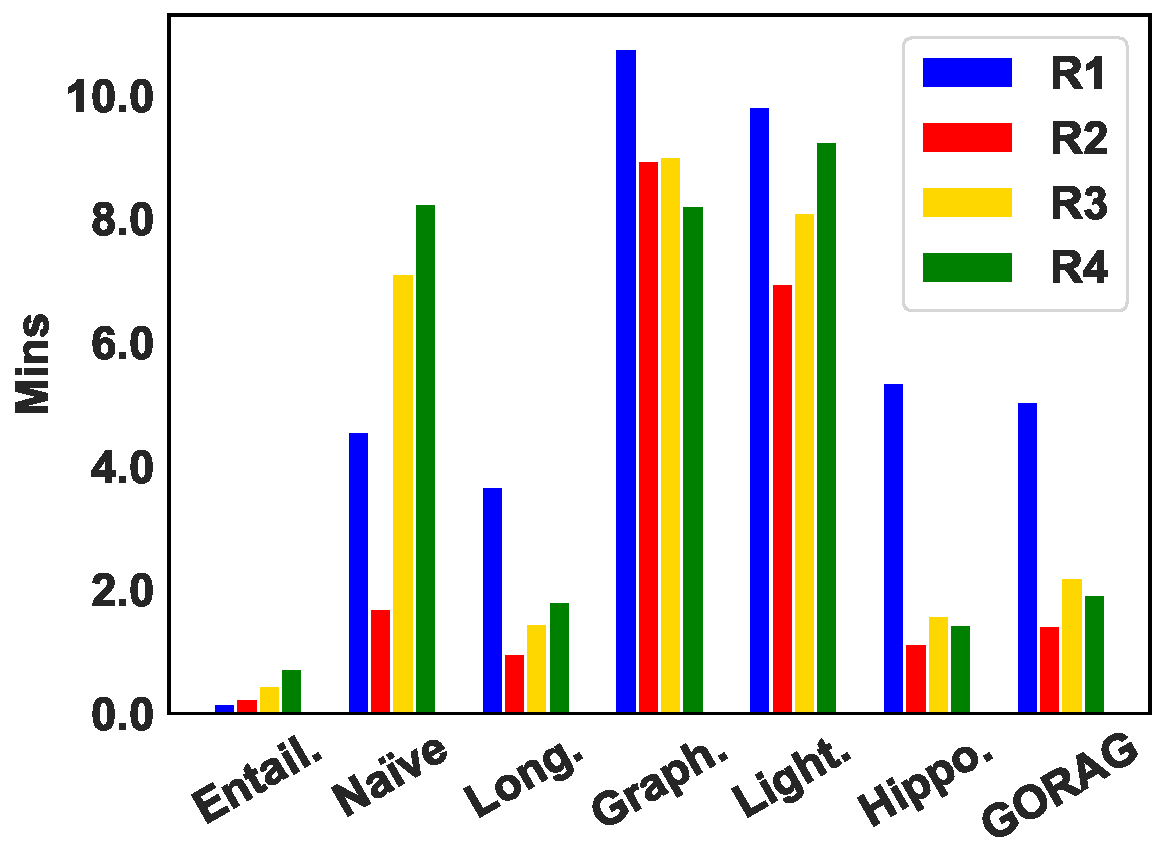
\includegraphics[width=\linewidth]{figures/gorag/runtime_cad.pdf}\par (b) CAD.
\end{minipage}
\caption{Total time in minutes for the one-shot four-round experiments with Qwen2.5-7B. The original R1--R4 legend in panel (b) applies to both panels. Reproduced from Figure 3 of GORAG~\cite{gorag-paper}.}
\label{fig:gorag:runtime}
\end{figure}

\section{Zero-shot and Round Generalization}
\label{sec:gorag:generalization}

The zero-shot IFS-Rel experiment supplies label names and language-model-generated descriptions without annotated support texts. GORAG extracts keywords from these descriptions to initialize its graph. The experiment consequently tests whether description-derived associations can support candidate selection and subsequent classification.

% Exact active-source transcription, numerical values retained.
\begin{table}[t]
	\centering
	\caption{0-shot experiments for GORAG and RAG baselines on IFS-Rel dataset under 0-shot setting.}
	\label{tab:gorag:zero}
	
	\small
		\begin{tabular}{l|c|c|c|c} 
			\hline\hline
			\textbf{Model}          & \textbf{R1}              & \textbf{R2}              & \textbf{R3}              & \textbf{R4}               \\ 
			\hline
			GPT-4o \cite{gorag-hurst2024gpt}                  & 0.9219                   & 0.5109                   & 0.4063                   & \underline{0.5936}                    \\ 
			LongLLMLingua \cite{gorag-jiang-etal-2024-longllmlingua}          & \underline{0.9281}                   & \underline{0.5297}                   & \underline{0.4234}                   & 0.5806                    \\
			LightRAG \cite{gorag-guo2024lightrag}                & 0.6718                   & 0.3047                   & 0.2135                   & 0.0977                    \\ 
			GraphRAG \cite{gorag-edge2024local}                & 0.5625                   & 0.1875                   & 0.1458                   & 0.0938                    \\
			\textbf{\textbf{GORAG}} & \textbf{\textbf{0.9328}} & \textbf{\textbf{0.5406}} & \textbf{\textbf{0.4375}} & \textbf{\textbf{0.6063}}  \\
			\hline\hline
		\end{tabular}
	
\end{table}


GORAG reports zero-shot accuracies of 0.9328, 0.5406, 0.4375, and 0.6063. The direct GPT-4o comparison reports 0.9219, 0.5109, 0.4063, and 0.5936. LongLLMLingua reports 0.9281, 0.5297, 0.4234, and 0.5806. The graph-based comparisons in the same table are lower under this initialization protocol. These values support the use of label descriptions as an initial retrieval source for this experiment.

The round-generalization study uses WOS split into four, six, and eight rounds under one- and five-shot settings. The displayed curve combines rounds one to four from the four-round split, rounds five and six from the six-round split, and rounds seven and eight from the eight-round split. These points represent results from different partitions of the label set. They do not form the trajectory of one index updated through eight consecutive rounds.

\begin{figure}[tbp]
\centering
\begin{minipage}{0.48\linewidth}\centering
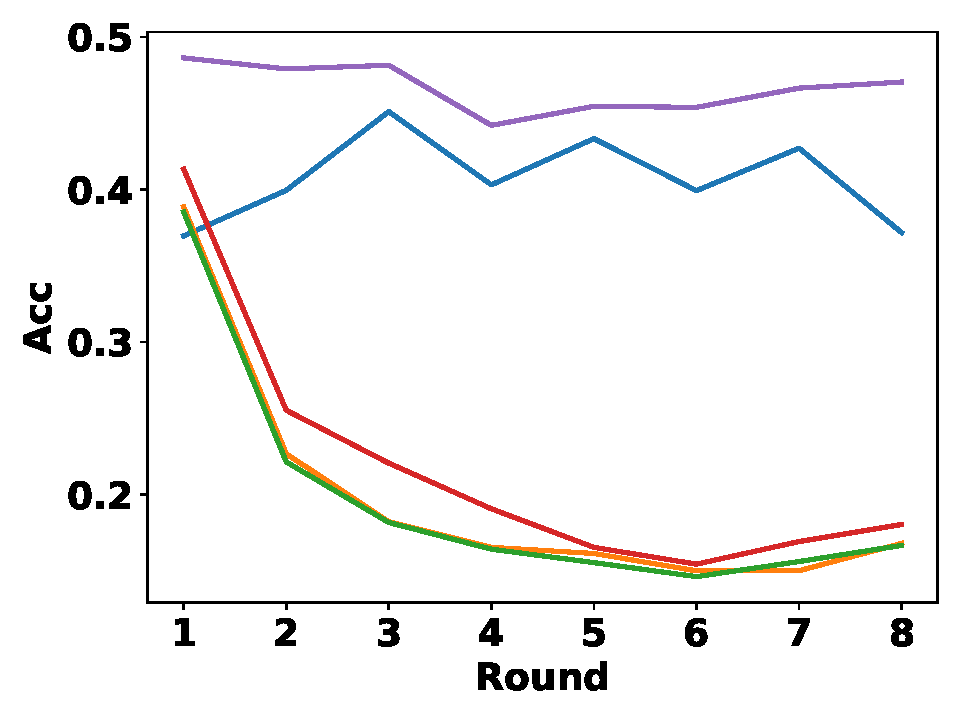
\includegraphics[width=\linewidth]{figures/gorag/wos_4_round_1.pdf}\par (a) One-shot.
\end{minipage}\hfill
\begin{minipage}{0.48\linewidth}\centering
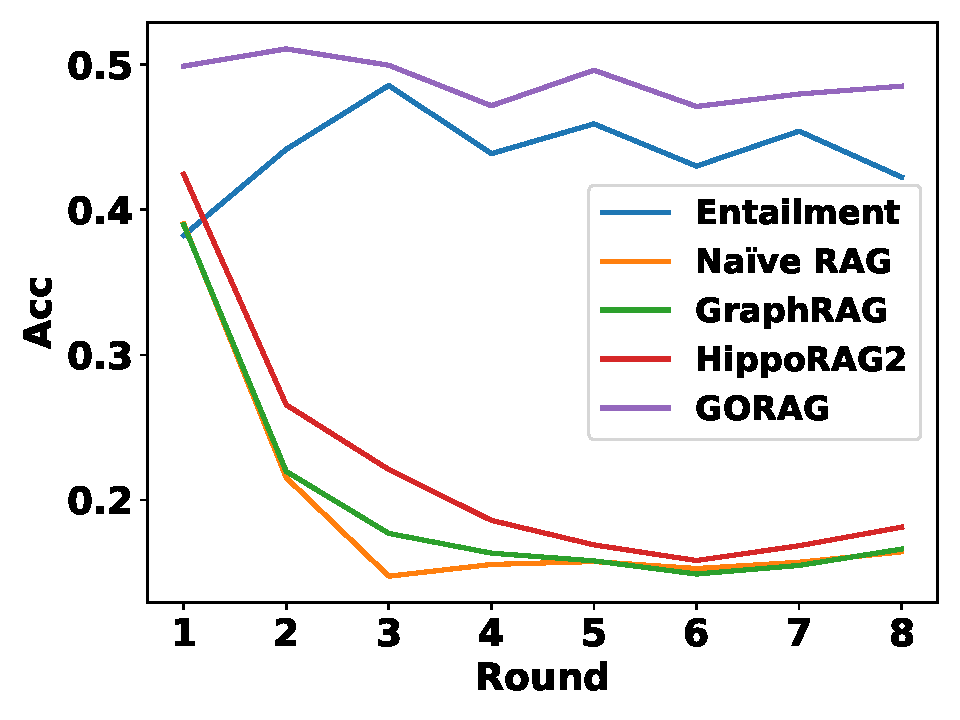
\includegraphics[width=\linewidth]{figures/gorag/wos_4_round_5.pdf}\par (b) Five-shot.
\end{minipage}
\caption{WOS classification across the reported round splits. Points 1--4 use the four-round split, 5--6 the six-round split, and 7--8 the eight-round split. The legend in panel (b) applies to both panels. Reproduced from Figure 4 of GORAG~\cite{gorag-paper}.}
\label{fig:gorag:rounds}
\end{figure}

\subsection{A retrieved classification case}
\label{sec:gorag:case}

Figure~\ref{fig:gorag:case} reproduces a contextual-abuse example from the original study. The query contains the terms highlighted in red. These terms map to keyword nodes, and the selected connecting structure passes through an insult label. The classifier outputs the abuse category shown in the figure. This example exposes the relationship between the extracted query evidence, the intermediate label node, and the final classification.

The useful property of the example is that candidate selection has a visible provenance. The label is connected to more than one term in the indexed representation. The displayed nonterminal neighbor also shows that a keyword neighborhood can contain more information than the connection chosen for the current text. Selecting a structure distinguishes the evidence used to connect the query terms from other associations present around the same label.

\begin{figure}[tbp]
\centering
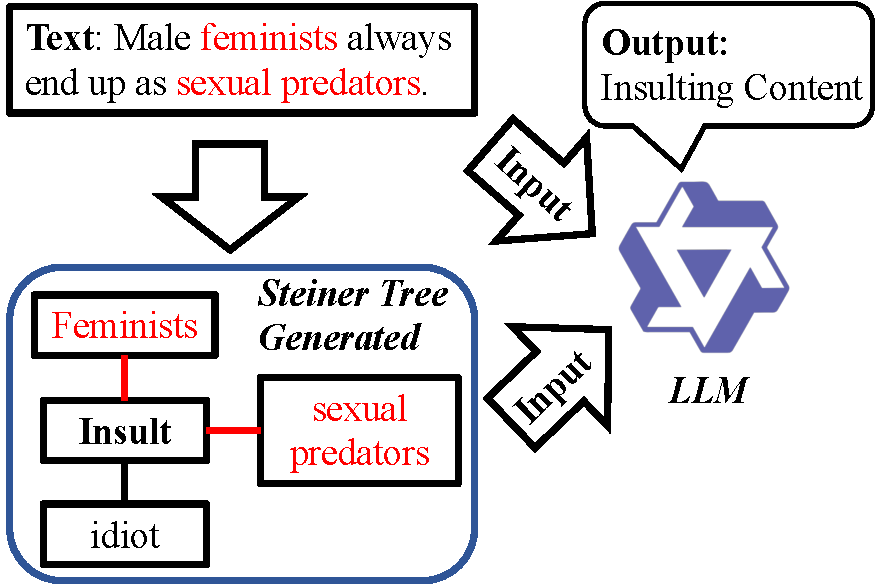
\includegraphics[width=0.75\linewidth]{figures/gorag/new_case.pdf}
\caption{A contextual-abuse example and its selected graph connections. Reproduced from Figure 5 of GORAG~\cite{gorag-paper}.}
\label{fig:gorag:case}
\end{figure}

\section{Discussion and Chapter Summary}
\label{sec:gorag:discussion}

GORAG places structure between the observation of text and the construction of a language model's classification instruction. Keywords connect the current text to an accumulated graph. Edge costs and terminal connections select a subset of label alternatives. The model then classifies the original text with these alternatives and their representative information. Structure serves as a task-specific evidence-selection mechanism.

The offline ablation shows the contribution of expanding the index beyond the support sample. Because these additions carry predicted labels, the method couples current classification with the evidence available to later queries.

The graph's paths provide a trace of the index connections used for retrieval. They can reveal which keywords and labels were linked by the selected structure. This trace explains the provenance of candidate selection in the constructed graph. The final classifier still receives text and makes a language-model prediction; the retrieved path is an external evidence object rather than an observation of the model's internal computation.

Several conditions bound the interpretation of the chapter's evidence. Keyword extraction determines which parts of a query can become terminals. Sparse support data and limited label descriptions determine initial coverage. Predicted-label insertion can add incorrect associations. The accuracy tables use exact label matching and different backbones for different datasets. Each condition identifies a concrete component or evaluation choice that affects the reported classification result.

Within these conditions, the study shows how a task graph can reduce the label-selection burden placed on a language model and maintain lexical evidence as the task evolves. The contribution differs from KGLink's use of an existing knowledge graph to enrich table representations. Here the structure is built and updated from task data, and its immediate output is a query-specific label set. The next chapter turns from choosing among labels to selecting connected textual facts for an open-ended answer. That change requires a retrieval objective that accounts for the relevance and connection cost of evidence beyond a fixed classification vocabulary.

\chapter{Connected Evidence Selection for Language Models with AGRAG}
\label{ch:agrag}

This chapter is based on \emph{AGRAG: Advanced Graph-based Retrieval-Augmented Generation for LLMs}, published at ICDE 2026~\cite{agrag-paper}. It studies how a retrieval system can select connected evidence and communicate the relationships among retrieved facts to a language model. The task extends beyond retrieving a relevant label. An answer may require several facts, their connections, and the surrounding passages that explain them.

\section{Research Problem and Evidence Requirements}
\label{sec:agrag:problem}
A retrieval system can locate passages relevant to a question while still leaving the generator with the task of discovering how those passages fit together. This distinction matters when a question asks for a summary, an explanation, or a response that combines information from different parts of a corpus. Similar passages may repeat one fact. Passages containing different parts of an answer may share few words. A graph provides an explicit representation of these connections, but the system must still decide which part of the graph to supply to the generator.

The research question in this chapter is how to select evidence that combines query relevance with connectivity. There are two related decisions. The first concerns the construction of the graph from text. Extracted entities establish the vocabulary over which subsequent retrieval operates. The second concerns the subgraph returned for a query. A ranking of individual nodes assigns relevance scores, whereas a connected subgraph also specifies relationships among the selected items. AGRAG addresses these decisions through statistical entity extraction, influence-aware graph retrieval, and a separate hybrid passage retrieval channel.

Consider a corpus containing statements about an illness, the organ that it affects, and the routes through which it spreads. A query may match facts mentioning the illness and the organ. Connecting those facts can identify a small initial structure, but answering the question may require a neighboring fact that specifies another anatomical component. The original example in Figure~\ref{fig:agrag:example} illustrates this distinction. The example motivates expansion beyond an initial terminal-connecting structure. 

The input is a text corpus $\mathcal{T}$ and a natural-language query $q$. The corpus is divided into chunks $\mathcal{T}_c$. The indexed graph $\mathcal{G}=(\mathcal{V},\mathcal{E})$ contains entity nodes, passage nodes, and several kinds of edges. Query processing identifies an initial set of relevant triple facts, assigns node influence scores and edge costs, and produces a subgraph for generation. A hybrid retriever supplies additional passages from the same corpus. The output is an answer conditioned on the query, a textual serialization of the retrieved graph, and the hybrid passages.

The evidence representation has two levels. Entity and relation information expresses specific connections. Passage nodes preserve links to the text from which those connections were extracted. The graph serialization gives the generator a relational account of the retrieved material, while passages provide the language surrounding those facts. This division is central to AGRAG. A retrieved graph may identify the relevant relationship without preserving every qualification or explanatory detail in a paragraph. The hybrid channel supplies contextual material alongside the graph.

The chapter evaluates the resulting pipeline on tasks with different answer requirements. Fact retrieval emphasizes individual facts. Complex reasoning combines facts. Contextual summarization requires coverage of several evidence items. Creative generation evaluates responses grounded in retrieved material while allowing more flexible output. Text classification supplies a further setting in which graph retrieval identifies candidate labels. Each task retains its own evaluation protocol, so the results are interpreted by task rather than combined into a single measure of reasoning.

\section{Framework and Graph Construction}
\label{sec:agrag:construction}
\subsection{The three-stage pipeline}
AGRAG separates data preparation, graph retrieval, and hybrid retrieval. Data preparation builds the graph and the passage indexes. Graph retrieval conditions the graph on a query through semantic mapping and influence scores, then selects a connected evidence subgraph. Hybrid retrieval combines dense passage similarity with BM25. Figure~\ref{fig:agrag:pipeline} reproduces the original architecture.

\begin{figure}[tbp]
\centering
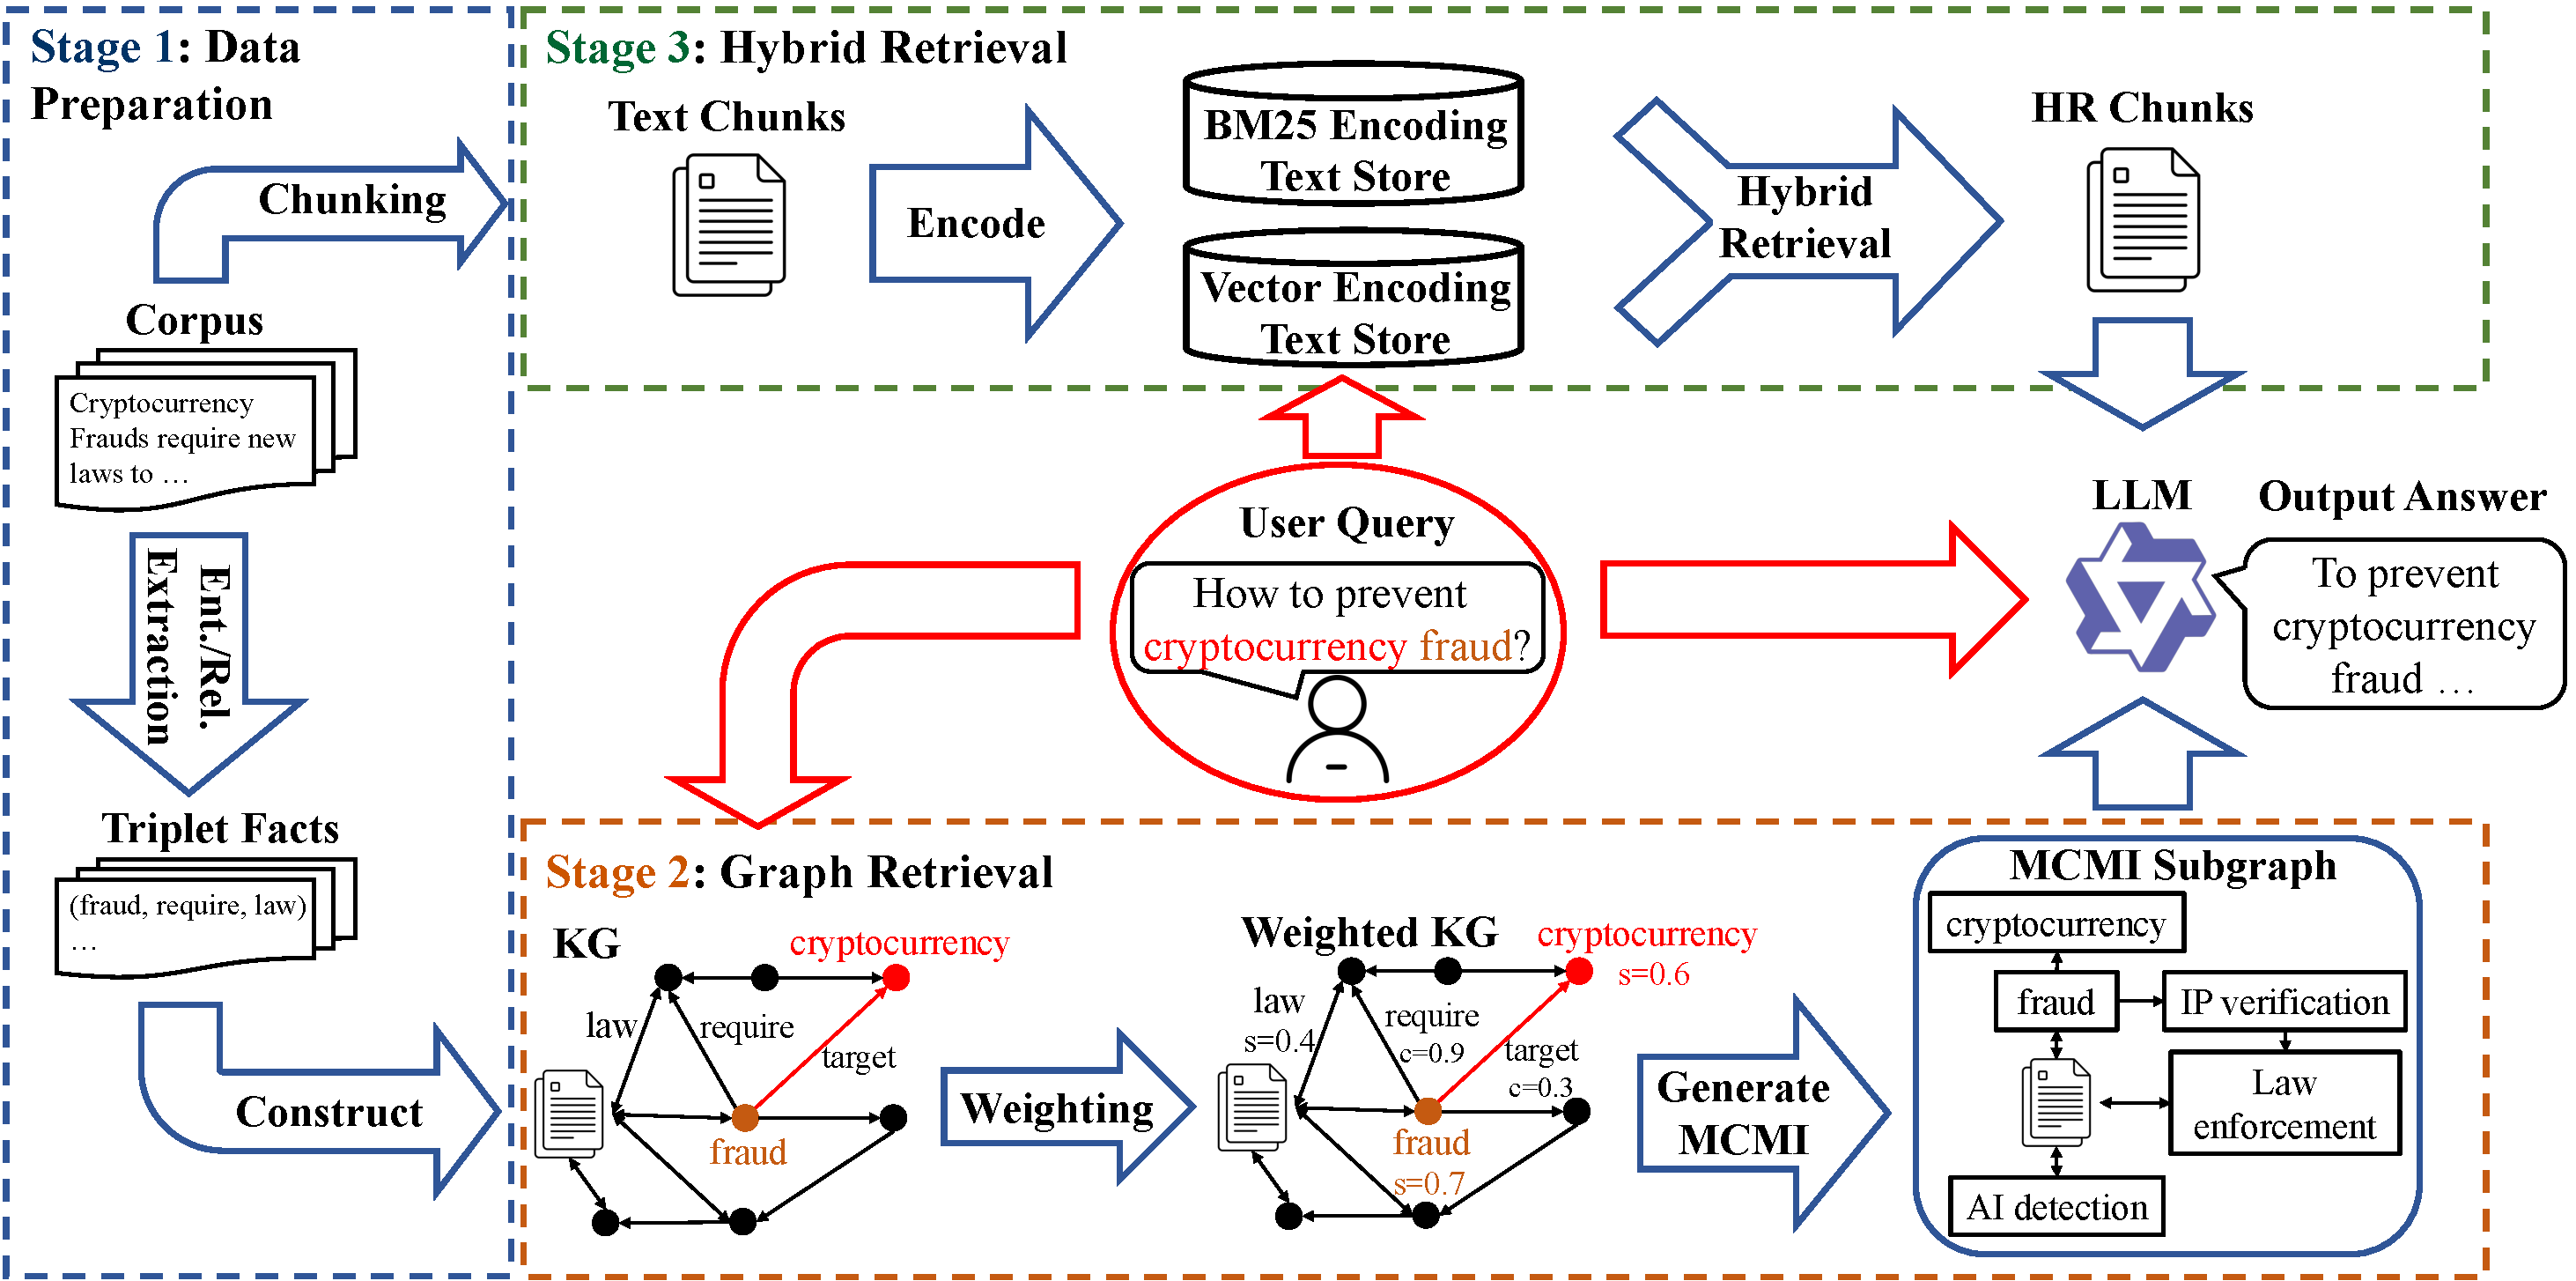
\includegraphics[width=\textwidth]{figures/agrag/AGRAG_pipeline.pdf}
\caption{The AGRAG pipeline. The original figure separates corpus preparation, query-conditioned graph retrieval, and hybrid passage retrieval. Reproduced from Figure 1 of the source paper~\cite{agrag-paper}.}
\label{fig:agrag:pipeline}
\end{figure}

The stages have different update requirements. Chunking, entity extraction, relation extraction, and the construction of passage links belong to corpus indexing. Mapping a query to graph facts, computing its influence scores, and expanding its evidence subgraph occur during query processing. Dense and sparse passage indexes support the hybrid channel. This organization identifies which costs arise from preparing the corpus and which recur for each query.

The statistical component replaces the entity extraction step used in the compared graph pipelines. Language models remain involved in relation extraction, filtering raw mapped triples, and generating answers. The entity-extraction ablation changes the nodes supplied to subsequent relation extraction and retrieval.

\subsection{Chunking and statistical entity extraction}
The corpus is split into overlapping text chunks,
\begin{equation}
\mathcal{T}_c=\operatorname{Split}(\mathcal{T},l_t,l_o),
\label{eq:agrag:chunking}
\end{equation}
where $l_t$ is the chunk length and $l_o$ is the overlap. The reported main setting uses 256 tokens per chunk and an overlap of 32 tokens. Overlap allows adjacent chunks to share text at their boundaries; the graph subsequently connects chunks through the entities they contain.

AGRAG considers words and phrases up to a maximum n-gram length $b$. For a candidate term $v$ in chunk $t$, the extraction rule modifies TF--IDF~\cite{agrag-tfidf} to define the score
\begin{equation}
\operatorname{ER}(v,t)=
\frac{\operatorname{count}(v,t)}{|t|\log(|\mathcal{T}_c|+1)}
\log\frac{|\mathcal{T}_c|+1}{|\{t_j\in\mathcal{T}_c:v\in t_j\}|+1}.
\label{eq:agrag:extraction-score}
\end{equation}
The first factor depends on within-chunk frequency and length. The second distinguishes terms according to their distribution across chunks. The extracted set is
\begin{equation}
\mathcal{V}_t=\{v:\operatorname{ER}(v,t)>\tau\},
\label{eq:agrag:entities}
\end{equation}
with maximum n-gram length $b$ and threshold $\tau$ controlling candidate boundaries and selection. The main paper reports $b=3$ and $\tau=0.5$.

The extraction rule uses terms appearing in the corpus. This constrains the origin of entity strings and makes their relationship to the indexed text explicit. Its decisions are based on term statistics, so linguistic salience and factual importance need not coincide. A frequently mentioned generic term and a rare but relevant phrase have different statistical profiles. The sensitivity experiment therefore examines both the phrase boundary and the extraction threshold.

An entity string identifies a graph node, while its occurrences connect that node to passages. This provides a path from fine-grained graph retrieval back to textual evidence. A shared entity can also connect information across chunks. The utility of these connections depends on whether the extracted string captures the intended entity and whether occurrences have compatible meanings. The evaluation measures the complete retrieval and generation pipeline under the reported extraction settings.

\subsection{Relations, passage nodes, and synonyms}
For each chunk, the language model receives the selected entity set and the chunk text, and extracts relations,
\begin{equation}
\mathcal{E}_t=\operatorname{LLM}(\mathcal{V}_t,t,p_{\mathrm{re}}).
\label{eq:agrag:relations}
\end{equation}
The prompt $p_{\mathrm{re}}$ asks for relations between the extracted entities in the chunk. The resulting entity--relation--entity triples provide the graph's factual edges. The statistical stage and the model stage therefore operate consecutively: one selects entity candidates from observed terms, and the other supplies relations conditioned on those candidates and their context.

Chunks are also inserted as passage nodes. A \textit{Contains} edge connects a passage to an entity extracted from it. These links preserve the association between the symbolic representation and the source chunk. They also allow paths to cross passages through shared entities. A passage contributes contextual evidence to graph retrieval without being reduced to a single isolated fact.

The graph includes synonym edges between entity nodes whose embedding similarity exceeds a threshold $\varphi$. Such an edge expresses an embedding-based correspondence between strings. It permits retrieval to connect different expressions that would otherwise form separate nodes. Its role differs from an extracted relation: an extracted relation comes from the language model's reading of a chunk, whereas a synonym edge comes from a similarity test. Both affect graph connectivity, and both remain part of the retrieval conditions.

AGRAG additionally introduces a pseudo node linked to passage nodes. The reported cost of each pseudo edge is 10. This connection gives the graph a route between otherwise disconnected portions while penalizing its use relative to semantically relevant factual edges. The pseudo connection is a connectivity device, so it should be distinguished from a factual assertion in the source corpus when interpreting the retrieved structure.

\section{Query Mapping and Influence-aware Retrieval}
\label{sec:agrag:influence}
\subsection{Mapping a query to triple facts}
At query time, AGRAG first identifies facts that are semantically close to the query. A text encoder $\mathcal{M}$ maps the query and a textual rendering of each triple to vectors. With $\mathbf{q}=\mathcal{M}(q)$ and $\mathbf{f}=\mathcal{M}(f)$, the mapping score is
\begin{equation}
\operatorname{MS}(\mathbf{q},\mathbf{f})=
\cos(\mathbf{q},\mathbf{f}).
\label{eq:agrag:mapping}
\end{equation}
The highest-scoring $k_a$ facts form the raw mapped set $\mathcal{F}_{\mathrm{raw}}$. The main setting uses $k_a=5$. This stage locates candidate facts in the indexed graph before graph propagation begins.

A model-based filtering step then evaluates the raw facts with respect to the query,
\begin{equation}
\mathcal{F}=\operatorname{LLM}(\mathcal{F}_{\mathrm{raw}},q,p_{\mathrm{tf}}).
\label{eq:agrag:filter}
\end{equation}
The filtered set $\mathcal{F}$ defines the query anchors. Dense mapping and filtering play different roles. Dense mapping produces a short candidate list efficiently. Filtering evaluates the candidates jointly with the actual query. The filtering ablation removes the second operation and tests its contribution to answer quality and cost.

The anchors determine where graph retrieval starts. They do not themselves specify the complete answer context. Facts connecting or surrounding the mapped set can be useful even when their direct similarity to the query is lower. Graph influence provides a way to score these surrounding items using their connection to the mapped facts. Edge costs then retain a separate measure of semantic relevance during subgraph construction.

\subsection{Node influence and edge costs}
AGRAG uses a personalized PageRank-style propagation~\cite{agrag-haveliwala2002topic} to assign query-dependent influence scores,
\begin{equation}
\mathbf{s}=\lim_{i\rightarrow\infty}\mathbf{s}^{(i)},\qquad
\mathbf{s}^{(i)}=(1-d)\mathbf{p}+d\mathbf{P}\mathbf{s}^{(i-1)}.
\label{eq:agrag:propagation}
\end{equation}
Here $\mathbf{p}$ is determined by nodes associated with the filtered mapped facts, and $\mathbf{P}$ is the graph propagation matrix specified in the source. The reported setting uses $d=0.5$ and stops the iteration when the change is below $10^{-7}$. The score of a node $v$ is $s_v=\mathbf{s}[v]$. Passage-node scores are multiplied by 0.05 to balance their contribution relative to entity nodes.

The personalization entries identify nodes participating in the mapped facts: an anchored node receives entry one and the other nodes receive zero. The graph operator is specified by
\begin{equation}
\mathbf{P}[u][v]=
\begin{cases}
1/|\mathcal{N}(u)|,&(u,v)\in\mathcal{E},\\
1/|\mathcal{V}|,&\text{otherwise}.
\end{cases}
\label{eq:agrag:graph-operator}
\end{equation}
Nonadjacent node pairs receive the constant term in this operator. The recurrence uses this matrix with the damping value in Equation~\ref{eq:agrag:propagation}, followed by passage-node scaling.

The node score is computed before neighborhood expansion. Consequently, a candidate's influence refers to its position in the indexed graph under the query anchors. The subgraph selection procedure uses these assigned scores as it changes which edges and nodes are included. This distinction separates propagation over the evidence source from expansion of the context returned to the model. The former establishes a score landscape; the latter selects an evidence structure using that landscape and the semantic edge costs.

Influence and direct similarity answer different retrieval questions. Similarity asks how closely a triple's wording corresponds to the query. Influence additionally depends on graph connectivity to query anchors. A node can receive influence through connections to several mapped facts. The subgraph selection stage uses these scores alongside edge costs so that the retrieval decision reflects both kinds of information.

For an edge $e=(u,v)$ associated with fact $f_e$, AGRAG defines
\begin{equation}
c_e=\frac{1-\operatorname{MS}(\mathbf{q},\mathbf{f}_e)}{2}.
\label{eq:agrag:edge-cost}
\end{equation}
Higher semantic similarity gives a lower factual edge cost. The influence score is attached to nodes, while the similarity cost is attached to edges. Keeping these quantities separate allows the method to favor relevant connected information without choosing nodes solely by their influence rank.

The pseudo edges retain their explicitly assigned penalty. Their role is to provide connectivity when the semantic graph alone separates the anchors. A path using a pseudo edge can therefore be feasible but expensive. The distinction between a low-cost semantic connection and a high-cost connectivity connection helps explain how graph connectivity participates in evidence selection.

\section{MCMI Formulation and Evidence Expansion}
\label{sec:agrag:mcmi}
Let $\mathcal{V}_{\mathrm{term}}$ contain the nodes participating in the mapped facts. A feasible subgraph contains these terminals and connects each terminal to a designated root terminal. The main paper defines the Minimum Cost Maximum Influence (MCMI) objective as
\begin{equation}
r(\mathcal{G}')=\sum_{e=(u,v)\in\mathcal{E}'}
\frac{c_e}{s_u+s_v}.
\label{eq:agrag:mcmi-objective}
\end{equation}
The cost of an included edge is scaled by the influence of its endpoints. The expression specifies the reported optimization formulation. The implementation procedure described in the paper starts from a terminal-connecting tree and then expands its neighborhood using marginal cost-to-score comparisons.

The initial structure connects the query-mapped information. The source constructs an auxiliary graph on the terminals, uses shortest-path costs between them, selects a tree on that auxiliary structure, and expands its edges back to paths in the evidence graph. This stage supplies connections among anchors instead of returning the anchors as an unordered set. The detailed theorem in the main paper assigns its 2-approximation statement to this MCST construction stage.

Subsequent expansion examines neighboring candidates. A candidate node $v$ connected by an edge of cost $c_{(\mathrm{MCMI},v)}$ is considered through the ratio
\begin{equation}
\frac{c_{(\mathrm{MCMI},v)}}{s_v}.
\label{eq:agrag:marginal}
\end{equation}
The procedure selects the lowest such ratio and compares it with the current subgraph's reported cost-score quantity. The acceptance condition is
\begin{equation}
\frac{c_{(\mathrm{MCMI},v)}}{s_v}<r(\mathcal{G}_{\mathrm{MCMI}}).
\label{eq:agrag:acceptance}
\end{equation}
The candidate and its connecting edge are added when this condition holds. The subgraph quantity is recalculated and the procedure considers the updated neighborhood. Expansion stops when the lowest candidate ratio is greater than or equal to the current subgraph quantity. The comparison uses the node score of the prospective addition, whereas Equation~\ref{eq:agrag:mcmi-objective} uses the two endpoints of each included edge. The candidate ratio therefore ranks possible additions using their assigned node scores, while the current subgraph is evaluated by Equation~\ref{eq:agrag:mcmi-objective}.

The purpose of expansion is to include additional graph facts around the anchor-connecting structure. A tree represents one economical way to connect terminals. Additional relations can provide evidence about answer components absent from that tree. The original MCMI example depicts a cyclic structure containing such information. The output is supplied to the generator as a graph, so its relation strings communicate more than the membership of individual retrieved passages.

\begin{figure}[tbp]
\centering
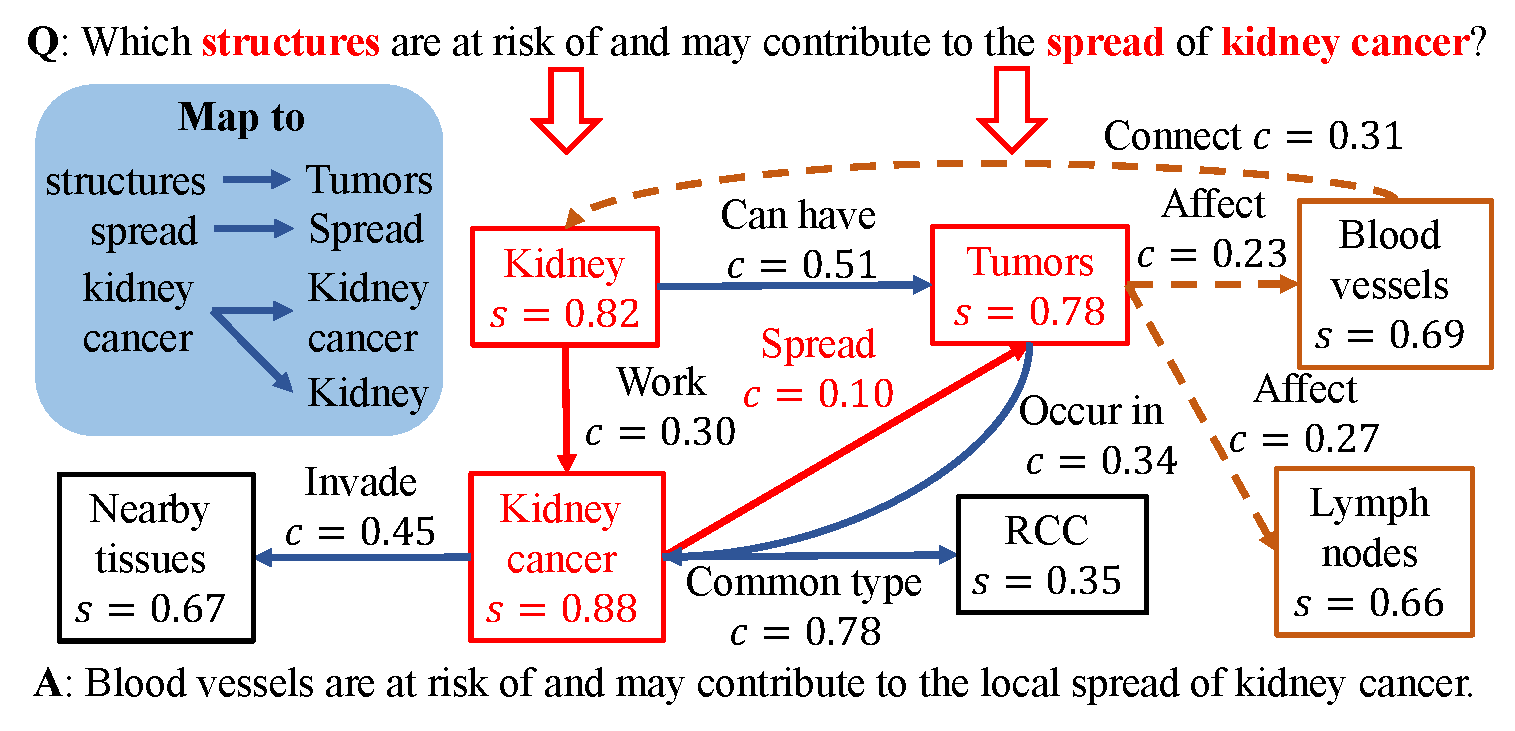
\includegraphics[width=0.88\textwidth]{figures/agrag/GERAG_example.pdf}
\caption{The original AGRAG evidence-expansion example. Red triples are query-mapped facts; orange triples show additional neighboring evidence in the illustrated MCMI structure. Reproduced from Figure 2 of the source paper~\cite{agrag-paper}.}
\label{fig:agrag:example}
\end{figure}

\subsection{The original connected-evidence example}
The running example in Figure~\ref{fig:agrag:example} makes the difference between connecting anchors and collecting an answer visible. Its mapped triples include \emph{(Kidney, Work, Kidney cancer)} and \emph{(Kidney, Spread, Tumors)}, using the relation strings printed in the original illustration. Those triples locate the query's subject region. The expanded structure additionally contains relations involving blood vessels, neighboring tissues, and other entities shown in the graph. The original illustrated answer identifies blood vessels as the requested component.

The example gives a concrete reason to inspect the neighborhood of an initial connection. The mapped facts need not name every component required in the answer. An additional relation can identify a candidate answer and connect it to the query anchors. The edge-cost and influence quantities determine how this information is considered by the expansion procedure. The selected subgraph then exposes the retained relationships to the generator as named facts, alongside its passage context.

The theoretical claims have distinct scopes. The main paper reports NP-hardness for the stated subgraph optimization problem and a 2-approximation result for the initial terminal-connecting stage. The expansion procedure adds further evidence after that stage. Its empirical contribution is evaluated by replacing the expanded subgraph with the initial Steiner-tree representation. The chapter uses this ablation to assess the role of expansion in the evaluated tasks.
% Editorial record: the supplementary monotonic-decrease argument conflicts with the sum objective; see planning/verification-agrag.md. Do not promote it to a new theorem.

The graph returned by retrieval is serialized as $g=\operatorname{StrConcat}(\mathcal{V}_{\mathrm{MCMI}},\mathcal{E}_{\mathrm{MCMI}})$. This representation contains the selected entities and relations. It makes the selected relationships available within the model's input sequence. 

\section{Hybrid Retrieval and Generation}
\label{sec:agrag:hybrid}
A graph index captures extracted relationships, whereas many details remain in the original text. AGRAG therefore also retrieves chunks through a hybrid score,
\begin{equation}
\operatorname{HS}(q,t)=\frac{\operatorname{MS}(\mathbf{q},\mathbf{t})+
\operatorname{BM25}(q,t)}{2},
\label{eq:agrag:hybrid}
\end{equation}
where $\mathbf{t}$ is the dense representation of chunk $t$. The top $k_r$ chunks according to this score form $\mathcal{T}_{\mathrm{HR}}$. The source reports $k_r=5$ in the main setting.

The two components of the score respond to different kinds of correspondence. Dense similarity compares distributed representations of a query and passage. BM25 responds to lexical overlap and term weighting~\cite{agrag-robertson2009probabilistic}. AGRAG averages the two scores as specified in the paper, then combines the selected chunks with the graph serialization. The hybrid channel is therefore an additional source of passage context rather than a separate graph expansion rule.

The final answer is generated through
\begin{equation}
A_q=\operatorname{LLM}(q,g,\mathcal{T}_{\mathrm{HR}},p_{\mathrm{gen}}).
\label{eq:agrag:generation}
\end{equation}
This input has a query, an explicit selected relational structure, and supporting passage content. The graph identifies connected facts. The passage channel supplies contextual language that graph extraction may omit. The ablations test both a graph-only condition and a hybrid-only condition, allowing the evaluation to distinguish their contributions.

For classification, the retrieval interface is adapted to return candidate labels associated with passages. One training passage per label supplies the indexed corpus. The generator selects a label from the retrieved candidate set. This setting shares the evidence-selection principle with the QA tasks, but its output and accuracy calculation are different. It is also distinct from GORAG's round-based online indexing protocol, which is examined in Chapter~\ref{ch:gorag}.

\section{Computational Properties}
\label{sec:agrag:complexity}
AGRAG's work is distributed across corpus indexing and query processing. Statistical extraction and passage-link construction operate over the corpus. Query processing includes triple mapping, filtering, graph propagation, subgraph selection, hybrid retrieval, and generation. Language-model calls contribute to relation extraction during indexing and to filtering and answer generation online.

The source's graph-operation analysis assigns $O(|\mathcal{V}||\mathcal{T}_c|)$ time to entity extraction and passage association. Graph propagation is expressed in terms of node and edge counts, and semantic edge weighting visits the indexed edges. The Mehlhorn-based initial tree stage~\cite{agrag-mehlhorn1988faster} is reported with $O(|\mathcal{E}|+|\mathcal{V}|\log|\mathcal{V}|)$ complexity. Expansion additionally depends on the selected subgraph and its neighborhood. These expressions characterize graph operations; the measured end-to-end results include model inference under the experimental configuration.

The distinction between indexing and querying is useful in deployment. An index is prepared once for a fixed corpus, while query filtering and generation recur for each query. An application with many queries can amortize index preparation, but its response latency still depends on online graph processing and the amount of generated text. Token counts and separate indexing/querying times are therefore retained in the evaluation.

The evidence graph also requires storage for entity strings, relations, and passage associations. The source gives storage in terms of graph nodes, edges, and text chunks. These objects contribute to the index storage. Practical storage depends on how embeddings, text, and adjacency structures are represented, while the experimental efficiency table reports time and token use rather than a measured memory comparison.

\section{Experimental Evaluation}
\label{sec:agrag:experiments}
\subsection{Tasks, corpora, and model settings}
The main experiment uses Novel and Medical from GraphRAG-bench~\cite{agrag-xiang2025use}, together with WOS~\cite{agrag-kowsari2017hdltex} and IFS-Rel~\cite{agrag-xia-etal-2021-incremental} for classification. Novel contains 5,140 chunks, 63,887 graph entities, and 163,169 graph relations. Medical contains 1,030 chunks, 12,426 entities, and 52,054 relations. The reported classification indexes contain 24 chunks for WOS and 11 for IFS-Rel, with 9,396 and 2,560 evaluated texts and 133 and 64 labels, respectively. These statistics are retained as reported in the source dataset table.

The Novel evaluation contains 67 creative-generation queries, 362 contextual-summarization queries, 610 complex-reasoning queries, and 971 fact-retrieval queries. The corresponding Medical counts are 166, 289, 509, and 1,098. Their differing sizes and answer requirements are relevant to interpretation. The chapter compares methods within each reported task and corpus rather than treating these query collections as interchangeable observations.

The main backbone is Qwen2.5-14B-Instruct~\cite{agrag-qwen2025qwen25technicalreport}, deployed through vLLM~\cite{agrag-kwon2023efficient}. The machine has an Intel Xeon Gold 5220R CPU and one NVIDIA A100 GPU with 80 GB memory. Contriever~\cite{agrag-izacardunsupervised} supplies dense representations for AGRAG and HippoRAG2; the other baselines use bge-large-en-v1.5 according to the reported configuration. Qwen3-Reranker-0.6B performs raw-triplet filtering. The retrieval top-$k$ setting is 5; AGRAG's raw mapped triple count and hybrid chunk count are also 5.

GraphRAG uses local search. LightRAG uses hybrid search for the QA tasks, with its classification-specific configuration retained where applicable. The comparison includes NaiveRAG, LongLLMLingua~\cite{agrag-jiang-etal-2024-longllmlingua}, RAPTOR~\cite{agrag-sarthi2024raptor}, SiReRAG~\cite{agrag-zhang2025sirerag}, G-Retriever~\cite{agrag-he2024g}, MIXRAG~\cite{agrag-liu2025mixrag}, GraphRAG~\cite{agrag-edge2024local}, LightRAG~\cite{agrag-guo2024lightrag}, HippoRAG2~\cite{agrag-gutiérrez2025ragmemory}, and Fast-GraphRAG~\cite{agrag-fastgraphrag}. These methods represent passage retrieval, compression, hierarchical organization, connected subgraph selection, neighborhood retrieval, and graph propagation. The source experiments compare their complete configurations under the stated model settings.

\subsection{Metric interpretation}
Classification accuracy is the proportion of predicted labels matching gold labels. Classification recall is macro recall. For the other tasks, the reported accuracy is a model-assessed score with values 0, 0.5, or 1 for inaccurate, partially accurate, or accurate answers. These quantities appear under the same ACC heading in the paper but evaluate different outputs.

Complex reasoning and fact retrieval additionally report the source's ROUGE-L measure~\cite{agrag-lin2004rouge}. Contextual summarization and creative generation report coverage, the fraction of required reference evidence represented in the answer. Creative generation also reports faithfulness, the fraction of answer claims supported by retrieved context. The evaluation uses the RAGAS framework~\cite{agrag-ragas2024,mgrag-es2024ragas} and the task-specific protocol. Coverage concerns inclusion of required information, whereas faithfulness concerns support for generated claims.

For generated answer sequence $G$ and reference sequence $Y$, the source defines its reported lexical score as
\begin{equation}
\operatorname{ROG}(G,Y)=\frac{\operatorname{LCS}(G,Y)}{|G|}.
\label{eq:agrag:rouge}
\end{equation}
The denominator is the generated answer length. This is the source's reported ROUGE-L quantity, rather than an F1 combination of longest-common-subsequence precision and recall. Retaining the denominator is necessary when interpreting a short factual answer alongside a longer response.

Let $E$ denote the reference evidence items and let $M(e,R)$ indicate whether response $R$ covers item $e$. Coverage is
\begin{equation}
\operatorname{COV}(R,E)=\frac{|\{e\in E:M(e,R)\}|}{|E|}.
\label{eq:agrag:coverage}
\end{equation}
For the answer's claim set $A$ and retrieved context $C$, let $S(a,C)$ indicate that claim $a$ is supported. Faithfulness is
\begin{equation}
\operatorname{FS}(A,C)=\frac{|\{a\in A:S(a,C)\}|}{|A|}.
\label{eq:agrag:faithfulness}
\end{equation}
The two denominators identify different evidence requirements. Coverage uses the required reference information; faithfulness uses the claims actually made. A response omitting a required fact can lose coverage even when its remaining statements are supported. Conversely, adding unsupported claims affects faithfulness even if all reference evidence is mentioned. The source evaluates these judgments through its model-based assessment procedure. The measures therefore retain the evaluator and evidence units of that protocol.

\begin{table}[tbp]
\centering\small
\setlength{\tabcolsep}{3pt}
\caption{Creative generation with Qwen2.5-14B-Instruct. Results from the AGRAG main experiment~\cite{agrag-paper}.}
\label{tab:agrag:main-creative}
\resizebox{\textwidth}{!}{%
\begin{tabular}{lrrrrrr}
\toprule
Method & Novel FS & Novel ACC & Novel COV & Medical FS & Medical ACC & Medical COV\\
\midrule
NaiveRAG & 0.205 & 0.307 & \underline{0.384} & 0.176 & \underline{0.577} & \underline{0.554}\\
L.LLMLingua & 0.213 & 0.316 & 0.377 & 0.225 & 0.575 & 0.496\\
RAPTOR & 0.365 & \underline{0.333} & 0.373 & 0.314 & 0.526 & 0.553\\
SiReRAG & 0.324 & 0.328 & 0.365 & 0.295 & 0.544 & 0.456\\
G-retriever & 0.294 & 0.167 & 0.200 & 0.169 & 0.371 & 0.468\\
MIXRAG & 0.200 & 0.286 & 0.337 & 0.255 & 0.351 & 0.306\\
GraphRAG & 0.427 & 0.310 & 0.339 & 0.345 & 0.475 & 0.325\\
LightRAG & 0.201 & 0.314 & 0.329 & 0.189 & 0.567 & 0.549\\
HippoRAG2 & \underline{0.496} & 0.295 & 0.325 & \underline{0.347} & 0.563 & 0.451\\
F.GraphRAG & 0.286 & 0.287 & 0.376 & 0.217 & 0.500 & 0.396\\
\textbf{AGRAG} & \textbf{0.513} & \textbf{0.339} & \textbf{0.386} & \textbf{0.356} & \textbf{0.598} & \textbf{0.589}\\
\bottomrule
\end{tabular}}
\end{table}

\begin{table}[tbp]
\centering\small
\setlength{\tabcolsep}{3pt}
\caption{Contextual summarization with Qwen2.5-14B-Instruct. Results from the AGRAG main experiment~\cite{agrag-paper}.}
\label{tab:agrag:main-summary}
\resizebox{\textwidth}{!}{%
\begin{tabular}{lrrrr}
\toprule
Method & Novel COV & Novel ACC & Medical COV & Medical ACC\\
\midrule
NaiveRAG & 0.745 & 0.621 & \underline{0.677} & 0.576\\
L.LLMLingua & 0.687 & 0.627 & 0.657 & 0.583\\
RAPTOR & \underline{0.760} & 0.626 & 0.633 & 0.583\\
SiReRAG & 0.754 & 0.617 & 0.592 & 0.560\\
G-retriever & 0.594 & 0.404 & 0.302 & 0.395\\
MIXRAG & 0.695 & 0.538 & 0.409 & 0.464\\
GraphRAG & 0.758 & 0.620 & 0.625 & 0.506\\
LightRAG & 0.753 & \underline{0.628} & 0.625 & 0.585\\
HippoRAG2 & 0.735 & 0.586 & 0.496 & 0.560\\
F.GraphRAG & 0.706 & 0.528 & 0.507 & \underline{0.587}\\
\textbf{AGRAG} & \textbf{0.778} & \textbf{0.643} & \textbf{0.690} & \textbf{0.604}\\
\bottomrule
\end{tabular}}
\end{table}

\begin{table}[tbp]
\centering\small
\setlength{\tabcolsep}{3pt}
\caption{Complex reasoning with Qwen2.5-14B-Instruct. Results from the AGRAG main experiment~\cite{agrag-paper}.}
\label{tab:agrag:main-complex}
\resizebox{\textwidth}{!}{%
\begin{tabular}{lrrrr}
\toprule
Method & Novel ROG & Novel ACC & Medical ROG & Medical ACC\\
\midrule
NaiveRAG & 0.120 & 0.447 & 0.117 & 0.635\\
L.LLMLingua & 0.092 & 0.434 & 0.080 & 0.633\\
RAPTOR & 0.290 & \underline{0.460} & 0.185 & \underline{0.649}\\
SiReRAG & 0.307 & 0.459 & 0.269 & 0.646\\
G-retriever & 0.146 & 0.441 & 0.102 & 0.396\\
MIXRAG & 0.109 & 0.386 & 0.156 & 0.434\\
GraphRAG & 0.246 & 0.449 & 0.250 & 0.606\\
LightRAG & 0.223 & 0.448 & 0.255 & 0.637\\
HippoRAG2 & \underline{0.314} & 0.453 & \underline{0.332} & 0.622\\
F.GraphRAG & 0.237 & 0.371 & 0.262 & 0.643\\
\textbf{AGRAG} & \textbf{0.319} & \textbf{0.467} & \textbf{0.343} & \textbf{0.665}\\
\bottomrule
\end{tabular}}
\end{table}

\begin{table}[tbp]
\centering\small
\setlength{\tabcolsep}{3pt}
\caption{Fact retrieval with Qwen2.5-14B-Instruct. Results from the AGRAG main experiment~\cite{agrag-paper}.}
\label{tab:agrag:main-fact}
\resizebox{\textwidth}{!}{%
\begin{tabular}{lrrrr}
\toprule
Method & Novel ROG & Novel ACC & Medical ROG & Medical ACC\\
\midrule
NaiveRAG & 0.117 & 0.431 & 0.182 & 0.604\\
L.LLMLingua & 0.115 & 0.420 & 0.105 & 0.591\\
RAPTOR & 0.133 & 0.465 & 0.132 & 0.609\\
SiReRAG & 0.311 & 0.451 & 0.349 & 0.558\\
G-retriever & 0.199 & 0.209 & 0.148 & 0.326\\
MIXRAG & 0.102 & 0.366 & 0.160 & 0.463\\
GraphRAG & 0.240 & 0.445 & 0.217 & 0.521\\
LightRAG & 0.253 & 0.460 & 0.283 & 0.607\\
HippoRAG2 & 0.310 & \underline{0.470} & 0.343 & 0.598\\
F.GraphRAG & \underline{0.318} & 0.439 & \underline{0.352} & \underline{0.610}\\
\textbf{AGRAG} & \textbf{0.324} & \textbf{0.490} & \textbf{0.357} & \textbf{0.628}\\
\bottomrule
\end{tabular}}
\end{table}

\begin{table}[tbp]
\centering\small
\setlength{\tabcolsep}{3pt}
\caption{Text classification with Qwen2.5-14B-Instruct. Results from the AGRAG main experiment~\cite{agrag-paper}.}
\label{tab:agrag:main-class}
\resizebox{\textwidth}{!}{%
\begin{tabular}{lrrrr}
\toprule
Method & WOS ACC & WOS REC & IFS-Rel ACC & IFS-Rel REC\\
\midrule
NaiveRAG & 0.237 & 0.257 & 0.351 & 0.197\\
L.LLMLingua & 0.274 & 0.231 & 0.378 & 0.220\\
RAPTOR & 0.409 & 0.290 & 0.293 & 0.212\\
SiReRAG & \underline{0.430} & \underline{0.294} & 0.325 & 0.220\\
G-retriever & 0.188 & 0.129 & 0.311 & 0.185\\
MIXRAG & 0.244 & 0.235 & 0.362 & 0.203\\
GraphRAG & 0.253 & 0.201 & 0.279 & 0.202\\
LightRAG & 0.273 & 0.224 & 0.265 & 0.220\\
HippoRAG2 & 0.424 & 0.270 & \underline{0.389} & \underline{0.246}\\
F.GraphRAG & 0.283 & 0.245 & 0.307 & 0.221\\
\textbf{AGRAG} & \textbf{0.438} & \textbf{0.307} & \textbf{0.403} & \textbf{0.251}\\
\bottomrule
\end{tabular}}
\end{table}


\subsection{Answer quality across tasks}
The main results are split by task in Tables~\ref{tab:agrag:main-creative}--\ref{tab:agrag:main-class}. On Novel creative generation, AGRAG reports faithfulness 0.513, accuracy 0.339, and coverage 0.386. HippoRAG2 reports faithfulness 0.496, while RAPTOR reports accuracy 0.333 and NaiveRAG coverage 0.384. The close coverage values and the different best comparison methods show why one baseline cannot summarize every metric.

On Medical creative generation, AGRAG reports faithfulness 0.356, accuracy 0.598, and coverage 0.589. NaiveRAG has accuracy 0.577 and coverage 0.554. HippoRAG2 has faithfulness 0.347. The task combines contextual grounding with a more flexible response format, and the three measures capture different aspects of that response.

For contextual summarization, AGRAG obtains coverage and accuracy of 0.778 and 0.643 on Novel, and 0.690 and 0.604 on Medical. The task requires collecting information distributed across the evidence. The result is consistent with the design of supplying connected graph facts together with passage context. The ablations provide the more direct component comparison by removing either the graph structure or the hybrid channel.

For complex reasoning, the reported ROUGE-L and accuracy values are 0.319 and 0.467 on Novel and 0.343 and 0.665 on Medical. For fact retrieval they are 0.324 and 0.490 on Novel and 0.357 and 0.628 on Medical. The tasks use different query collections and answer formats.

Classification accuracy and recall are 0.438 and 0.307 on WOS and 0.403 and 0.251 on IFS-Rel. SiReRAG reports WOS accuracy 0.430 and recall 0.294, while HippoRAG2 reports IFS-Rel accuracy 0.389 and recall 0.246. AGRAG's classifier receives graph-derived candidate labels under the source protocol. The results evaluate the combined retrieval and label-selection pipeline, so improvements cannot be assigned solely to the final language-model decision.

\subsection{Indexing and querying costs}
\begin{table}[tbp]
\centering\small
\setlength{\tabcolsep}{3pt}
\caption{Indexing / querying time in minutes. Qwen2.5-14B-Instruct; original paired measurements are preserved.}
\label{tab:agrag:efficiency}
\resizebox{\textwidth}{!}{%
\begin{tabular}{lrrrr}
\toprule
Method & Novel & Medical & WOS & IFS-Rel\\
\midrule
NaiveRAG & 13 / 371 & 7 / 245 & 2 / 292 & 2 / 225\\
L.LLMLingua & 51 / 360 & 37 / 305 & 4 / 358 & 3 / 315\\
RAPTOR & 464 / 250 & 117 / 319 & 30 / 162 & 24 / 121\\
SiReRAG & 85 / 233 & 40 / 207 & 26 / 139 & 18 / 117\\
G-Retriever & 19 / 119 & 12 / 145 & 8 / 158 & 3 / 164\\
MIXRAG & 17 / 388 & 11 / 453 & 5 /  257 & 2 / 193\\
GraphRAG & 347 / 205 & 194 / 158 & 85 / 240 & 64 / 217\\
LightRAG & 166 / 221 & 116 / 164 & 42 / 211 & 31 / 197\\
HippoRAG2 & 95 / 134 & 46 / 130 & 19 / 140 & 15 / 127\\
F.GraphRAG & 106 / 198 & 48 / 173 & 29 / 186 & 27 / 164\\
\textbf{AGRAG} & 65 / 142 & 16 / 138 & 16 / 132 & 14 / 124\\
\bottomrule
\end{tabular}}
\end{table}
\begin{table}[tbp]
\centering\small
\setlength{\tabcolsep}{3pt}
\caption{Input / output tokens per query. Same source experiment as the preceding time table.}
\label{tab:agrag:efficiency-tokens}
\resizebox{\textwidth}{!}{%
\begin{tabular}{lrrrr}
\toprule
Method & Novel & Medical & WOS & IFS-Rel\\
\midrule
NaiveRAG & 9,437 / 1,708 & 7,473 / 379 & 7,292 / 29 & 4,521 / 16\\
L.LLMLingua & 8,466 / 1,750 & 5,686 / 390 & 5,861 / 31 & 2,757 / 14\\
RAPTOR & 7,243 / 777 & 4,817 / 695 & 6,007 / 41 & 3,807 / 33\\
SiReRAG & 7,759 / 800 & 4,918 / 701 & 6,012 / 47 & 3,821 / 36\\
G-Retriever & 6,344 / 116 & 6,290 / 157 & 6,762 / 12 & 4,002 / 21\\
MIXRAG & 6,083 / 237 & 4,238 / 230 & 4,193 / 31 & 3,597 / 29\\
GraphRAG & 12,686 / 2,109 & 8,385 / 1,017 & 11,809 / 351 & 9,009 / 287\\
LightRAG & 13,145 / 1,233 & 9,535 / 426 & 11,510 / 227 & 7,667 / 199\\
HippoRAG2 & 8,138 / 1,073 & 6,264 / 595 & 5,066 / 93 & 2,440 / 102\\
F.GraphRAG & 7,490 / 1,252 & 6,475 / 384 & 4,957 / 35 & 2,217 / 20\\
\textbf{AGRAG} & 6,487 / 1,140 & 5,145 / 413 & 3,970 / 101 & 1,890 / 93\\
\bottomrule
\end{tabular}}
\end{table}

Table~\ref{tab:agrag:efficiency} separates indexing time, querying time, input tokens, and output tokens. For Novel, AGRAG reports 65 minutes for indexing and 142 minutes for querying, compared with HippoRAG2's 95 and 134 minutes. For Medical the corresponding values are 16 and 138 minutes for AGRAG and 46 and 130 minutes for HippoRAG2. This comparison shows lower index preparation time alongside a higher reported query total for AGRAG.

The table also contains methods with lower costs in particular columns. NaiveRAG has lower indexing times, while G-Retriever has a shorter Novel querying total. 

On WOS and IFS-Rel, AGRAG reports querying times of 132 and 124 minutes and input token counts of 3,970 and 1,890 per query. The corresponding HippoRAG2 values are 140 and 127 minutes and 5,066 and 2,440 tokens. Output lengths differ between methods. Preserving both input and output counts helps distinguish the amount of supplied evidence from the cost of producing an answer.

\subsection{Component ablations}
\begin{table}[tbp]
\centering\small
\setlength{\tabcolsep}{3pt}
\caption{Creative generation ablation with Qwen2.5-14B-Instruct. Values retain the original source ablation precision.}
\label{tab:agrag:ablation}
\resizebox{\textwidth}{!}{%
\begin{tabular}{lrrrrrr}
\toprule
Method & Novel FS & Novel ACC & Novel COV & Medical FS & Medical ACC & Medical COV\\
\midrule
AGRAG w. HR Only & 0.491 & 0.322 & 0.378 & 0.303 & 0.526 & 0.549\\
AGRAG w. LLM ER & 0.428 & 0.302 & 0.365 & 0.352 & 0.526 & 0.587\\
AGRAG w.o. HR & 0.519 & 0.306 & 0.343 & 0.342 & 0.521 & 0.570\\
AGRAG w.o. MCMI & 0.488 & 0.332 & 0.358 & 0.351 & 0.530 & 0.575\\
AGRAG w.o. Cle. & 0.478 & 0.311 & 0.361 & 0.336 & 0.517 & 0.569\\
\textbf{AGRAG} & 0.513 & 0.339 & 0.386 & 0.356 & 0.598 & 0.589\\
\bottomrule
\end{tabular}}
\end{table}
\begin{table}[tbp]
\centering\small
\setlength{\tabcolsep}{3pt}
\caption{Contextual summarization ablation with Qwen2.5-14B-Instruct. Values retain the original source ablation precision.}
\label{tab:agrag:ablation-summary}
\resizebox{\textwidth}{!}{%
\begin{tabular}{lrrrr}
\toprule
Method & Novel COV & Novel ACC & Medical COV & Medical ACC\\
\midrule
AGRAG w. HR Only & 0.739 & 0.522 & 0.535 & 0.583\\
AGRAG w. LLM ER & 0.755 & 0.552 & 0.600 & 0.566\\
AGRAG w.o. HR & 0.677 & 0.534 & 0.420 & 0.578\\
AGRAG w.o. MCMI & 0.748 & 0.592 & 0.600 & 0.588\\
AGRAG w.o. Cle. & 0.712 & 0.597 & 0.616 & 0.577\\
\textbf{AGRAG} & 0.778 & 0.643 & 0.690 & 0.604\\
\bottomrule
\end{tabular}}
\end{table}
\begin{table}[tbp]
\centering\small
\setlength{\tabcolsep}{3pt}
\caption{Complex reasoning ablation with Qwen2.5-14B-Instruct. Values retain the original source ablation precision.}
\label{tab:agrag:ablation-complex}
\resizebox{\textwidth}{!}{%
\begin{tabular}{lrrrr}
\toprule
Method & Novel ROG & Novel ACC & Medical ROG & Medical ACC\\
\midrule
AGRAG w. HR Only & 0.303 & 0.453 & 0.334 & 0.636\\
AGRAG w. LLM ER & 0.320 & 0.465 & 0.333 & 0.624\\
AGRAG w.o. HR & 0.318 & 0.434 & 0.324 & 0.598\\
AGRAG w.o. MCMI & 0.324 & 0.465 & 0.329 & 0.633\\
AGRAG w.o. Cle. & 0.301 & 0.450 & 0.334 & 0.628\\
\textbf{AGRAG} & 0.319 & 0.467 & 0.343 & 0.665\\
\bottomrule
\end{tabular}}
\end{table}
\begin{table}[tbp]
\centering\small
\setlength{\tabcolsep}{3pt}
\caption{Fact retrieval ablation with Qwen2.5-14B-Instruct. Values retain the original source ablation precision.}
\label{tab:agrag:ablation-fact}
\resizebox{\textwidth}{!}{%
\begin{tabular}{lrrrr}
\toprule
Method & Novel ROG & Novel ACC & Medical ROG & Medical ACC\\
\midrule
AGRAG w. HR Only & 0.323 & 0.487 & 0.355 & 0.619\\
AGRAG w. LLM ER & 0.322 & 0.480 & 0.353 & 0.613\\
AGRAG w.o. HR & 0.314 & 0.487 & 0.344 & 0.615\\
AGRAG w.o. MCMI & 0.322 & 0.470 & 0.359 & 0.621\\
AGRAG w.o. Cle. & 0.313 & 0.478 & 0.354 & 0.620\\
\textbf{AGRAG} & 0.324 & 0.490 & 0.357 & 0.628\\
\bottomrule
\end{tabular}}
\end{table}
\begin{table}[tbp]
\centering\small
\setlength{\tabcolsep}{3pt}
\caption{Ablation time and token costs. Time is in minutes. Paired token columns retain the source I/G headings; its caption describes input/output token counts.}
\label{tab:agrag:ablation-cost}
\resizebox{\textwidth}{!}{%
\begin{tabular}{lrrrr}
\toprule
Method & Novel time I/Q & Novel tokens I/G & Medical time I/Q & Medical tokens I/G\\
\midrule
AGRAG w. HR Only & 11.7 / 137.9 & 5,117 / 193 & 11.4 / 117.9 & 5,215 / 199\\
AGRAG w. LLM ER & 83.3 /  161.2 & 8,030 /   887 & 31.9 / 148.8 & 5,457  / 414\\
AGRAG w.o. HR & 61.7 / 138.9 & 6,986 / 741 & 9.4 / 114.4 & 4,820 / 315\\
AGRAG w.o. MCMI & 63.9 / 130.4 & 6,710 / 757 & 9.5 /  125.0 & 5,230 /    331\\
AGRAG w.o. Cle. & 65.6 / 140.1 & 6,988 / 154 & 9.1 / 142.9 & 5,252 / 158\\
\textbf{AGRAG} & 65.6 / 142.0 & 6,988 / 639 & 9.1 / 145.3 & 5,252 / 306\\
\bottomrule
\end{tabular}}
\end{table}

The ablation compares hybrid retrieval alone, language-model entity extraction, graph retrieval without hybrid context, an initial tree without MCMI expansion, and retrieval without the raw-triplet filtering step. These interventions act on different parts of the pipeline. They therefore give more specific evidence than the comparison between complete systems.

The hybrid-only variant has Novel creative-generation faithfulness 0.491, accuracy 0.322, and coverage 0.378. Full AGRAG reports 0.513, 0.339, and 0.386. For Novel contextual summarization, hybrid-only coverage and accuracy are 0.739 and 0.522, compared with 0.778 and 0.643 for the complete system. The graph-containing configuration provides an observed benefit under these settings, particularly for the summarization accuracy score.

Removing hybrid retrieval produces a different pattern. Novel creative-generation faithfulness is 0.519, exceeding the complete system's 0.513, while accuracy and coverage decrease to 0.306 and 0.343. Medical contextual-summarization coverage decreases from 0.690 to 0.420. The graph-only variant can produce well-grounded claims while supplying less of the required information.

Replacing statistical entity extraction with model-based extraction gives Novel creative-generation faithfulness 0.428 and accuracy 0.302, with indexing time 83.3 minutes in the ablation setting. The complete configuration reports 65.6 minutes in that table. This experiment changes entity extraction while retaining the rest of the method.

The variant without MCMI expansion uses a Steiner-tree representation. Its Novel contextual-summarization accuracy is 0.592, compared with 0.643 for full AGRAG, and its Medical creative-generation accuracy is 0.530, compared with 0.598. Some fact-retrieval metrics are close or favor the tree variant. Expansion is thus most informative in the evaluated tasks that require gathering and combining additional evidence, while the table preserves cases where the simpler representation performs similarly.

Removing raw-triplet filtering gives Novel contextual-summarization coverage 0.712 and accuracy 0.597. These are below 0.778 and 0.643 for full AGRAG. The ablation evaluates whether the initial semantic mapping alone supplies appropriate query anchors. Its results support retaining the filtering stage under the reported configuration.

The ablation and main efficiency tables use separate reported measurements. For example, the Medical indexing/querying totals differ between the tables. Both sets of values are retained in their original experimental contexts. They are not averaged or substituted for one another when discussing a component intervention.

\subsection{Additional resource setting and parameter study}
\begin{table}[tbp]
\centering\small
\setlength{\tabcolsep}{3pt}
\caption{Creative generation in the low-resource setting. Qwen3-4B-Instruct-2507 on two 2080 Ti GPUs; values and emphasis preserved.}
\label{tab:agrag:low-resource}
\resizebox{\textwidth}{!}{%
\begin{tabular}{lrrrrrr}
\toprule
Method & Novel FS & Novel ACC & Novel COV & Medical FS & Medical ACC & Medical COV\\
\midrule
SiReRAG-L & 0.324 & 0.412 & 0.299 & 0.421 & \underline{0.758} & \underline{0.475}\\
HippoRAG2-L & \underline{0.433} & \underline{0.481} & \underline{0.335} & \underline{0.425} & 0.755 & 0.433\\
\textbf{AGRAG-L} & \textbf{0.441} & \textbf{0.519} & \textbf{0.354} & \textbf{0.436} & \textbf{0.777} & \textbf{0.490}\\
\bottomrule
\end{tabular}}
\end{table}
\begin{table}[tbp]
\centering\small
\setlength{\tabcolsep}{3pt}
\caption{Contextual summarization in the low-resource setting. Qwen3-4B-Instruct-2507 on two 2080 Ti GPUs; values and emphasis preserved.}
\label{tab:agrag:low-resource-summary}
\resizebox{\textwidth}{!}{%
\begin{tabular}{lrrrr}
\toprule
Method & Novel COV & Novel ACC & Medical COV & Medical ACC\\
\midrule
SiReRAG-L & 0.647 & \underline{0.673} & \underline{0.536} & \underline{0.738}\\
HippoRAG2-L & \underline{0.696} & 0.657 & 0.522 & 0.731\\
\textbf{AGRAG-L} & \textbf{0.745} & \textbf{0.706} & \textbf{0.545} & \textbf{0.751}\\
\bottomrule
\end{tabular}}
\end{table}
\begin{table}[tbp]
\centering\small
\setlength{\tabcolsep}{3pt}
\caption{Complex reasoning in the low-resource setting. Qwen3-4B-Instruct-2507 on two 2080 Ti GPUs; values and emphasis preserved.}
\label{tab:agrag:low-resource-complex}
\resizebox{\textwidth}{!}{%
\begin{tabular}{lrrrr}
\toprule
Method & Novel ROG & Novel ACC & Medical ROG & Medical ACC\\
\midrule
SiReRAG-L & 0.260 & 0.426 & \underline{0.308} & \underline{0.698}\\
HippoRAG2-L & \underline{0.280} & \underline{0.507} & 0.298 & 0.681\\
\textbf{AGRAG-L} & \textbf{0.293} & \textbf{0.552} & \textbf{0.312} & \textbf{0.739}\\
\bottomrule
\end{tabular}}
\end{table}
\begin{table}[tbp]
\centering\small
\setlength{\tabcolsep}{3pt}
\caption{Fact retrieval in the low-resource setting. Qwen3-4B-Instruct-2507 on two 2080 Ti GPUs; values and emphasis preserved.}
\label{tab:agrag:low-resource-fact}
\resizebox{\textwidth}{!}{%
\begin{tabular}{lrrrr}
\toprule
Method & Novel ROG & Novel ACC & Medical ROG & Medical ACC\\
\midrule
SiReRAG-L & 0.271 & 0.416 & \underline{0.343} & \underline{0.661}\\
HippoRAG2-L & \underline{0.288} & \underline{0.513} & 0.338 & 0.654\\
\textbf{AGRAG-L} & \textbf{0.297} & \textbf{0.560} & \textbf{0.351} & \textbf{0.701}\\
\bottomrule
\end{tabular}}
\end{table}

\begin{table}[tbp]
\centering\small
\setlength{\tabcolsep}{3pt}
\caption{Novel low-resource efficiency. Qwen3-4B-Instruct-2507 on two 2080 Ti GPUs.}
\label{tab:agrag:low-resource-efficiency}
\resizebox{\textwidth}{!}{%
\begin{tabular}{lrrrr}
\toprule
Method & Index min & Query min & Input tokens & Output tokens\\
\midrule
SiReRAG-L & \underline{52.0} & 183.5 & \underline{7,898} & \textbf{1,003}\\
HippoRAG2-L & 55.7 & \textbf{131.2} & 7,964 & 1,354\\
\textbf{AGRAG-L} & \textbf{44.7} & \underline{132.1} & \textbf{6,625} & \underline{1,172}\\
\bottomrule
\end{tabular}}
\end{table}
\begin{table}[tbp]
\centering\small
\setlength{\tabcolsep}{3pt}
\caption{Medical low-resource efficiency. Qwen3-4B-Instruct-2507 on two 2080 Ti GPUs.}
\label{tab:agrag:low-resource-efficiency-medical}
\resizebox{\textwidth}{!}{%
\begin{tabular}{lrrrr}
\toprule
Method & Index min & Query min & Input tokens & Output tokens\\
\midrule
SiReRAG-L & 18.1 & 182.3 & \textbf{5,113} & 827\\
HippoRAG2-L & \underline{21.8} & \textbf{162.4} & 5,577 & \underline{584}\\
\textbf{AGRAG-L} & \textbf{14.4} & \underline{167.3} & \underline{5,282} & \textbf{534}\\
\bottomrule
\end{tabular}}
\end{table}

The low-resource experiment uses Qwen3-4B-Instruct-2507 on two NVIDIA 2080 Ti GPUs. This changes both model and hardware relative to the main experiment. The comparison therefore concerns the methods within that resource setting. It supplies evidence about operating with a smaller backbone and different accelerators rather than a controlled estimate of the effect of model size alone.

In that setting, AGRAG-L reports Novel creative-generation accuracy 0.519 and contextual-summarization accuracy 0.706. Its Novel index/query totals are 44.7 and 132.1 minutes. Medical totals are 14.4 and 167.3 minutes. HippoRAG2-L has shorter query totals in both corpora, while AGRAG-L has shorter indexing totals. The complete low-resource tables retain the quality and token measures needed to assess those tradeoffs.

The parameter study varies the maximum n-gram length over $\{1,3,5,7\}$ and the extraction threshold over $\{0.1,0.3,0.5,0.7\}$. The original heatmaps are reproduced in Figure~\ref{fig:agrag:sensitivity}. They show accuracy across the tested combinations for Novel and Medical. The main experiment uses $b=3$ and $\tau=0.5$. 

\begin{figure}[!htbp]
\centering
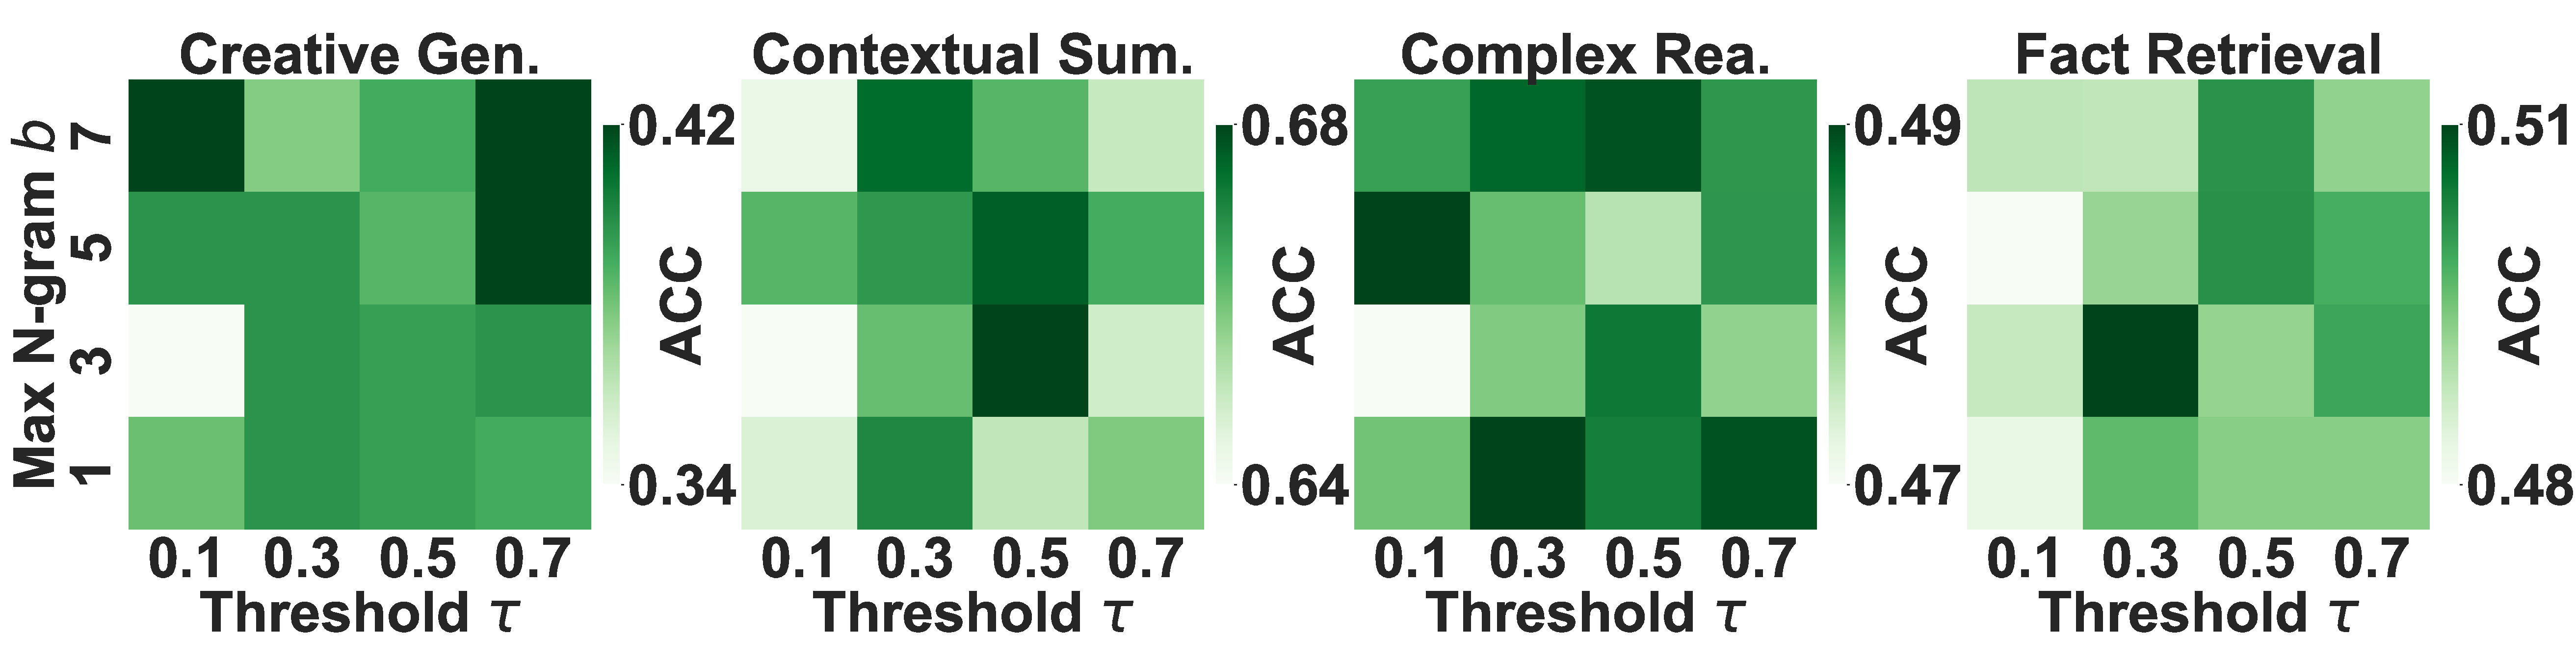
\includegraphics[width=0.95\textwidth]{figures/agrag/heatmap_novel.pdf}\\[1em]
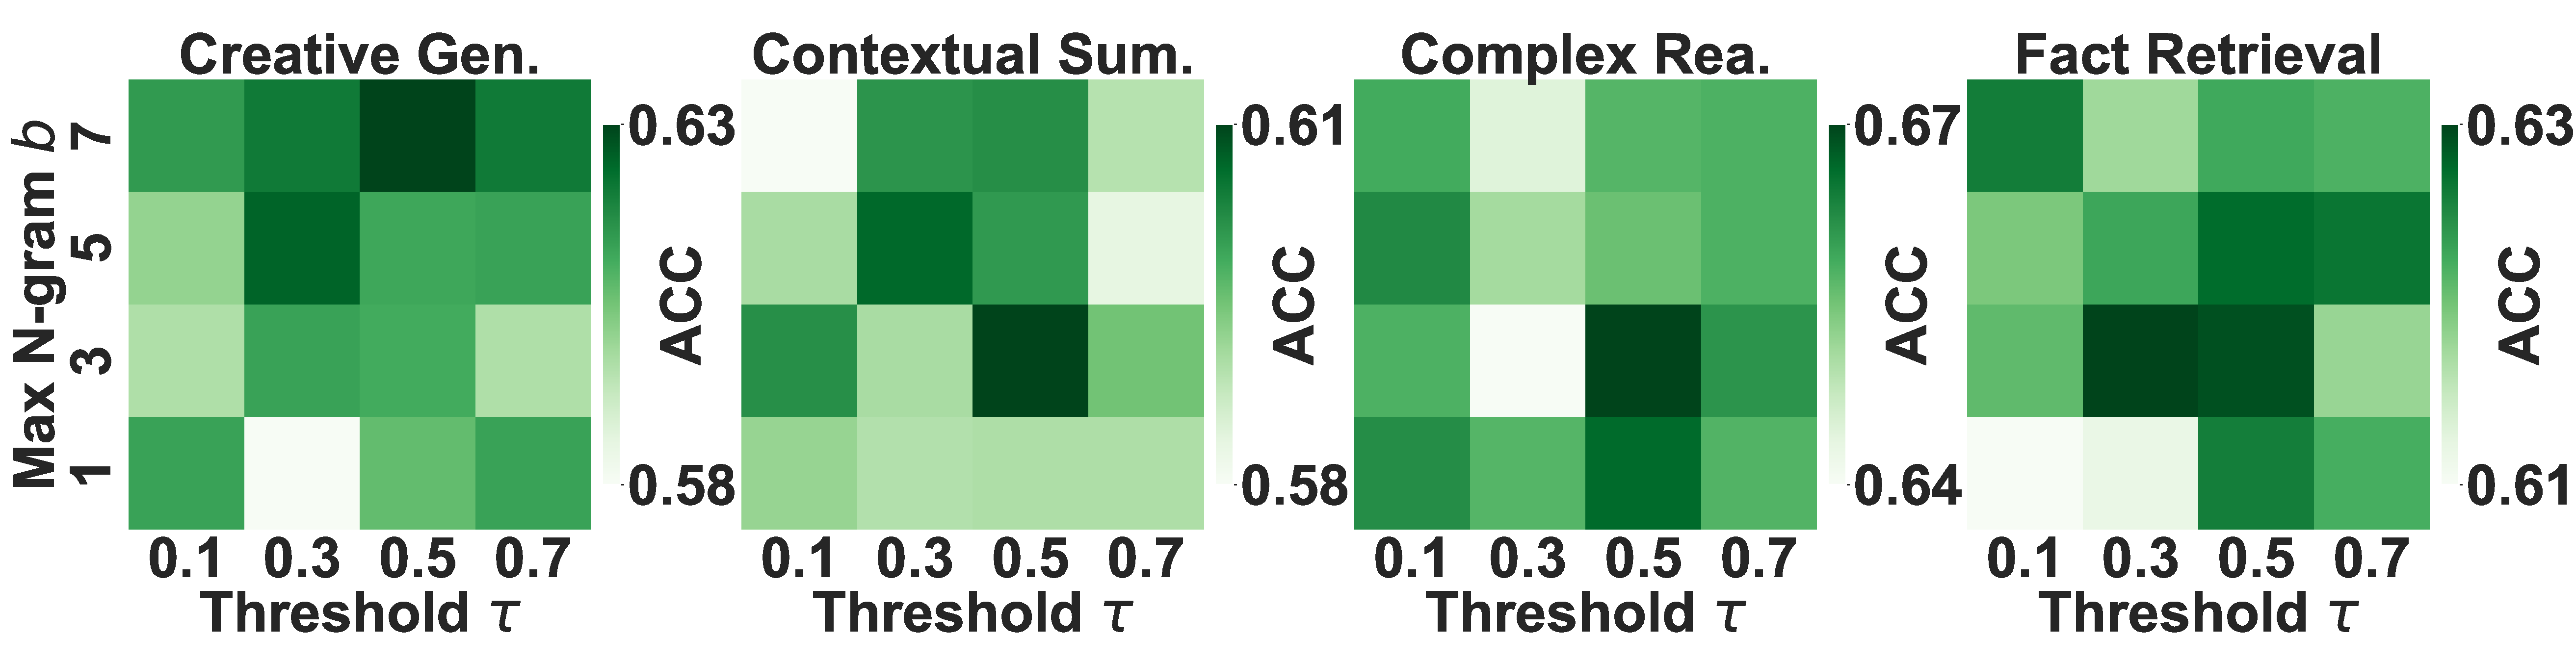
\includegraphics[width=0.95\textwidth]{figures/agrag/heatmap_medical.pdf}
\caption{AGRAG parameter sensitivity on Novel (top) and Medical (bottom). The original panels vary the extraction threshold and maximum n-gram length and display task accuracy. Reproduced from Figure 3 of the source paper~\cite{agrag-paper}.}
\label{fig:agrag:sensitivity}
\end{figure}

\section{Discussion and Chapter Summary}
\label{sec:agrag:discussion}
AGRAG places structure at two points in the evidence pipeline. Graph construction determines which entities, relations, and passage links are available. Query-time selection determines how those items are connected in the context supplied to the generator. The hybrid retriever preserves a route to passage information outside the selected graph. The method consequently treats graph evidence and textual context as complementary representations of the indexed corpus.

% Keep this discussion paragraph intact after the full-width parameter figure.
\begin{samepage}
The experimental distinction between faithfulness and coverage is especially relevant to the thesis. Removing hybrid context can retain or improve one grounding measure while decreasing the amount of required evidence expressed in an answer. Replacing the expanded subgraph with a tree affects the evaluated tasks differently. These observations relate the retrieval representation to specific answer requirements instead of treating a graph as a universal improvement over a passage list.\par
\end{samepage}

The remaining conditions concern the evidence source and the language-model interface. Relations are model-extracted, query anchors are model-filtered, and several QA metrics use model assessment. Statistical entity selection constrains entity strings to the corpus, but relation quality and evaluation remain important to the interpretation of the reported scores. A complete application must also account for corpus preparation, online retrieval, and answer generation separately.

The chapter answers the third research question by developing a pipeline that combines node influence, semantic edge costs, connected evidence selection, and hybrid passage context. The published experiments identify its effects across fact retrieval, complex reasoning, summarization, creative generation, and classification. Chapter~\ref{ch:mgrag} adds multimodal evidence and asks how a query graph can match semantically corresponding paths even when the query and evidence graphs have different topologies.

\chapter{Semantic Graph Matching for Multimodal Reasoning with MGRAG}
\label{ch:mgrag}

This chapter is based on \emph{MGRAG: Semantic Subgraph Matching and Graph-Aware Caching for Multimodal Retrieval-Augmented Generation}, published in the \emph{Proceedings of the VLDB Endowment}, volume 19, number 9, pages 2480--2493, 2026~\cite{mgrag-paper}. It studies how a query can determine the evidence graph to construct, how paths can express semantic correspondences across different graph topologies, and how the resulting structure can guide context computation.

\section{Multimodal Evidence and Query Requirements}
\label{sec:mgrag:problem}

An answer to a multimodal query may depend on a relation that is distributed across text and images. A document can name a person, an image can show an action, and another passage can connect that person to an event. Retrieving each item by its similarity to the query supplies candidate evidence, but the relation needed for the answer can remain implicit. A graph makes the entities and their connections available as a retrieval object. Its usefulness depends on which facts are extracted and on whether its representation can express the relation requested by the query.

This chapter considers a corpus $\mathcal D=\mathcal D_{\mathrm{txt}}\cup\mathcal D_{\mathrm{img}}$ and a query $q$ that can contain text, an image, or both. A retrieval module selects evidence from the corpus, and a multimodal language model generates an answer using that evidence. The research question is how to construct and retrieve a query-relevant relational representation while controlling the cost of preparing and processing the context. The answer-generation task remains grounded in the original documents and images. The graph supplies an additional representation of their query-related content.

Three decisions govern this process. The first concerns when to construct a graph. A corpus-wide graph requires extraction before the query is known. Its entities and relations consequently reflect the extraction prompt's general description of the corpus. When an image contains several people, objects, and actions, the details relevant to one query can differ from those relevant to another. MGRAG places the query inside the extraction process and constructs the graph incrementally from ranked evidence. The graph is specific to the current query.

The second decision concerns what constitutes a match. A query and its supporting documents need not use the same decomposition of a fact. The published motivating example describes a data graph containing two \texttt{father\_of} edges and a query containing one \texttt{grandfather\_of} edge. The requested relation is represented by a two-hop path in the data. Requiring the same edge topology would exclude this correspondence. Figure~\ref{fig:mgrag:motivation} reproduces the example. MGRAG evaluates semantic representations of paths so that a query relation can be supported by a sequence of evidence relations.

\begin{figure}[tbp]
\centering
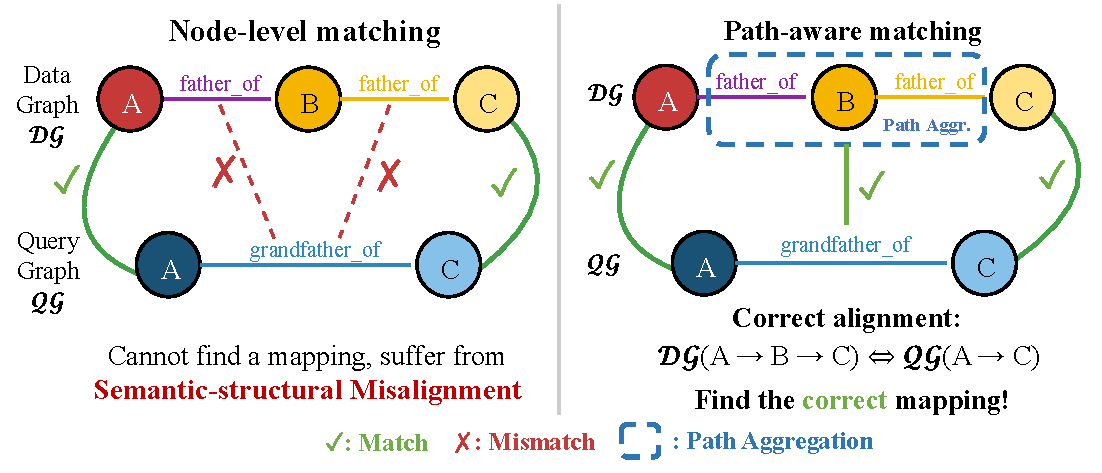
\includegraphics[width=0.85\textwidth]{figures/mgrag/motivation.pdf}
\caption{Path-level correspondence in the MGRAG motivating example. A \texttt{grandfather\_of} relation corresponds to two \texttt{father\_of} edges. Original Figure 1, p.~2481~\cite{mgrag-paper}.}
\label{fig:mgrag:motivation}
\end{figure}

The third decision concerns the cost of processing retrieved evidence. Graph construction already sends evidence to a language model to extract entities and relations. Some of that content appears again when the matched graph and its source chunks are used for answering. Reusing the earlier key-value (KV) states can reduce repeated computation. Their suitability depends on the new query and context, so MGRAG selectively recomputes token states. It combines attention scores with topological features of the facts associated with those tokens. Structure thus enters both evidence selection and the subsequent use of the selected context.

These decisions extend the thesis from connected textual evidence to multimodal evidence whose semantic decomposition is query-dependent. MGRAG develops its own graph construction, path-matching procedure, and cache score. The connection to the preceding studies lies in the role of explicit structure in organizing evidence. The evaluation in this chapter measures multimodal answer quality and context-serving costs under the published MGRAG protocol.

\section{Framework and Evidence Representations}
\label{sec:mgrag:overview}

Figure~\ref{fig:mgrag:pipeline} shows three stages. Coarse-grained ranking orders text chunks and images according to their relevance to the query. Fine-grained retrieval consumes this ranked list, extracts query-related facts, and searches the growing graph for a semantic match. Graph-aware KV recomputation then determines which cached token states to update for answer generation. The stopping decision in the middle stage connects ranking, graph construction, and matching. Each additional chunk can change whether the graph contains a suitable correspondence.

\begin{figure}[tbp]
\centering
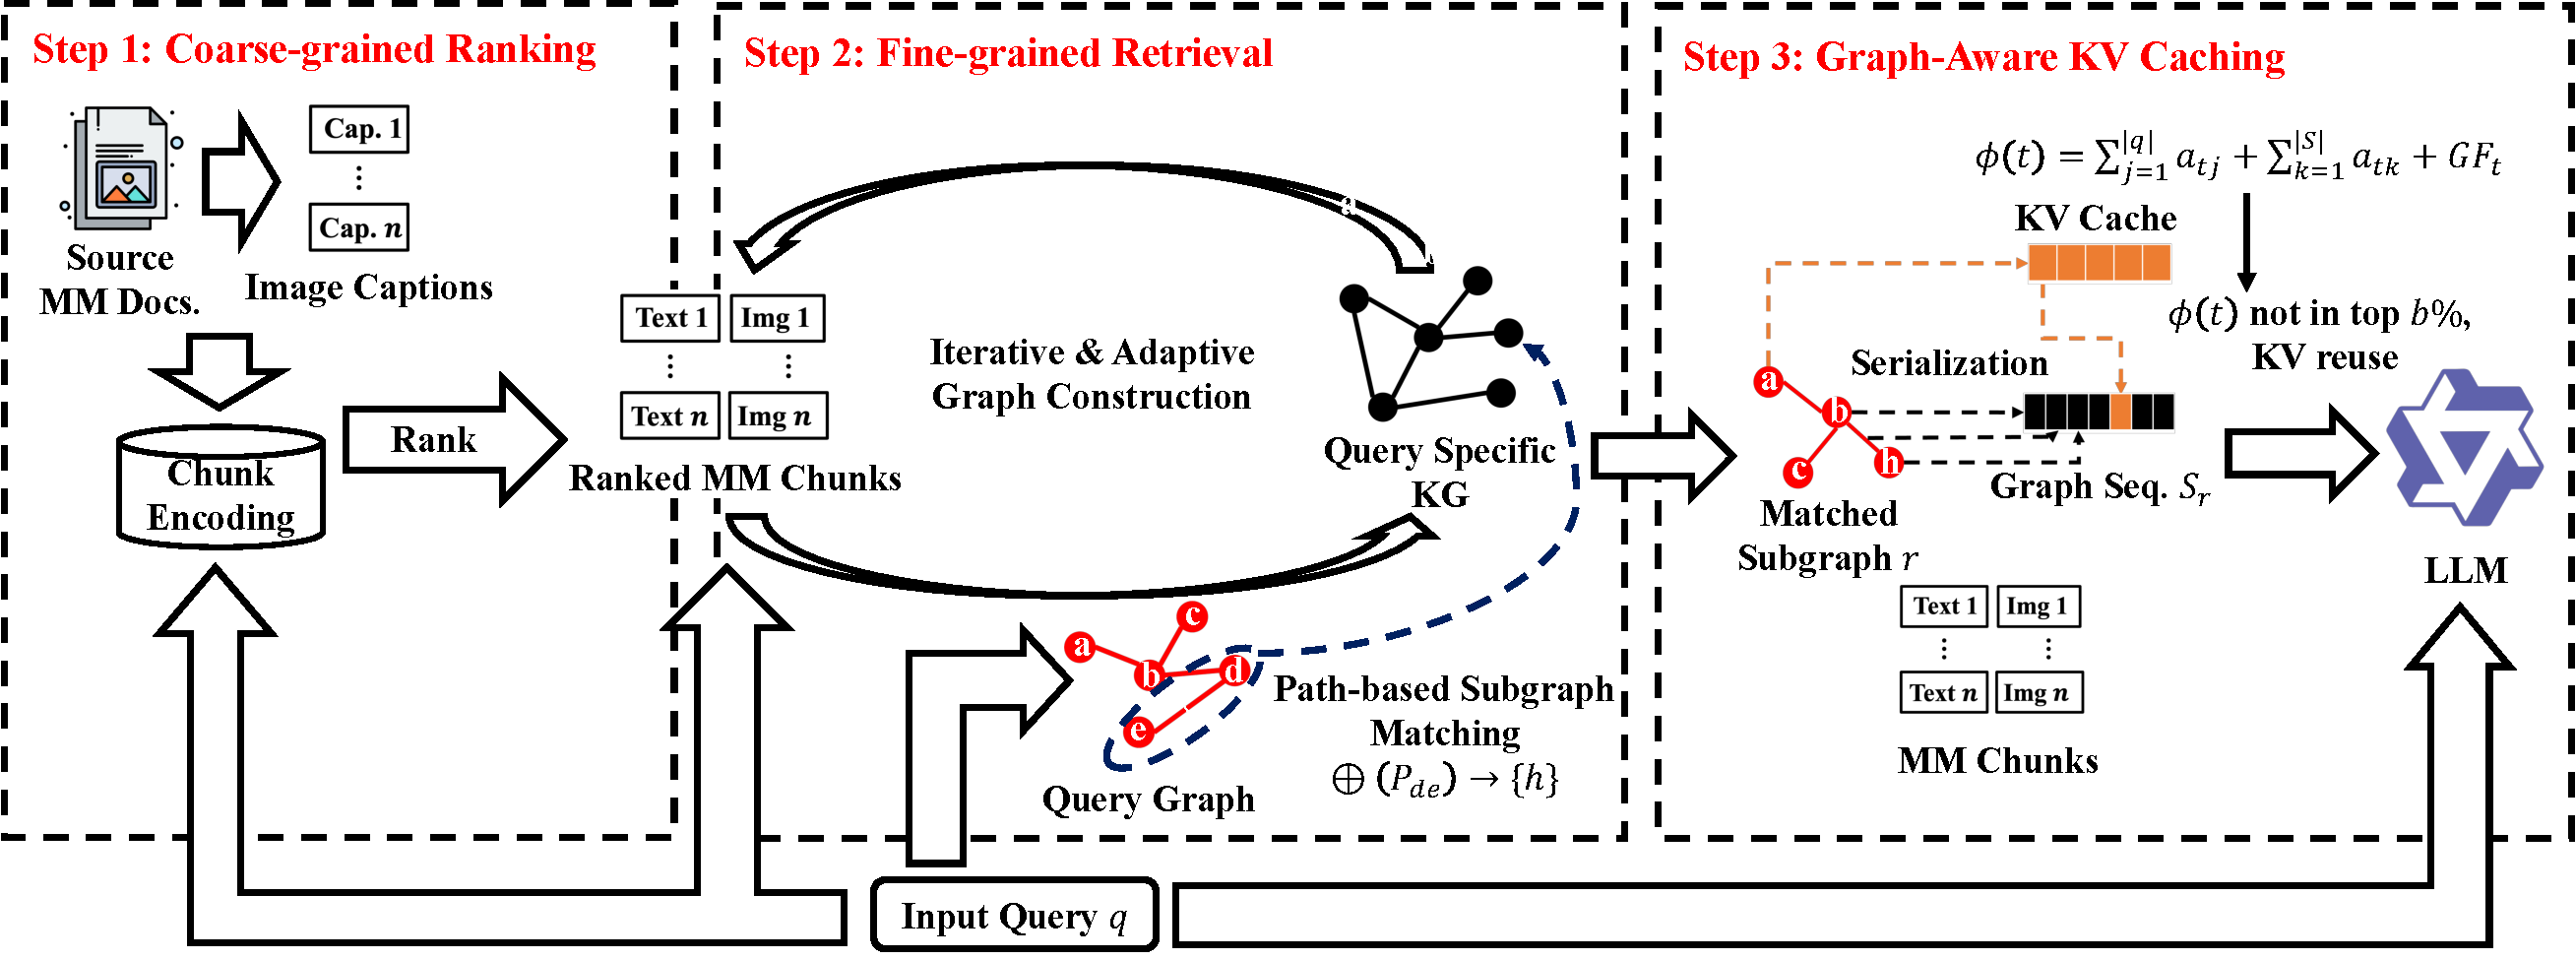
\includegraphics[width=\textwidth]{figures/mgrag/pipeline_new.pdf}
\caption{The MGRAG pipeline. Ranked chunks support incremental query-aware graph construction and path-based matching. The matched graph also supplies features for selective KV recomputation. Original Figure 2, p.~2484~\cite{mgrag-paper}.}
\label{fig:mgrag:pipeline}
\end{figure}

Two graphs serve different purposes. The query graph $\mathcal{QG}_q=(\widehat{\mathcal V}_q,\widehat{\mathcal E}_q)$ describes the entities and relations requested by $q$, including placeholders for unknown information. The evidence graph $\mathcal{KG}_q=(\mathcal V_q,\mathcal E_q)$ contains facts extracted from the chunks considered for that query. A mapping connects query entities to evidence entities. Paths between the mapped endpoints supply candidate evidence for the query relations.

For generation, MGRAG uses the graph sequence $S_r$, the original chunks $\mathcal C_q$ consumed during construction, and the query $q$. Keeping the chunks preserves access to text and visual evidence beyond the extracted triples. Their identity also links the selected graph to the material originally ranked and processed during construction. The graph gives the generator an explicit selection of relational content, while the source chunks provide the material from which the selection was made. The final multimodal context retains the original images alongside their extracted relational representation.

\section{Coarse-grained Ranking}
\label{sec:mgrag:ranking}

MGRAG first divides textual documents into overlapping chunks. The published setting uses a chunk length $l_c=256$ tokens and overlap $l_o=32$ tokens. Images form the other members of the chunk collection, giving $\mathcal C=\mathcal T\cup\mathcal D_{\mathrm{img}}$, where $\mathcal T$ denotes the text chunks. This collection is the input to the coarse retrieval stage. Ranking identifies the order in which content will be examined, rather than directly defining the final graph context.

The implementation uses the text encoder bge-base-en-v1.5~\cite{mgrag-bge_embedding}. Text chunks are encoded directly. An image is represented for ranking by its caption, which can be supplied by the dataset or generated by a language model. Both types of evidence can therefore be compared in the text embedding space. Let $\mathcal M$ denote that encoder and $\mathbf h_c$ the representation of a candidate chunk. For an image chunk, the input to $\mathcal M$ is its caption. This detail matters because the ranking representation expresses the image through language, whereas the later extraction and answering stages can use its visual content.

For a query containing text $q_{\mathrm{txt}}$ and an image caption $q_{\mathrm{cap}}$, MGRAG averages the two representations,
\begin{equation}
\mathbf h_q=\frac{\mathcal M(q_{\mathrm{txt}})+\mathcal M(q_{\mathrm{cap}})}{2}.
\label{eq:mgrag:query-embedding}
\end{equation}
A query with one modality uses its corresponding textual representation. The distance to a candidate is
\begin{equation}
 d(q,c)=\lVert\mathbf h_q-\mathbf h_c\rVert_2,
\label{eq:mgrag:distance}
\end{equation}
and the chunks are ordered by increasing distance. Equations~\ref{eq:mgrag:query-embedding} and~\ref{eq:mgrag:distance} retain the averaging and Euclidean-ranking operations of the published method.

This stage gives a query-dependent priority to relatively inexpensive chunk representations. Fine-grained processing begins with the nearest chunk and can move down the list when its current graph is insufficient. A high-ranked chunk becomes a candidate for relational extraction and subsequent matching. Conversely, graph matching can stop construction before every candidate has been processed. The coarse-to-fine design separates the cost of ordering the corpus from the cost of extracting its query-related facts.

Caption quality affects which images receive an early position. A caption can omit a visual detail that becomes relevant during graph construction, or foreground content unrelated to the query. The published CLIP substitution experiment tests an alternative coarse representation within this pipeline. Its results are discussed alongside the component ablations in Section~\ref{sec:mgrag:ablations}, where the encoder choice can be assessed under the same answering task.

\section{Query-aware Graph Construction}
\label{sec:mgrag:construction}

\subsection{Representing the query}

MGRAG asks the language model to extract entities and relations from the query. Some query entities are known, such as the name of a person or an object appearing in the question. Others are requested by the question. The extraction prompt represents those unknown components using semantically meaningful placeholders, including types such as \emph{Person} or \emph{Year}. A placeholder provides a textual representation that can be compared with evidence entities even though its value has not yet been supplied.

Figure~\ref{fig:mgrag:query-graph} shows the query and evidence graph representations. The placeholder boxes describe missing knowledge in the query. Passage nodes connect extracted entities back to their chunks. These connections let the graph carry both relational content and its association with the original multimodal evidence. In a multimodal corpus, a passage node can represent an image as well as a text chunk.

\begin{figure}[tbp]
\centering
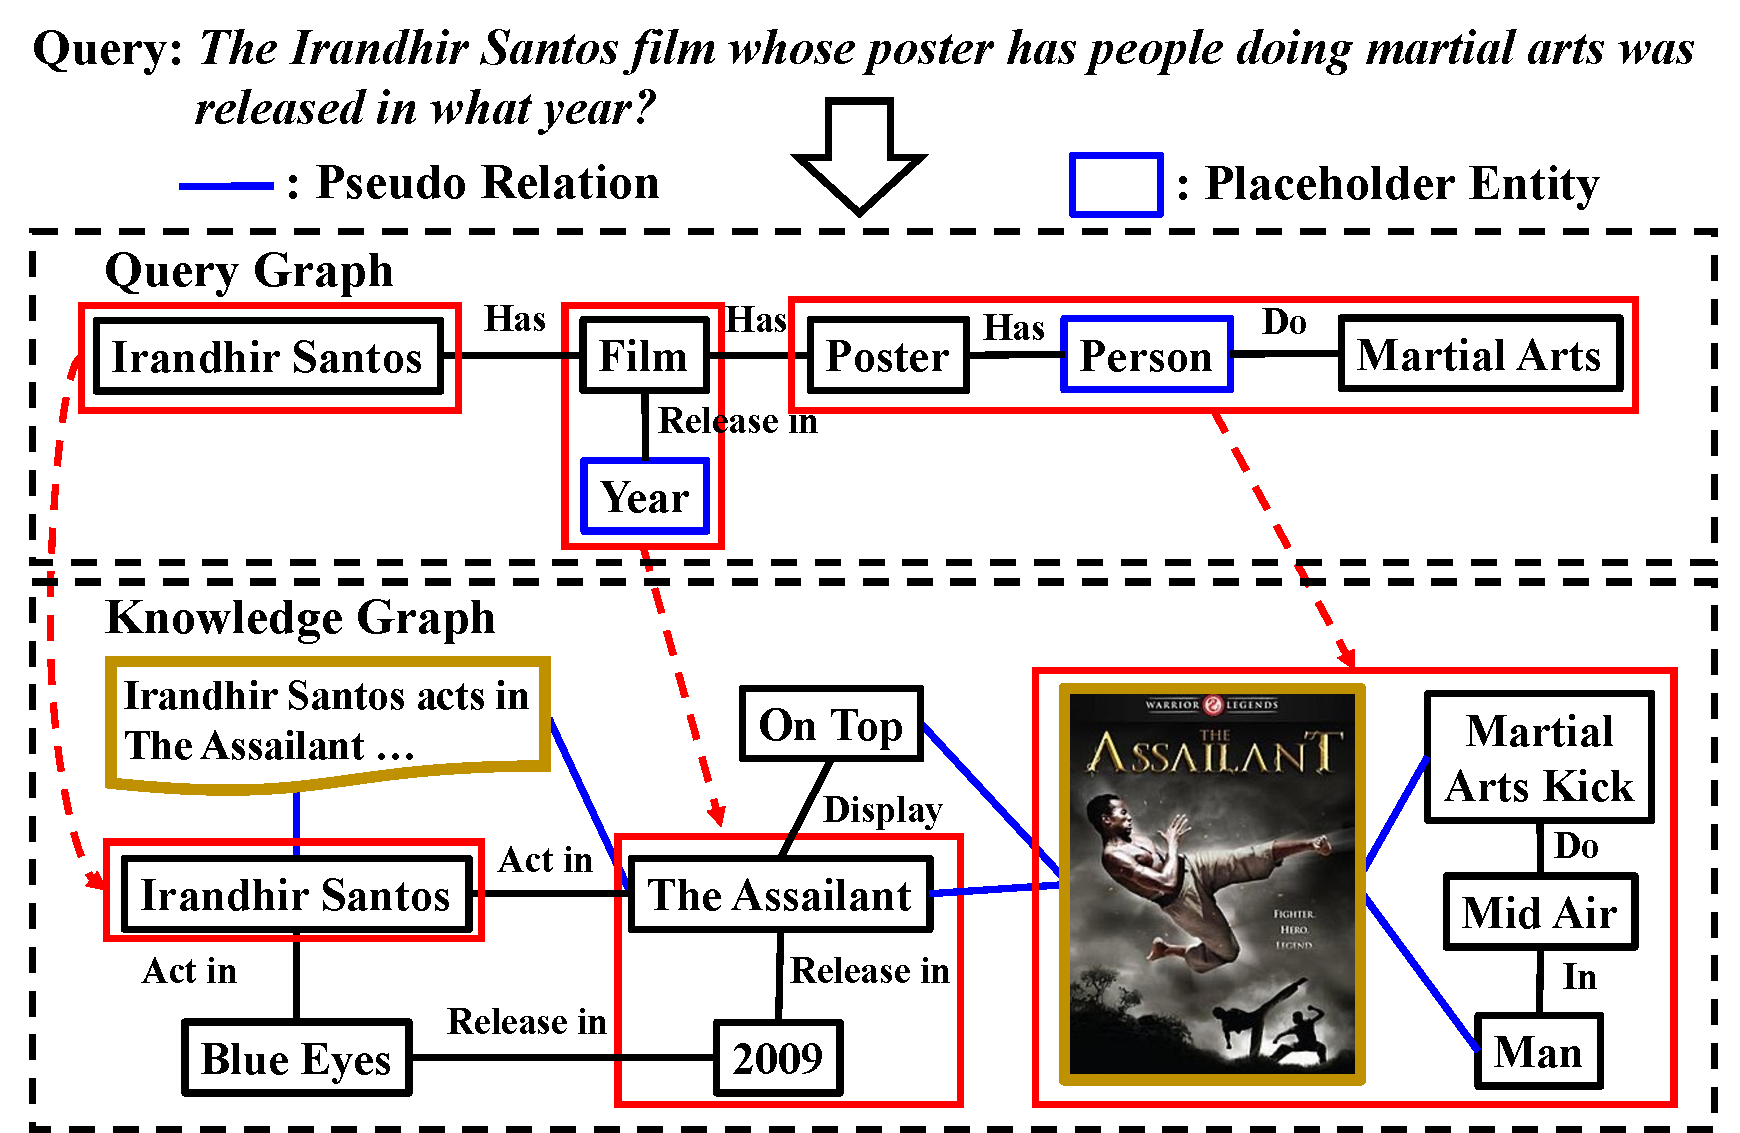
\includegraphics[width=0.95\textwidth]{figures/mgrag/query_graph.pdf}
\caption{Query and evidence graphs in path-based semantic matching. Placeholder entities express unknown query information; pseudo-relations connect passage nodes to extracted entities. Original Figure 3, p.~2485~\cite{mgrag-paper}.}
\label{fig:mgrag:query-graph}
\end{figure}

The original example asks which year an Irandhir Santos film was released when its poster shows people doing martial arts. The query graph connects the actor to an unknown film, the film to a poster, and a person on the poster to an action. It also includes a release-year requirement. The evidence graph contains named film candidates and a visual description of a man performing a martial-arts kick in midair. The depicted film, \emph{The Assailant}, is connected to the year 2009.

The example separates identifying the film from reading its release year. The actor's name alone can lead to several film candidates, including the other film shown in the graph. The visual relation supplies the condition that distinguishes the requested candidate. Once the candidate is connected to the poster evidence, the release relation provides the requested value. The query therefore needs a connected account of the actor, film, depicted action, and year. A list containing a similar actor passage and an unrelated year passage would leave that correspondence unresolved.

The placeholders give the matcher explicit locations for these missing values. The film placeholder can be compared with named film entities, while the year placeholder marks the relation whose endpoint supplies the requested answer. Representing unknown values by their semantic roles lets matching operate before those values are known. The path procedure then tests whether the selected evidence entities are connected through semantically suitable relations. This is the point at which the query's information requirement becomes a constraint on the retrieved graph.

The query graph expresses a retrieval requirement at entity and relation granularity. Its construction is a model-mediated interpretation of the question. The downstream matcher operates on this interpretation, including the wording chosen for placeholders and relations. A semantic match therefore indicates agreement between the represented query and represented evidence. Answer quality is evaluated separately using the original question and reference answer.

\subsection{Extracting facts from ranked chunks}

For a chunk $c$, the extraction model receives the chunk, query, and extraction prompt $p_{\mathrm{ext}}$. Its output contains query-related entities and relations,
\begin{equation}
 (\mathcal V_q^c,\mathcal E_q^c)
 =\operatorname{LLM}(c,q,p_{\mathrm{ext}}).
\label{eq:mgrag:extraction}
\end{equation}
Including $q$ makes the extraction selective. The model is asked to identify events and relations relevant to the current question, rather than to enumerate every describable fact in the chunk. For an image, this permits attention to query-related visual events; for text, it permits selection of the entities and relationships needed to describe the requested evidence.

The chunk is also added as a passage node. MGRAG connects this node to the entities extracted from it using the pseudo-relation \texttt{consists\_in}, retaining the published relation name and orientation from chunk to entity. If $\mathcal C_q^{(i)}$ is the prefix of ranked chunks consumed after iteration $i$, the cumulative graph contains
\begin{align}
 \mathcal V_q^{(i)}
 &=\bigcup_{c\in\mathcal C_q^{(i)}}(\mathcal V_q^c\cup\{c\}),\\
 \mathcal E_q^{(i)}
 &=\bigcup_{c\in\mathcal C_q^{(i)}}\left(\mathcal E_q^c\cup
 \{(c,\texttt{consists\_in},v):v\in\mathcal V_q^c\}\right).
\label{eq:mgrag:graph-union}
\end{align}
The iteration-indexed notation makes explicit that the unions range over the chunks already processed. 

Passage nodes give the matcher a route between a fact and its context. They can also connect facts associated with the same source item. The resulting graph combines extracted semantic relations with document-membership relations. These two edge types have different interpretations, even though both participate in the evidence representation. The distinction is visible in the original example's use of separate edge colors.

\subsection{Matching as a stopping decision}

After each graph update, MGRAG attempts path-based semantic subgraph matching against the query graph. A valid match ends the construction loop. If the matcher returns an empty result, the next ranked chunk is used to enrich the graph. The loop is bounded by the maximum number of construction iterations $\mu$. Thus, the amount of graph construction depends on both the ranking order and the matching outcome.

This design uses semantic coverage as an operational stopping test. Coverage is evaluated through the query graph's entities and relations, so a match requires more than one highly similar isolated entity. The procedure seeks a correspondence for the query's relational requirements. When the current graph lacks such a correspondence, additional evidence can introduce a missing endpoint, a relation, or a path between existing endpoints. The graph can therefore become matchable through information accumulated across chunks.

The iteration cap controls the amount of evidence examined. It also bounds the opportunity to recover a fact that occurs late in the ranking. Reaching the cap and finding a valid match are distinct termination events. The matcher returns an empty result when its search finds no valid correspondence in the current graph. The cap, graph extraction, and matching threshold jointly determine which context reaches the answer generator.

\section{Path-based Semantic Subgraph Matching}
\label{sec:mgrag:matching}

\subsection{From edges to paths}

A relation in the query graph can be expressed by several relations in the evidence graph. MGRAG assigns text embeddings to entity and relation descriptions. For a path $P(u,v)$ containing relations $r_1,\ldots,r_k$, it defines a semantic representation by aggregating the relation embeddings,
\begin{equation}
 \mathbf h_{P(u,v)}=\bigoplus_{j=1}^{k}\mathbf h_{r_j}.
\label{eq:mgrag:path-embedding}
\end{equation}
The aggregation operator can use mean pooling. This operation provides a representation of the composed evidence relation that can be compared with a query relation. The published greedy expansion further evaluates a joint representation containing the current path, candidate edge, and candidate endpoint. These are the path representation and extension test used at different steps of the procedure.

Let $I:\widehat{\mathcal V}_q\rightarrow\mathcal V_q$ be a candidate entity mapping. For a query edge $(u,\widehat r,v)$, the candidate evidence paths run from $I(u)$ to $I(v)$. Denote this collection by $\mathcal P(I(u),I(v))$. The matching objective is
\begin{equation}
\max_I\ \sum_{(u,\widehat r,v)\in\widehat{\mathcal E}_q}
 \max_{P\in\mathcal P(I(u),I(v))}
 \cos(\mathbf h_{\widehat r},\mathbf h_P).
\label{eq:mgrag:matching-objective}
\end{equation}
Candidate mappings must satisfy the semantic threshold $\theta$ for the mapped entities and for every query relation's supporting path,
\begin{align}
 \cos(\mathbf h_u,\mathbf h_{I(u)})&>\theta
 &&\text{for all }u\in\widehat{\mathcal V}_q,\\
 \max_{P\in\mathcal P(I(u),I(v))}\cos(\mathbf h_{\widehat r},\mathbf h_P)&>\theta
 &&\text{for all }(u,\widehat r,v)\in\widehat{\mathcal E}_q.
\label{eq:mgrag:matching-constraints}
\end{align}
The constraints validate each query edge against an associated evidence path. The selected evidence is the subgraph formed from the mapped entities and accepted paths, which can include intermediate entities absent from the query graph.

For a fixed candidate mapping, the inner maximization in Equation~\ref{eq:mgrag:matching-objective} selects a supporting path for each query relation. The outer search compares entity mappings after those relation scores have been obtained. These levels distinguish the problem of locating the query's entities from the problem of explaining their relationships. Two mappings can have similar endpoint embeddings yet differ in whether their connecting paths satisfy the requested relation. Conversely, several paths between the same mapped endpoints can express different relations and receive different semantic scores.

The returned subgraph is assembled from the paths needed by the accepted query edges. Paths can share intermediate entities and edges. Their union exposes those shared facts in the evidence graph, while the query graph continues to specify which relational requirements were validated. A graph assembled in this way need not have the same number of entities as the query graph. Intermediate evidence nodes are precisely what permits a relation expressed compactly in the question to be supported by a more detailed description in the corpus.

This representation relaxes the requirement that the two graphs express a fact with the same number of edges. In the family-relation example, the evidence path has two steps and the query relation has one. Their correspondence is judged through semantic similarity. The procedure retains endpoint requirements, so the selected relation must connect entities that themselves correspond to the query. It combines entity-level alignment with path-level evidence instead of treating either component as sufficient on its own.

\subsection{Anchor selection and candidate mappings}

MGRAG first computes pairwise cosine similarities between query entities and evidence entities. The highest-similarity pair supplies an anchor entity in the query graph and its candidate counterpart in the evidence graph. If no valid match is obtained from that anchor, the method tries other anchors. For the selected query anchor, Algorithm~\ref{alg:mgrag:matching} considers each evidence counterpart exceeding the threshold and enumerates mappings consistent with that correspondence.

Candidate mappings are enumerated using a similarity-based modification of VF2~\cite{mgrag-cordella2004sub}. VF2 supplies a graph-matching search procedure; the MGRAG adaptation uses the threshold $\theta$ in semantic feasibility checks. Each candidate is then validated relation by relation through greedy path search. A candidate entity correspondence can consequently be rejected because one of its required relations lacks an acceptable evidence path.

For each accepted mapping, the algorithm takes the union of the paths that support its query edges. It averages the edge-wise semantic similarities to obtain a score $s$. The highest-scoring accepted subgraph is returned. Dividing by the number of query edges does not change the ranking of candidate mappings for the same query. It provides an average semantic score with a common range across queries whose graph sizes differ.

\begin{algorithm}[tbp]
\caption{Path-based semantic matching in MGRAG}
\label{alg:mgrag:matching}
\begin{algorithmic}[1]
\REQUIRE Query graph $\mathcal{QG}_q$, query anchor $\gamma$, evidence graph $\mathcal{KG}_q$, threshold $\theta$
\STATE Initialize valid results $\mathcal R\gets\varnothing$
\FOR{each $v_a\in\mathcal V_q$ with $\cos(\mathbf h_{v_a},\mathbf h_\gamma)>\theta$}
\STATE Enumerate candidate mappings consistent with $I(\gamma)=v_a$
\FOR{each candidate mapping $I$}
\STATE Initialize the subgraph with mapped query entities; set $s\gets0$
\FOR{each query edge $(u,\widehat r,v)$}
\STATE Search greedily for a semantically valid path from $I(u)$ to $I(v)$
\IF{the path search fails}
\STATE Reject $I$ and stop validating this mapping
\ELSE
\STATE Add the path's nodes and edges to the candidate subgraph
\STATE Add its cosine similarity to $s$
\ENDIF
\ENDFOR
\IF{every query edge has a valid path}
\STATE Add the subgraph and score $s/|\widehat{\mathcal E}_q|$ to $\mathcal R$
\ENDIF
\ENDFOR
\ENDFOR
\STATE Return the highest-scoring result, or $\varnothing$ if $\mathcal R$ is empty
\end{algorithmic}
\end{algorithm}

\subsection{Greedy semantic path growth}

The path search begins at the mapped source entity and maintains its current endpoint $x$. For each neighboring entity $y$ and connecting edge $(x,r,y)$, MGRAG evaluates the candidate extension using
\begin{equation}
 \cos\!\left(\mathbf h_P\oplus\mathbf h_{e(x,r,y)}\oplus\mathbf h_y,
 \mathbf h_{\widehat e(u,\widehat r,v)}\right).
\label{eq:mgrag:greedy-score}
\end{equation}
Among extensions exceeding $\theta$, it selects the highest-scoring one, appends that edge to the path, and updates the endpoint to $y$. This repeats until the path reaches the mapped target. The search fails when no qualifying extension is available. The experiments also impose a maximum path length $l_p$ to bound expansion.

The endpoint and threshold checks serve different roles. Reaching the target gives the evidence path the required relational endpoints. Passing the semantic checks gives it a representation consistent with the requested relation. An attractive local extension can still prevent the greedy search from reaching the target, so a failed search does not establish that all possible paths fail. The algorithm returns the best result among the valid candidates it finds.

All query edges must pass path validation before a mapping is accepted. This condition prevents a single high-scoring relation from compensating for an unsupported required relation. The selected subgraph may contain paths of different lengths, because the evidence required by different query edges can have different decompositions. Construction then stops on that accepted match; otherwise, a further ranked chunk is incorporated and matching is attempted again.

\subsection{Published algorithmic properties}

The publication states that path-based semantic subgraph matching is NP-hard. Its proof sketch reduces subgraph isomorphism to a restricted instance with uniform embeddings and unit path lengths. The result motivates the use of semantic path growth and constrained mapping enumeration. The complexity of enumerating mappings remains relevant even when each individual extension is selected greedily.

The published Theorem 2 gives a threshold-based quality condition for a valid returned match. Every matched query relation has a supporting path with cosine similarity at least $\theta$. Under the strict acceptance test in Equation~\ref{eq:mgrag:matching-constraints}, the average score of an accepted mapping exceeds $\theta$ as well. This condition describes the semantic validation of returned evidence. It is conditional on finding a valid match and does not require the algorithm to recover one whenever such a subgraph exists.

The technical report discusses the threshold in terms of a bottleneck transport cost~\cite{mgrag-tech-report}. With a per-edge cost of one minus cosine similarity, the threshold limits the largest accepted local cost. The explicit theorem statement in the publisher PDF is used here to specify the result. The method's empirical quality is assessed by the graph-matching substitutions and answer-quality measurements in Section~\ref{sec:mgrag:results}.

\subsection{Serializing selected evidence}

After matching, MGRAG serializes the selected triples into $S_r$, separating facts with \texttt{[SEP]}. This sequence is combined with $q$ and the original chunks consumed during construction. The serialization supplies an explicit list of entities and relationships to the answering model. Original chunks remain available because extraction is a selective description of the evidence, and some linguistic or visual details may lie outside the triples.

The same entities and relations were involved in the earlier graph-construction calls. Their tokens can therefore overlap with tokens in the answering context. MGRAG uses this relationship to reuse cached computation from construction while updating states important to the new answering context. The graph produced during retrieval thus becomes an input to the context-computation policy as well as to the language model's prompt.

\section{Graph-aware KV Recomputation}
\label{sec:mgrag:cache}

\subsection{Reuse and selective updates}

A transformer caches key and value projections so that earlier token states can be reused. In MGRAG, content processed during graph construction appears again in the query-answering context. Recomputing every state repeats part of this work. Reusing every state can retain representations calculated under a different surrounding sequence. The cache policy chooses a subset for recomputation and reuses the others.

Let $\phi(t)$ be the recomputation score of token $t$. At each transformer layer, MGRAG recomputes the tokens in the highest $b\%$ of scores and reuses the cached states for the remaining tokens. The published description uses a fixed-size cache with least-recently-used eviction. Its proposed policy concerns the ranking of token states for selective recomputation. The budget is represented by $b$; the numerical experiment tables do not specify a fixed value for that budget.

Figure~\ref{fig:mgrag:cache} shows how the graph contributes. Query-related events are represented by entities and relations. The score combines attention to the query, attention to the graph sequence, and a feature derived from the topology of the associated fact. The goal of the added term is to give tokens access to an event-level structural signal alongside token-level attention.

\begin{figure}[tbp]
\centering
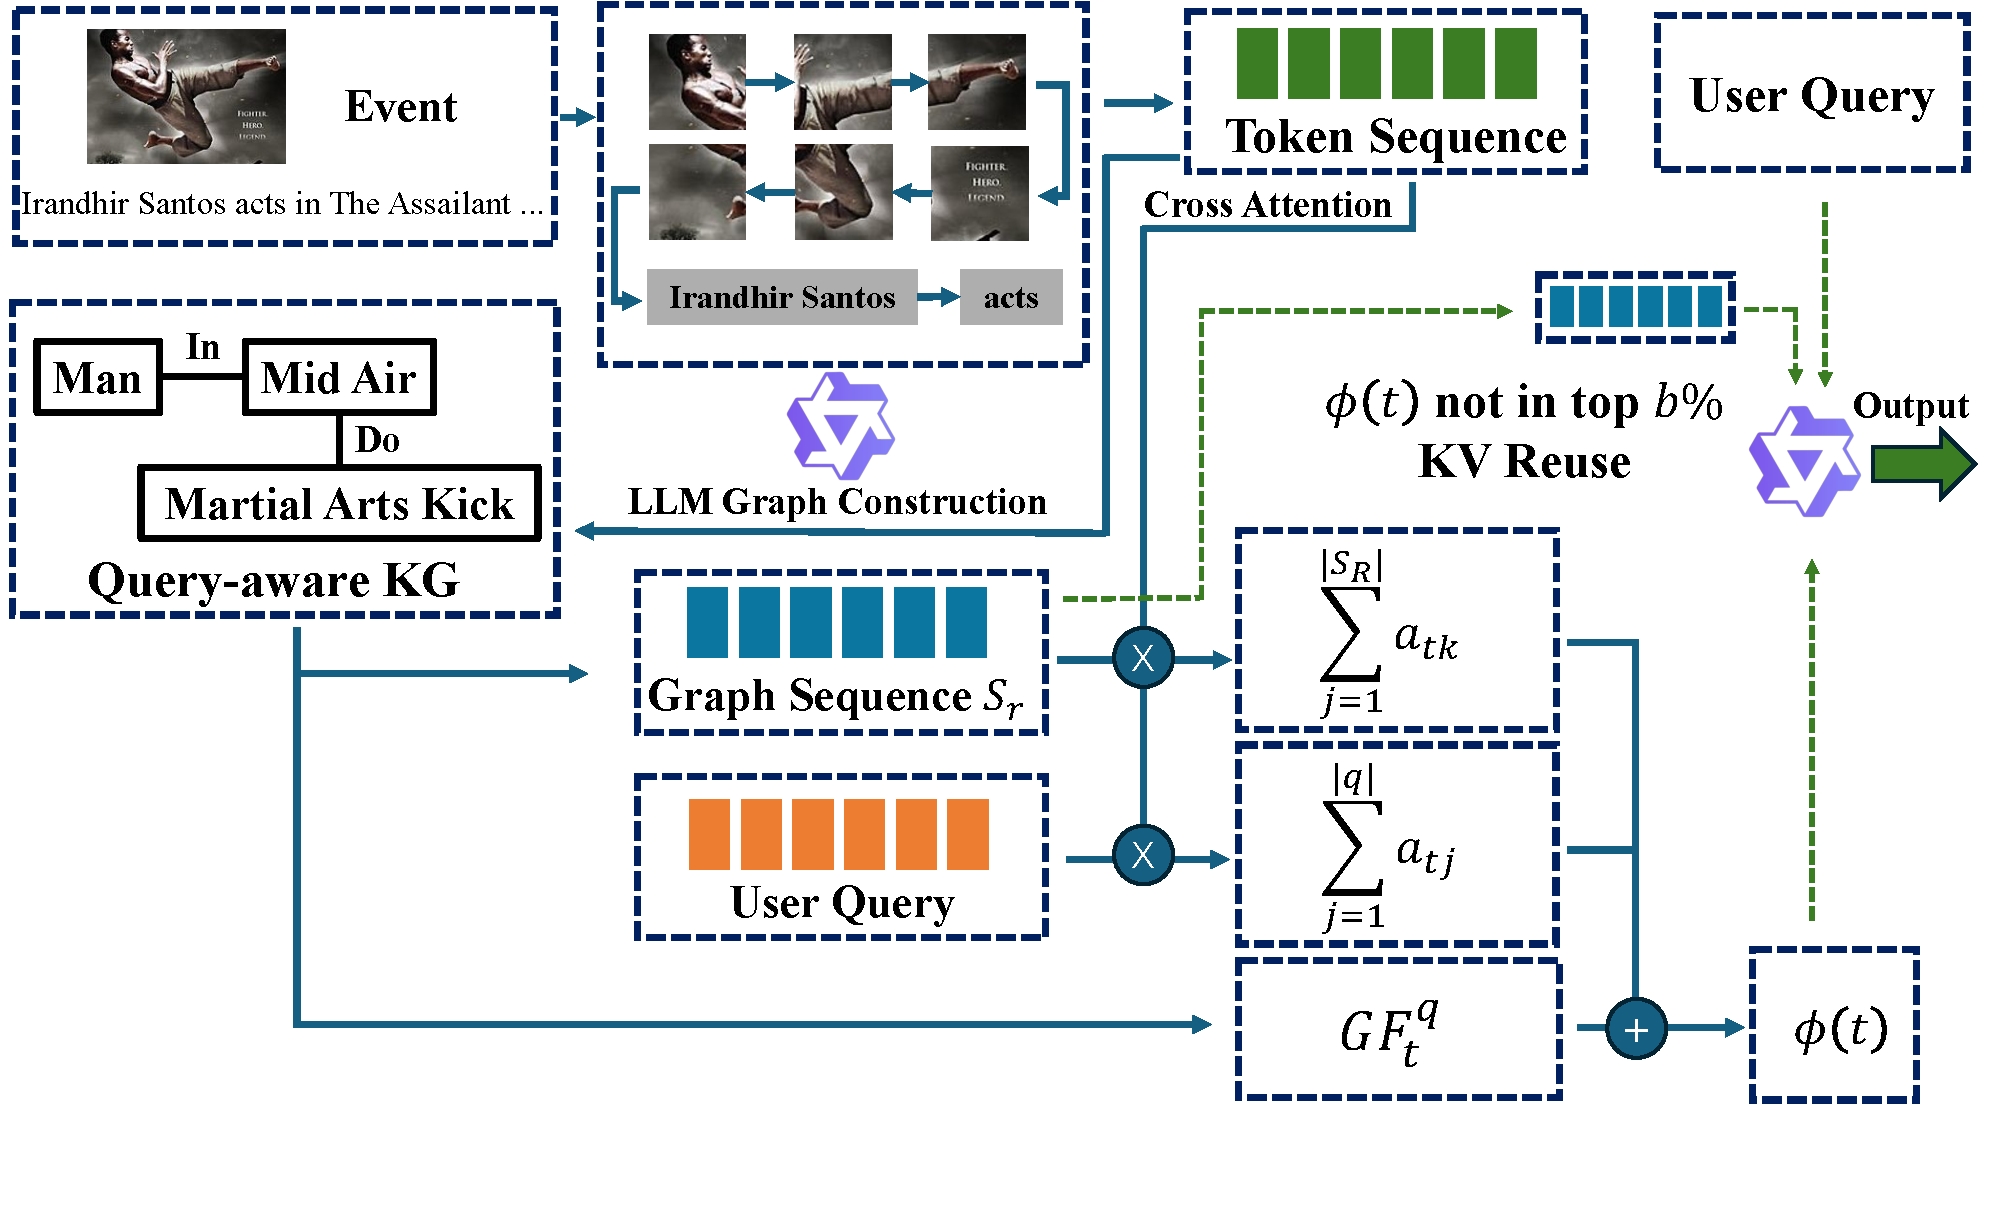
\includegraphics[width=0.95\textwidth]{figures/mgrag/graph_based_cache.pdf}
\caption{Graph features supplement attention in token recomputation scoring. The diagram retains the original graphical content. Original Figure 4, p.~2487~\cite{mgrag-paper}.}
\label{fig:mgrag:cache}
\end{figure}

\subsection{Topological features of facts}

MGRAG uses degree, betweenness, eigenvector, and closeness centrality to characterize a node. Degree centrality measures its normalized number of adjacent connections. Betweenness characterizes its participation in paths connecting other nodes. Eigenvector centrality weights connections by the centrality of their neighbors. Closeness uses distances to other graph nodes. The published method averages these four quantities,
\begin{equation}
 f(u)=\frac{dc(u)+bc(u)+ec(u)+cc(u)}{4}.
\label{eq:mgrag:node-feature}
\end{equation}
For a token associated with a triple $(u,r,v)$, its graph feature is the mean of the endpoint scores,
\begin{equation}
 GF_t^q=\frac{f(u)+f(v)}{2}.
\label{eq:mgrag:token-feature}
\end{equation}
The token-to-fact association follows the entity and relation token spans in the serialized representation. Tokens referring to the same fact therefore receive a shared structural component.

The graph feature concerns an entity's position in the query-specific graph. A node that connects several extracted facts can carry a different score from an isolated endpoint. Because extraction is query-dependent, the feature is calculated from a representation already selected for that query. Its meaning is relational importance within that graph, rather than a corpus-wide importance measure.

The published graphs are small, with fewer than twenty entities on average according to the report. Averaging four graph statistics provides a direct structural feature for these graphs. The recomputation score uses graph and attention information available during processing.

\subsection{Combined recomputation score}

Let $a_{tj}$ denote attention between token $t$ and token $j$, and let $|q|$ and $|S_r|$ denote the query and serialized-graph lengths. The score is
\begin{equation}
 \phi(t)=\sum_{j=1}^{|q|}a_{tj}
       +\sum_{k=1}^{|S_r|}a_{tk}+GF_t^q.
\label{eq:mgrag:cache-score}
\end{equation}
The first term expresses interaction with the current question. The second expresses interaction with the selected relational context. The third assigns the structural feature of the associated graph fact. The resulting sum determines which token states consume the recomputation budget.

The publication compares the policy with vLLM prefix caching~\cite{mgrag-kwon2023efficient} and CacheBlend~\cite{mgrag-yao2025cacheblend}. Their retrieval pipelines and cache variants are identified separately in the evaluation. The inverse ablations also evaluate graph-aware recomputation within an existing retrieval pipeline. These comparisons expose answer-quality and time changes under several compositions of retrieval and caching.

\section{Computational Cost}
\label{sec:mgrag:complexity}

The published offline encoding cost is $O(|\mathcal C|d_{\mathrm{emb}}l_c^2)$, with embedding dimension $d_{\mathrm{emb}}$. Using $k$ processed chunks, query-graph vertex and edge sets $\widehat{\mathcal V}$ and $\widehat{\mathcal E}$, evidence-graph sets $\mathcal V$ and $\mathcal E$, maximum path length $l_p$, and language-model hidden dimension $d_{\mathrm{LLM}}$, its reported online bound is
\begin{equation}
\begin{split}
 O\bigl(&d_{\mathrm{emb}}kl_c^2
 +l_p|\widehat{\mathcal E}|\,|\mathcal V|^{|\widehat{\mathcal V}|+1}
 +|\mathcal V||\mathcal E|\\
 &+d_{\mathrm{LLM}}(|S_r|^2+|q|^2)\bigr).
\end{split}
\label{eq:mgrag:complexity}
\end{equation}
The mapping-enumeration term is exponential in query-graph size. Query-specific construction and a bounded path length restrict the graphs processed in the evaluated setting. Actual module costs provide the complementary evidence about where runtime is spent. In particular, graph construction calls the language model repeatedly, whereas matching operates on the extracted graph. Section~\ref{sec:mgrag:cost-results} reports these costs individually.

\section{Experimental Protocol}
\label{sec:mgrag:protocol}

The evaluation uses MMQA~\cite{mgrag-talmor2021multimodalqa} and the Arxiv, Manual, Web, Wiki, Wit, and Recipe subsets of MRAMG-Bench~\cite{mgrag-yu2025mramg}. Table~\ref{tab:mgrag:datasets} preserves the published dataset statistics. MMQA includes textual and image queries. The six MRAMG subsets contain textual queries over multimodal corpora. Their query-hop ranges and corpus sizes differ, so results are reported by dataset.

\begin{table}[!htbp]
\centering
\small
\setlength{\tabcolsep}{3pt}
\caption{Evaluation datasets, reproduced from published Table 3, p.~2488~\cite{mgrag-paper}. T and I denote textual and image query modalities. The columns comprise MMQA and six MRAMG subsets.}\label{tab:mgrag:datasets}
\begin{tabular}{lccccccc}
\toprule
Statistic & MMQA & Wiki & Wit & Recipe & Arxiv & Manual & Web\\
\midrule
Query Modality     & T / I       & T             & T            & T               & T              & T               & T             \\
Queries            & 951           & 500           & 600          & 2,360            & 200            & 390             & 750           \\
Texts              & 218,285       & 538           & 639          & 1,528           & 101            & 40              & 1,500         \\
Images             & 57,058        & 538           & 639          & 8,569           & 337            & 2,607           & 1,500         \\
Corpus Size             & 22.5M        & 680k           & 478k          & 1.1M           & 136k            & 420k           & 215k         \\
Query Hops             & 1--2        & 2--5           & 2--4          & 1--6           & 3--4            & 2--6           & 2--3         \\
Avg Query Hops 	   & 1.5           & 3.0           & 2.8          & 3.3             & 3.1            & 3.7             & 2.4           \\
\bottomrule
\end{tabular}
\end{table}


The shared generation backbone is Qwen2.5-VL-7B-Instruct~\cite{mgrag-bai2025qwen2}. The experiments run on an Intel Xeon Gold 5220R CPU at 2.20 GHz and one NVIDIA A100-SXM4 GPU with 40 GB memory. The retrieval amount is set to five, text chunks use 256 tokens, and overlap is 32 tokens. HippoRAG2 uses Contriever for dense passage retrieval~\cite{mgrag-izacardunsupervised}; the other reported embedding configurations use bge-base-en-v1.5. Similarity-based retrieval represents images through their captions. These are the published controls for the comparisons in this chapter.

VanillaRAG is implemented with LangChain and FAISS~\cite{mgrag-douze2024faiss}. The GraphRAG implementation is nano-graphrag~\cite{mgrag-nanographrag}, and the remaining baseline systems use their released implementations. The protocol selects hybrid search for LightRAG and local search for GraphRAG. vLLM accelerates the tested baseline systems, while MGRAG uses its graph-aware cache procedure. Other baseline hyperparameters follow the implementations' defaults.

Four metrics characterize answers. Semantic similarity (SIM.) is the cosine similarity between bge-base-en-v1.5 representations of generated and reference answers. Accuracy (ACC.) is the reported proportion of correct answers. ROUGE-L (ROG.) evaluates longest-common-subsequence overlap~\cite{mgrag-lin2004rouge}, and BLEU-1 evaluates modified unigram precision~\cite{mgrag-papineni2002bleu}. The paper uses the RAGAS evaluation framework~\cite{mgrag-es2024ragas}. The tables preserve its metric names and precision, including the label BLEU used for BLEU-1.

The four answer metrics reflect different properties. Embedding similarity compares semantic proximity at the answer level. ROUGE-L and BLEU-1 retain sensitivity to the wording shared with the reference. Accuracy provides the task's correctness measurement. They are shown together because agreement in one measure does not imply identical behavior in the others. The publication reports point estimates for these experiments.

The complete-system baselines use different retrieval units. VanillaRAG returns dense-retrieved chunks, and R1-Searcher incorporates reinforcement learning into search and question answering. GraphRAG organizes its graph into communities and prepares summaries; LightRAG retrieves graph elements and neighborhoods through its selected search mode. HippoRAG2 adds passage nodes and uses Personalized PageRank for retrieval. In the published experiment, these systems are compared as implemented pipelines. Their results include their own indexing and evidence-selection choices, while the shared backbone and evaluation metrics provide the common answering conditions.

Component substitutions evaluate graph construction, semantic matching, and cache policy within MGRAG. Inverse ablations add matching and recomputation to other retrieval systems.

\section{Answer Quality and Structural Retrieval}
\label{sec:mgrag:results}

\subsection{Complete-system comparisons}

Table~\ref{tab:mgrag:main} reproduces the complete-system results. MGRAG has the highest reported value in each of the four metric rows for each dataset. On MMQA, its accuracy is 0.7442, compared with 0.7053 for VanillaRAG and 0.6335 for HippoRAG2. Its semantic similarity is 0.8533, ROUGE-L is 0.6763, and BLEU-1 is 0.7215. GraphRAG and LightRAG have missing MMQA entries because those experiments exceeded three days. The dash records the time limit and supplies no quality measurement for those systems.

{\small
\setlength{\tabcolsep}{3pt}
\begin{longtable}{llrrrrrr}
\caption{Answer quality with Qwen2.5-VL-7B-Instruct, reproduced from published Table 4, p.~2489~\cite{mgrag-paper}. Vanilla., R1., Graph., Light., and Hippo. denote VanillaRAG, R1-Searcher, GraphRAG, LightRAG, and HippoRAG2. A dash means that the experiment exceeded three days; it is not a zero score. Bold and underlining retain the publication's highlighting.}\label{tab:mgrag:main}\\
\toprule
Dataset & Metric & Vanilla. & R1. & Graph. & Light. & Hippo. & MGRAG\\
\midrule\endfirsthead
\multicolumn{8}{c}{\tablename\ \thetable\ (continued)}\\
\toprule
Dataset & Metric & Vanilla. & R1. & Graph. & Light. & Hippo. & MGRAG\\
\midrule\endhead
\bottomrule\endfoot
MMQA & SIM. & 0.8362 & 0.5478 & - & - & \underline{0.8381} & \textbf{0.8533} \\
MMQA & ACC. & \underline{0.7053} & 0.3567 & - & - & 0.6335 & \textbf{0.7442} \\
MMQA & ROG. & 0.5942 & 0.1041 & - & - & \underline{0.6659} & \textbf{0.6763} \\
MMQA & BLEU & \underline{0.6645} & 0.0817 & - & - & 0.5917 & \textbf{0.7215} \\
Arxiv & SIM. & \underline{0.8664} & 0.7051 & 0.7943 & 0.7404 & 0.8293 & \textbf{0.8760} \\
Arxiv & ACC. & \underline{0.6638} & 0.3775 & 0.2350 & 0.3813 & 0.4688 & \textbf{0.6800} \\
Arxiv & ROG. & \underline{0.2713} & 0.1189 & 0.1553 & 0.1580 & 0.2331 & \textbf{0.2726} \\
Arxiv & BLEU & \underline{0.2452} & 0.1092 & 0.1690 & 0.1370 & 0.1281 & \textbf{0.2498} \\
Manual & SIM. & \underline{0.8166} & 0.6046 & 0.5453 & 0.7255 & 0.6852 & \textbf{0.8221} \\
Manual & ACC. & \underline{0.5881} & 0.2071 & 0.1436 & 0.4096 & 0.2641 & \textbf{0.6173} \\
Manual & ROG. & \underline{0.3509} & 0.1078 & 0.0974 & 0.1595 & 0.2047 & \textbf{0.3839} \\
Manual & BLEU & \underline{0.2767} & 0.0740 & 0.0718 & 0.1385 & 0.1314 & \textbf{0.3093} \\
Web & SIM. & \underline{0.6937} & 0.6620 & 0.5470 & 0.5513 & 0.5642 & \textbf{0.7009} \\
Web & ACC. & \underline{0.4703} & 0.4200 & 0.1053 & 0.2000 & 0.3607 & \textbf{0.5123} \\
Web & ROG. & \underline{0.1508} & 0.1142 & 0.1133 & 0.0905 & 0.0616 & \textbf{0.1664} \\
Web & BLEU & 0.0326 & 0.0785 & \underline{0.1031} & 0.0206 & 0.0133 & \textbf{0.1456} \\
Wiki & SIM. & \underline{0.8824} & 0.5478 & 0.6966 & 0.7517 & 0.8204 & \textbf{0.8838} \\
Wiki & ACC. & \underline{0.7800} & 0.3567 & 0.2000 & 0.3660 & 0.6500 & \textbf{0.7845} \\
Wiki & ROG. & \underline{0.3559} & 0.1418 & 0.1361 & 0.2008 & 0.3042 & \textbf{0.3579} \\
Wiki & BLEU & \underline{0.3053} & 0.1146 & 0.1007 & 0.1863 & 0.1851 & \textbf{0.3174} \\
Wit & SIM. & \underline{0.7851} & 0.6110 & 0.6211 & 0.6973 & 0.7230 & \textbf{0.8033} \\
Wit & ACC. & \underline{0.6675} & 0.6017 & 0.1500 & 0.2483 & 0.5138 & \textbf{0.6967} \\
Wit & ROG. & \underline{0.3255} & 0.1307 & 0.1319 & 0.2416 & 0.2712 & \textbf{0.3589} \\
Wit & BLEU & \underline{0.2095} & 0.0934 & 0.1142 & 0.1928 & 0.1200 & \textbf{0.2382} \\
Recipe & SIM. & \underline{0.8599} & 0.6155 & 0.8166 & 0.8118 & 0.7792 & \textbf{0.8673} \\
Recipe & ACC. & \underline{0.6525} & 0.2180 & 0.2771 & 0.3334 & 0.4917 & \textbf{0.6814} \\
Recipe & ROG. & \underline{0.3714} & 0.1065 & 0.1745 & 0.2128 & 0.3303 & \textbf{0.4220} \\
Recipe & BLEU & \underline{0.2599} & 0.0773 & 0.1527 & 0.1648 & 0.1941 & \textbf{0.3102} \\
\end{longtable}
}


The advantage over the strongest baseline varies by dataset and metric. On Wiki, accuracy is 0.7845 for MGRAG and 0.7800 for VanillaRAG, while their semantic similarities are 0.8838 and 0.8824. On Web, the corresponding accuracies are 0.5123 and 0.4703. On Recipe, MGRAG reports ROUGE-L of 0.4220 compared with 0.3714 for VanillaRAG.

Several graph-based baselines score below VanillaRAG in this multimodal protocol. For example, on Manual, GraphRAG, LightRAG, and HippoRAG2 report accuracies of 0.1436, 0.4096, and 0.2641, compared with VanillaRAG's 0.5881. The presence of a graph by itself therefore does not predict the ranking in this table. MGRAG's results concern its specific construction, matching, and context-processing design. The substitutions below help identify which parts contribute under the same evaluation framework.

\subsection{Construction and matching substitutions}

Table~\ref{tab:mgrag:matching} reorganizes every value from the published graph-construction and matching comparison. Stanford OpenIE~\cite{mgrag-angeli2015leveraging} and the statistical extraction alternative STAT replace the construction mechanism. VF2 and ISMAGS~\cite{mgrag-cordella2004sub,mgrag-houbraken2014index} provide exact-matching alternatives. SM, VJ, RRWM, and IPFP represent approximate graph matching~\cite{mgrag-leordeanu2005spectral,mgrag-fankhauser2011speeding,mgrag-cho2010reweighted,mgrag-leordeanu2009integer}. BGE, SLOTAlign, and FGWAlign supply semantic alternatives~\cite{mgrag-bge_embedding,mgrag-tang2023robust,mgrag-tang2025fused}. The table preserves the publication's three-decimal precision for this experiment.

{\small
\setlength{\tabcolsep}{3pt}
\begin{longtable}{llrrrr}
\caption{Graph-construction and graph-matching substitutions, transposed from published Table 7, p.~2490~\cite{mgrag-paper}. All twelve method columns and all four metric values per dataset are retained. O.IE and STAT replace graph construction; the other alternatives replace matching. The shared backbone is Qwen2.5-VL-7B-Instruct. }\label{tab:mgrag:matching}\\
\toprule
Dataset & Method & SIM. & ACC. & ROG. & BLEU\\
\midrule\endfirsthead
\multicolumn{6}{c}{\tablename\ \thetable\ (continued)}\\
\toprule
Dataset & Method & SIM. & ACC. & ROG. & BLEU\\
\midrule\endhead
\bottomrule\endfoot
MMQA & O.IE & 0.642 & 0.571 & 0.510 & 0.483 \\
MMQA & STAT & 0.655 & 0.602 & 0.519 & 0.500 \\
MMQA & VF2 & 0.851 & 0.735 & 0.673 & 0.620 \\
MMQA & ISMAGS & 0.833 & 0.706 & 0.638 & 0.590 \\
MMQA & SM & 0.832 & 0.702 & 0.632 & 0.582 \\
MMQA & VJ & 0.812 & 0.715 & 0.646 & 0.606 \\
MMQA & RRWM & 0.838 & 0.698 & 0.647 & 0.599 \\
MMQA & IPFP & 0.773 & 0.633 & 0.601 & 0.585 \\
MMQA & BGE & 0.832 & 0.703 & 0.635 & 0.586 \\
MMQA & SLOT & 0.838 & 0.700 & 0.650 & 0.602 \\
MMQA & FGW & 0.837 & 0.697 & 0.647 & 0.598 \\
MMQA & MGRAG & 0.853 & 0.744 & 0.676 & 0.722 \\
\midrule
Arxiv & O.IE & 0.618 & 0.526 & 0.177 & 0.138 \\
Arxiv & STAT & 0.640 & 0.576 & 0.184 & 0.145 \\
Arxiv & VF2 & 0.871 & 0.650 & 0.270 & 0.239 \\
Arxiv & ISMAGS & 0.868 & 0.643 & 0.266 & 0.231 \\
Arxiv & SM & 0.866 & 0.670 & 0.263 & 0.244 \\
Arxiv & VJ & 0.872 & 0.667 & 0.269 & 0.245 \\
Arxiv & RRWM & 0.874 & 0.675 & 0.257 & 0.243 \\
Arxiv & IPFP & 0.814 & 0.581 & 0.212 & 0.203 \\
Arxiv & BGE & 0.874 & 0.668 & 0.270 & 0.244 \\
Arxiv & SLOT & 0.872 & 0.653 & 0.269 & 0.233 \\
Arxiv & FGW & 0.868 & 0.651 & 0.264 & 0.230 \\
Arxiv & MGRAG & 0.876 & 0.680 & 0.273 & 0.250 \\
\midrule
Manual & O.IE & 0.520 & 0.459 & 0.245 & 0.209 \\
Manual & STAT & 0.509 & 0.443 & 0.234 & 0.182 \\
Manual & VF2 & 0.817 & 0.612 & 0.377 & 0.306 \\
Manual & ISMAGS & 0.817 & 0.612 & 0.382 & 0.307 \\
Manual & SM & 0.813 & 0.614 & 0.378 & 0.303 \\
Manual & VJ & 0.808 & 0.608 & 0.372 & 0.298 \\
Manual & RRWM & 0.811 & 0.614 & 0.377 & 0.303 \\
Manual & IPFP & 0.800 & 0.594 & 0.369 & 0.289 \\
Manual & BGE & 0.815 & 0.615 & 0.375 & 0.303 \\
Manual & SLOT & 0.813 & 0.611 & 0.375 & 0.301 \\
Manual & FGW & 0.820 & 0.600 & 0.374 & 0.292 \\
Manual & MGRAG & 0.822 & 0.617 & 0.384 & 0.309 \\
\midrule
Web & O.IE & 0.466 & 0.290 & 0.052 & 0.020 \\
Web & STAT & 0.485 & 0.298 & 0.101 & 0.095 \\
Web & VF2 & 0.677 & 0.507 & 0.156 & 0.088 \\
Web & ISMAGS & 0.675 & 0.509 & 0.155 & 0.079 \\
Web & SM & 0.676 & 0.507 & 0.156 & 0.056 \\
Web & VJ & 0.679 & 0.508 & 0.160 & 0.056 \\
Web & RRWM & 0.675 & 0.503 & 0.157 & 0.066 \\
Web & IPFP & 0.666 & 0.493 & 0.149 & 0.055 \\
Web & BGE & 0.687 & 0.510 & 0.156 & 0.095 \\
Web & SLOT & 0.676 & 0.498 & 0.154 & 0.116 \\
Web & FGW & 0.676 & 0.480 & 0.147 & 0.096 \\
Web & MGRAG & 0.701 & 0.512 & 0.166 & 0.146 \\
\midrule
Wiki & O.IE & 0.504 & 0.498 & 0.230 & 0.200 \\
Wiki & STAT & 0.525 & 0.510 & 0.253 & 0.218 \\
Wiki & VF2 & 0.877 & 0.752 & 0.352 & 0.300 \\
Wiki & ISMAGS & 0.879 & 0.754 & 0.355 & 0.303 \\
Wiki & SM & 0.878 & 0.750 & 0.353 & 0.298 \\
Wiki & VJ & 0.873 & 0.751 & 0.349 & 0.297 \\
Wiki & RRWM & 0.878 & 0.743 & 0.355 & 0.301 \\
Wiki & IPFP & 0.869 & 0.735 & 0.348 & 0.296 \\
Wiki & BGE & 0.878 & 0.746 & 0.355 & 0.301 \\
Wiki & SLOT & 0.879 & 0.749 & 0.356 & 0.301 \\
Wiki & FGW & 0.878 & 0.747 & 0.352 & 0.300 \\
Wiki & MGRAG & 0.884 & 0.785 & 0.358 & 0.317 \\
\midrule
Wit & O.IE & 0.492 & 0.465 & 0.233 & 0.210 \\
Wit & STAT & 0.489 & 0.453 & 0.205 & 0.198 \\
Wit & VF2 & 0.799 & 0.693 & 0.354 & 0.234 \\
Wit & ISMAGS & 0.797 & 0.694 & 0.355 & 0.231 \\
Wit & SM & 0.784 & 0.686 & 0.353 & 0.229 \\
Wit & VJ & 0.786 & 0.691 & 0.356 & 0.227 \\
Wit & RRWM & 0.795 & 0.679 & 0.347 & 0.230 \\
Wit & IPFP & 0.792 & 0.678 & 0.346 & 0.231 \\
Wit & BGE & 0.789 & 0.689 & 0.356 & 0.230 \\
Wit & SLOT & 0.793 & 0.693 & 0.351 & 0.227 \\
Wit & FGW & 0.794 & 0.691 & 0.349 & 0.223 \\
Wit & MGRAG & 0.803 & 0.697 & 0.359 & 0.238 \\
\midrule
Recipe & O.IE & 0.551 & 0.425 & 0.211 & 0.202 \\
Recipe & STAT & 0.545 & 0.401 & 0.198 & 0.172 \\
Recipe & VF2 & 0.859 & 0.679 & 0.413 & 0.304 \\
Recipe & ISMAGS & 0.861 & 0.668 & 0.407 & 0.302 \\
Recipe & SM & 0.862 & 0.678 & 0.411 & 0.305 \\
Recipe & VJ & 0.857 & 0.672 & 0.413 & 0.295 \\
Recipe & RRWM & 0.852 & 0.670 & 0.406 & 0.298 \\
Recipe & IPFP & 0.847 & 0.661 & 0.395 & 0.221 \\
Recipe & BGE & 0.864 & 0.674 & 0.415 & 0.308 \\
Recipe & SLOT & 0.861 & 0.675 & 0.412 & 0.306 \\
Recipe & FGW & 0.860 & 0.677 & 0.409 & 0.305 \\
Recipe & MGRAG & 0.867 & 0.681 & 0.422 & 0.310 \\
\midrule
\end{longtable}
}


On MMQA, the full method reports accuracy 0.744, compared with 0.571 for OpenIE and 0.602 for STAT. These substitutions change the available extracted evidence. Their lower scores establish the importance of the evaluated construction choice for this setting. The evaluated extraction setting uses multimodal evidence and query-specific graphs.

Among MMQA matching alternatives, VF2 reaches accuracy 0.735, while MGRAG reaches 0.744. VF2 also has ROUGE-L of 0.673 compared with 0.676. On Web, BGE reaches accuracy 0.510 and MGRAG 0.512. On Wiki, ISMAGS reaches 0.754 and MGRAG 0.785. MGRAG leads the displayed metric rows, with smaller MMQA and Web accuracy margins than the Wiki accuracy margin.

\subsection{Queries requiring multiple hops}

Table~\ref{tab:mgrag:hops} reports results grouped by MRAMG query-hop count. For one-hop questions, VanillaRAG reports accuracy 0.613 and MGRAG 0.624. For six-hop questions, the reported values are 0.661 and 0.738. MGRAG also reports higher ROUGE-L and BLEU-1 for each hop group. The table's time entries favor VanillaRAG throughout: the one-hop values are 0.13 and 0.35 minutes, and the six-hop values are 0.18 and 0.43 minutes.

{\small
\setlength{\tabcolsep}{3pt}
\begin{longtable}{lrlrrrr}
\caption{Results by query hop count, reorganized from published Table 8, p.~2490~\cite{mgrag-paper}. Time is in minutes, as reported. Each original row is shown as two method rows, with the query count repeated.}\label{tab:mgrag:hops}\\
\toprule
Hops & Queries & Method & Time & ACC. & ROG. & BLEU\\
\midrule\endfirsthead
\multicolumn{7}{c}{\tablename\ \thetable\ (continued)}\\
\toprule
Hops & Queries & Method & Time & ACC. & ROG. & BLEU\\
\midrule\endhead
\bottomrule\endfoot
1-hop & 201 & VanillaRAG & \textbf{0.13} & 0.613 & 0.379 & 0.240 \\
1-hop & 201 & MGRAG & 0.35 & \textbf{0.624} & \textbf{0.425} & \textbf{0.286} \\
2-hop & 1,237 & VanillaRAG & \textbf{0.10} & 0.588 & 0.304 & 0.193 \\
2-hop & 1,237 & MGRAG & 0.37 & \textbf{0.601} & \textbf{0.335} & \textbf{0.230} \\
3-hop & 2,357 & VanillaRAG & \textbf{0.16} & 0.633 & 0.329 & 0.238 \\
3-hop & 2,357 & MGRAG & 0.41 & \textbf{0.659} & \textbf{0.355} & \textbf{0.260} \\
4-hop & 499 & VanillaRAG & \textbf{0.19} & 0.697 & 0.338 & 0.259 \\
4-hop & 499 & MGRAG & 0.44 & \textbf{0.712} & \textbf{0.373} & \textbf{0.293} \\
5-hop & 286 & VanillaRAG & \textbf{0.18} & 0.678 & 0.319 & 0.205 \\
5-hop & 286 & MGRAG & 0.45 & \textbf{0.733} & \textbf{0.392} & \textbf{0.282} \\
6-hop & 220 & VanillaRAG & \textbf{0.18} & 0.661 & 0.305 & 0.176 \\
6-hop & 220 & MGRAG & 0.43 & \textbf{0.738} & \textbf{0.377} & \textbf{0.249} \\
\end{longtable}
}


The six-hop group contains 220 queries, whereas the three-hop group contains 2,357. These group sizes matter when interpreting the distribution of the evidence. The comparison shows a larger accuracy gap on the longest-hop group than on the shortest-hop group, alongside additional processing time. It supplies a direct account of the quality-cost trade-off for questions with different relational demands.

\section{Cache Quality and End-to-end Costs}
\label{sec:mgrag:cost-results}

Table~\ref{tab:mgrag:cache} preserves the MMQA cache-system comparison. MGRAG reports accuracy 0.7442 and total time 4.3 hours. The vLLM and CacheBlend variants paired with VanillaRAG report accuracies 0.6593 and 0.6601, with total time 4.5 hours for both. Paired with HippoRAG2, they report accuracies 0.6335 and 0.6267, with total times of 8.8 and 8.3 hours. These are distinct retrieval-and-cache compositions, each identified in the table.

{\small
\setlength{\tabcolsep}{3pt}
\begin{longtable}{lrrrrrr}
\caption{Cache-system comparison on MMQA, reproduced from published Table 6, p.~2489~\cite{mgrag-paper}. V. and H. identify VanillaRAG and HippoRAG2 retrieval pipelines. TTFT is in seconds and total time is in hours.}\label{tab:mgrag:cache}\\
\toprule
System & SIM. & ACC. & ROG. & BLEU & TTFT & Time\\
\midrule\endfirsthead
\multicolumn{7}{c}{\tablename\ \thetable\ (continued)}\\
\toprule
System & SIM. & ACC. & ROG. & BLEU & TTFT & Time\\
\midrule\endhead
\bottomrule\endfoot
vLLM (V.) &          0.8315 & 0.6593 & 0.6277 & {0.5867}
&      \underline{3.2 s}         &     \underline{4.5 h}                \\
CacheBlend (V.)     &        0.8315       &      \underline{0.6601}         &       0.6417        &         \underline{0.5964}     &       \textbf{3.1 s}        &     \underline{4.5 h}                \\
vLLM (H.) &     0.8381     & 0.6335 & \underline{0.6659} & 0.5917
&          4.6 s    &         8.8 h            \\
CacheBlend (H.)     &      \underline{0.8415}     &     0.6267       &        0.6636       &      0.5917    &     4.4 s  &      8.3 h   \\
\textbf{MGRAG}           & \textbf{0.8533}        &\textbf{0.7442}        & \textbf{0.6763}        & \textbf{0.7215}        &        \underline{3.2 s}       & \textbf{4.3 h}                \\
\end{longtable}
}


Time to first token (TTFT) gives a different view from total time. CacheBlend with VanillaRAG reports 3.1 seconds, while MGRAG and vLLM with VanillaRAG report 3.2 seconds. MGRAG combines the highest answer-quality values with a total time of 4.3 hours; CacheBlend with VanillaRAG has the shortest TTFT. The two latency measures should be read alongside their quality measurements, because a system can change one without changing the other in the same direction.

The inverse-ablation table also measures quality when graph-aware recomputation is added after path matching. Within the HippoRAG2 composition, accuracy changes from 0.7372 with path matching to 0.7442 with both components, while the total time changes from 4.1 to 4.3 hours. The additional computation is accompanied by changes in answer quality. Its purpose is to allocate repeated computation to token states selected by the combined score.

Section~\ref{sec:mgrag:ablations} compares these component additions within the HippoRAG2 and VanillaRAG pipelines.

Table~\ref{tab:mgrag:breakdown} reports time and token costs by module. On MMQA, graph construction accounts for 193.0 minutes, matching for 0.14 minutes, and answer generation for 8.9 minutes; the reported end-to-end time is 248.1 minutes. The construction and generation token entries are 3,085 and 1,431, with end-to-end token entry 4,516. The listed module times do not sum to the reported end-to-end total; the publication does not reconcile the difference in this breakdown.

{\small
\setlength{\tabcolsep}{3pt}
\begin{longtable}{lrrrrr}
\caption{Module costs reproduced from published Table 5, p.~2489~\cite{mgrag-paper}. Time is in minutes. KGC, QA, and E2E cells retain the published time/token pairs for graph construction, answering, and end-to-end processing. Match denotes matching time. Token counts and E2E totals are preserved as reported.}\label{tab:mgrag:breakdown}\\
\toprule
Dataset & Queries & KGC & Match & QA & E2E\\
\midrule\endfirsthead
\multicolumn{6}{c}{\tablename\ \thetable\ (continued)}\\
\toprule
Dataset & Queries & KGC & Match & QA & E2E\\
\midrule\endhead
\bottomrule\endfoot
MMQA             & 951               & 193.0 / 3,085 & 0.14           & 8.9 / 1,431  & 248.1 / 4,516   \\
Arxiv            & 200               & 61.9 / 3,946  & 0.23           & 16.2 / 2,944  & 83.9 / 6,890    \\
Manual           & 390               & 76.1 / 4,285  & 0.04           & 23.9 / 2,556 & 109.7 / 6,841    \\
Web              & 750               & 143.8 / 4,623  & 0.27           & 42.9 / 3,101 & 196.5 / 7,723   \\
Wiki             & 500               & 164.2 / 6,629  & 0.30           & 52.1 / 6,267 & 241.5 / 12,896  \\
Wit              & 600               & 140.6 / 7,660  & 0.21           & 42.6 / 6,539 & 196.5 / 14,199  \\
Recipe           & 2,360             & 525.7 / 4,351 & 1.74           & 191.3 / 3,173 & 808.7 / 7,525   \\
\end{longtable}
}


Graph construction is the largest listed time component on all seven datasets. Recipe reports 525.7 minutes for construction, 1.74 for matching, and 191.3 for answering, with end-to-end time 808.7 minutes. On the smaller Arxiv query set, the corresponding values are 61.9, 0.23, and 16.2 minutes, with end-to-end time 83.9. These measurements locate repeated extraction calls as a substantial cost within the evaluated pipeline, even though graph matching has an exponential worst-case bound.

The distinction between computational bounds and measured module costs is useful here. The graphs are built from query-selected evidence, so the matcher processes small instances in these experiments. Construction invokes the multimodal model on the selected chunks. Reducing the number of extracted chunks or the cost of each extraction could therefore affect the observed runtime substantially. Such changes are prospective design directions; the table records the published pipeline's cost.

\section{Ablations and Parameter Sensitivity}
\label{sec:mgrag:ablations}

\subsection{Component ablations}

The MMQA ablations in Table~\ref{tab:mgrag:ablation} change matching, coarse encoding, and pipeline composition. Removing graph matching constructs the query-specific graph from a fixed number of chunks and reports accuracy 0.7260, compared with 0.7442 for MGRAG. Replacing caption-based coarse ranking with direct CLIP encoding~\cite{mgrag-radford2021learning} reports accuracy 0.7376. The Vanilla MGRAG variant applies path matching and graph-aware caching within the VanillaRAG pipeline with $k=5$; it reports accuracy 0.6887.

{\small
\setlength{\tabcolsep}{3pt}
\begin{longtable}{lrrrrr}
\caption{MMQA component ablations, reproduced from published Table 9, p.~2490~\cite{mgrag-paper}. For Vanilla MGRAG, $k$ is the retrieval amount. Time is in hours.}\label{tab:mgrag:ablation}\\
\toprule
Model & SIM. & ACC. & ROG. & BLEU & Time\\
\midrule\endfirsthead
\multicolumn{6}{c}{\tablename\ \thetable\ (continued)}\\
\toprule
Model & SIM. & ACC. & ROG. & BLEU & Time\\
\midrule\endhead
\bottomrule\endfoot
Without graph matching        & 0.8362          & 0.7260          & 0.6657          & 0.5774          & \underline{4.4 h}       \\
With CLIP encoder  & \underline{0.8513}  & \underline{0.7376}  & \underline{0.6744}  & \underline{0.7008}  & 4.5 h               \\
Vanilla MGRAG, $k=5$         &           0.8260      &    0.6887             &         0.6266        &            0.5773     &       4.7 h              \\
\textbf{MGRAG} & \textbf{0.8533} & \textbf{0.7442} & \textbf{0.6763} & \textbf{0.7215} & \textbf{4.3 h}      \\
\end{longtable}
}


The full system also has the largest SIM., ROUGE-L, and BLEU-1 entries in this table. Its reported time is 4.3 hours, compared with 4.4 hours without graph matching, 4.5 hours with CLIP, and 4.7 hours for Vanilla MGRAG. The comparison supports the particular coarse-to-fine composition used in the published system. It also identifies the scope of the encoder observation: caption-based ranking performs better than the tested CLIP substitution on MMQA with this pipeline and backbone.

\subsection{Adding components to other pipelines}

Table~\ref{tab:mgrag:inverse} retains the inverse ablations. Adding graph-aware KV recomputation to HippoRAG2 changes accuracy from 0.6335 to 0.6855 and time from 7.5 to 7.6 hours. Adding path-based semantic matching gives accuracy 0.7372 and time 4.1 hours. Combining both gives accuracy 0.7442 and time 4.3 hours. The latter configuration shares MGRAG's reported values because the publication identifies its retrieval and generation setting with the full method once both components are incorporated.

\begin{table}[!htbp]
\centering
\small
\setlength{\tabcolsep}{3pt}
\caption{MMQA inverse ablations, reproduced from published Table 10, p.~2491~\cite{mgrag-paper}. PSGM and GKV denote path-based semantic graph matching and graph-aware KV recomputation. Time is in hours.}\label{tab:mgrag:inverse}
\begin{tabular}{lrrrrr}
\toprule
Model & SIM. & ACC. & ROG. & BLEU & Time\\
\midrule
Hippo.            & 0.8381          & 0.6335          & 0.6659          & 0.5917          & 7.5 h           \\
Hippo.+GKV        & 0.8392          & 0.6855          & 0.6651          & 0.7013          & 7.6 h           \\
Hippo.+PSGM       & 0.8416          & \underline{0.7372}  & \underline{0.6720}  & \underline{0.7128}  & \underline{4.1 h}   \\
Hippo.+PSGM+GKV   & \textbf{0.8533} & \textbf{0.7442} & \textbf{0.6763} & \textbf{0.7215} & 4.3 h           \\
\midrule
Vanilla.          & 0.8362          & 0.7053          & 0.5942          & 0.6645          & \textbf{2.6 h}  \\
Vanilla.+PSGM     & 0.8460          & 0.7175          & 0.6466          & 0.6973          & 4.7 h           \\
Vanilla.+PSGM+GKV & \underline{0.8485}  & 0.7232          & 0.6563          & 0.7001          & 4.8 h           \\
\midrule
\textbf{MGRAG}    & \textbf{0.8533} & \textbf{0.7442} & \textbf{0.6763} & \textbf{0.7215} & 4.3 h           \\
\bottomrule
\end{tabular}
\end{table}


For VanillaRAG, the base accuracy is 0.7053 at 2.6 hours. Adding path matching gives 0.7175 at 4.7 hours, and adding graph-aware recomputation as well gives 0.7232 at 4.8 hours. Thus, the component additions increase quality in these measured compositions, while their time changes depend on the host pipeline. The HippoRAG2 and VanillaRAG results make that dependence visible. They also distinguish the value of a component from the full system's overall comparison.

\subsection{Matching threshold and path length}

Figure~\ref{fig:mgrag:sensitivity} reproduces the published parameter curves. The experiments vary the semantic threshold $\theta$ and maximum path length $l_p$, including lengths $1,2,3$, and unrestricted length. The reported discussion identifies $\theta=0.6$ and $l_p=3$ as effective choices in these tests. 

\begin{figure}[tbp]
\centering
\begin{subfigure}{0.48\textwidth}
\centering
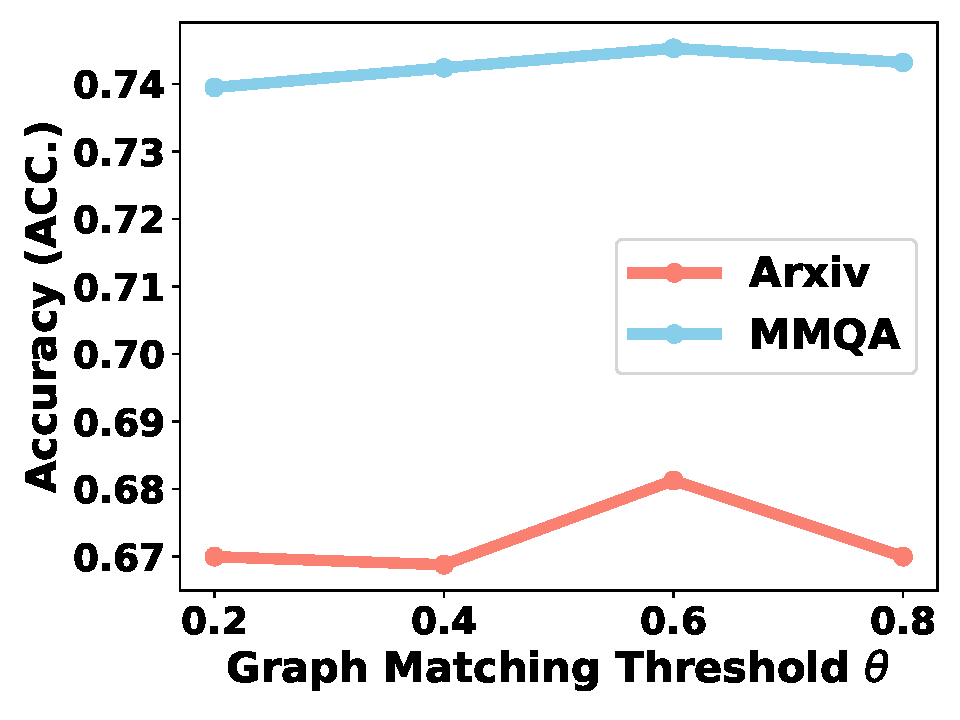
\includegraphics[width=\linewidth]{figures/mgrag/acc_vs_theta_fixed_lp.pdf}
\caption{Similarity threshold $\theta$.}
\end{subfigure}\hfill
\begin{subfigure}{0.48\textwidth}
\centering
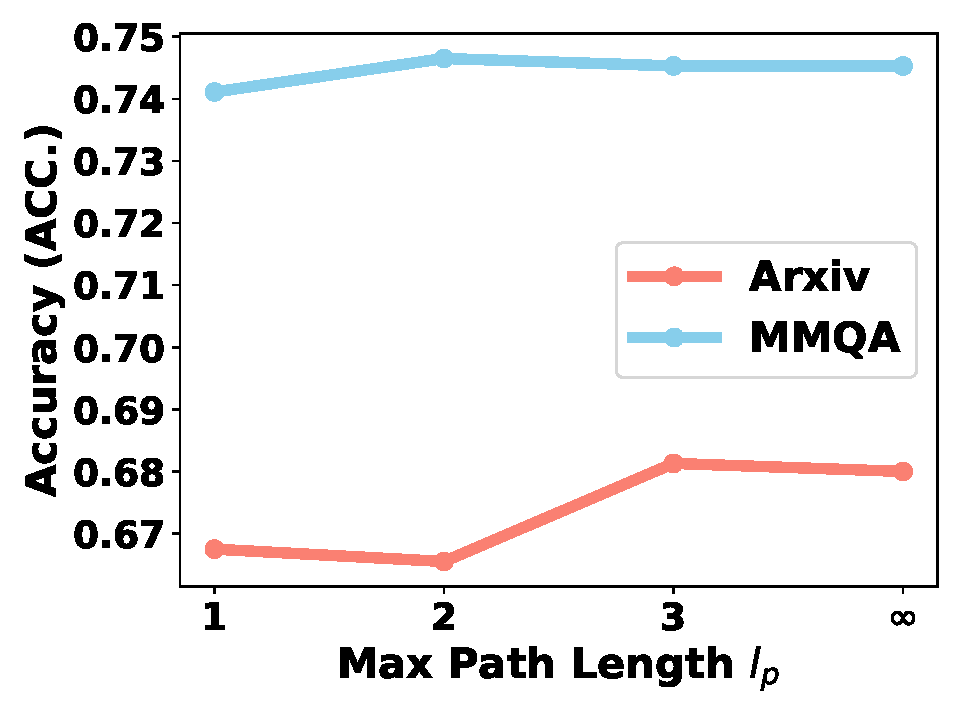
\includegraphics[width=\linewidth]{figures/mgrag/acc_vs_lp_fixed_theta.pdf}
\caption{Maximum path length $l_p$.}
\end{subfigure}
\caption{MGRAG matching-parameter sensitivity. Original subfigures of Figure 5, p.~2491~\cite{mgrag-paper}.}
\label{fig:mgrag:sensitivity}
\end{figure}

The threshold changes which entity correspondences and path extensions can pass validation. A higher value demands closer embedding agreement, while a lower value permits more candidates. The path-length cap determines how many relations may be used to express a query relation. Its effect therefore concerns both representational flexibility and search. These roles explain why the two parameters belong to the matching mechanism, while their empirical choice remains tied to the reported evaluation.

\section{Discussion and Chapter Summary}
\label{sec:mgrag:discussion}

MGRAG gives structure three connected responsibilities. Query-aware extraction determines which facts enter the graph. Path-based matching determines whether those facts express the relational requirements of the query. Graph features then influence the selection of token states for recomputation. The graph is consequently involved in constructing, selecting, and processing evidence, rather than serving only as a store from which a fixed number of items is retrieved.

The experiments support this design at several levels. Complete-system results report the highest values across the seven datasets' four answer metrics. Construction and matching substitutions evaluate the evidence representation and correspondence choices. The hop-group comparison shows additional quality gains for questions requiring more relational steps, together with added time. Cache comparisons and inverse ablations retain the context-serving contribution and expose its dependence on the surrounding retrieval pipeline.

Several conditions delimit the interpretation. Captions influence the coarse order of image evidence, and model-generated extraction determines which facts are available for matching. A valid semantic match is assessed against the extracted query graph and an embedding threshold; answer correctness is evaluated downstream. The maximum construction and path budgets restrict the search. The published runtime measurements use one hardware and model configuration, and the tables do not provide the fixed numerical recomputation budget needed to attribute a cost to a particular $b$ value. These conditions identify the representation and computation choices on which the reported results depend.

For the thesis's central question, the chapter establishes a concrete extension from connected textual evidence to query-dependent multimodal evidence. Semantic paths allow relations to be represented at different granularities across the query and evidence graphs. Selective KV recomputation shows a further use of the retrieved structure in context processing. The following discussion compares these roles with the representations and retrieval objects studied in KGLink, GORAG, and AGRAG, using their respective tasks and published evidence.

\chapter{Discussion}
\label{ch:discussion}

Our research progressed from knowledge-enriched representations to graph construction from task data and prediction without model fine-tuning. Extending retrieval beyond classification introduced requirements for evidence coverage, multimodal correspondence, and context-processing efficiency. This chapter discusses how these requirements shape the construction and use of knowledge structures.

\section{From Knowledge Enrichment to Task-driven Retrieval}
\label{sec:discussion:pipeline}
KGLink uses the semantic information already represented in an external knowledge graph. Graph processing filters linked entities and selects candidate types and feature descriptions before the encoder reads the table. Supervised training learns how these descriptions correspond to annotation labels. The method therefore depends on both the coverage of the external graph and the labeled data available for learning the annotation vocabulary.

GORAG changes the source of the structure and the way the system adapts. Support examples supply keyword--label associations, and later observations expand the index. A large language model uses retrieved labels and their descriptions for classification without task-specific parameter updates. New knowledge enters the graph, allowing the system to incorporate evolving labels and vocabulary without relying on a predefined external knowledge graph.

The required retrieval output becomes richer when moving from classification to generation. Candidate labels constrain a classification decision, while an answer can require several facts and their explanations. AGRAG selects connected facts from a reusable corpus graph and adds source passages to improve information coverage. This makes both the relationships among facts and their original context available to the generator.

\begin{samepage}
For multimodal retrieval, MGRAG addresses the additional need to select and match evidence for each question. The question determines which details to extract from text and images, and semantic matching checks whether evidence paths express the requested relations. Matching controls whether another chunk is processed, while graph features guide the recomputation of cached token states for answering.\par
\end{samepage}

\begin{table}[tbp]
\centering\small
\caption{The roles of structure across the four studies. The entries summarize the methods in their respective research chapters.}
\label{tab:discussion:roles}
\begin{tabular}{>{\raggedright\arraybackslash}p{0.12\textwidth}>{\raggedright\arraybackslash}p{0.24\textwidth}>{\raggedright\arraybackslash}p{0.27\textwidth}>{\raggedright\arraybackslash}p{0.25\textwidth}}
\toprule
Study & Structure source & Selected or represented evidence & Model role\\
\midrule
KGLink & Existing knowledge graph and table links & Candidate types and graph-derived column features & Fine-tuned table encoding and type prediction\\
GORAG & Labeled examples and prescribed online updates & Connected keyword--label evidence and candidate labels & Label-description generation and classification\\
AGRAG & Corpus terms, extracted relations, and passage links & Query-conditioned connected subgraph and hybrid passages & Relation extraction, filtering, and generation\\
MGRAG & Query and ranked multimodal chunks & Semantic path matches, original chunks, and graph features & Query-aware extraction, QA, and selective KV recomputation\\
\bottomrule
\end{tabular}
\end{table}

Table~\ref{tab:discussion:roles} summarizes how the representation changes with the output requirements. Graph descriptions enrich column representations, keyword--label connections constrain candidate classes, and fact paths support generated answers. In MGRAG, the structure also allocates computation when the retrieved context is processed.

\section{Static, Online, and Query-dependent Structures}
\label{sec:discussion:adaptation}
The transition away from a predefined knowledge graph introduces a choice about when to construct and update the replacement structure. KGLink reuses an external graph and adapts evidence selection to each table. Its supervised encoder learns how to use the selected descriptions.

GORAG updates a task index as labels and text arrive. Associations from earlier predictions become available to later queries, so classification performance depends on the sequence of index states.

AGRAG prepares the corpus graph once, then changes query anchors, node influence, edge costs, and subgraph selection for each question. This amortizes graph preparation across repeated queries.

MGRAG extracts facts for each query as it consumes ranked chunks. Matching can stop construction before the full list is processed. Query-aware extraction targets the relationships needed by the current question and adds construction and matching costs to query processing.

GORAG's online updates respond to changes in the task's data, while AGRAG's query-conditioned selection responds to different questions over a shared corpus. MGRAG moves query dependence into extraction itself. The choice therefore depends on how often the source data change, how many queries share the corpus, and whether relevant facts can be extracted before the question is known.

\section{Evidence Quality and Computational Cost}
\label{sec:discussion:cost}
The relevant quality criterion follows the task. A column representation must support the expected type label. Classification retrieval must retain the correct candidate label. Generation requires both sufficient answer coverage and support for the claims produced. Cache reuse must preserve answer quality while reducing processing cost.

Table~\ref{tab:discussion:controls} compares the main experimental conditions. KGLink evaluates a trained encoder; the other studies evaluate generative pipelines with different backbones. Shared datasets also have different supervision and update protocols. GORAG's WOS and IFS-Rel experiments accumulate labels and prediction-derived keyword--label associations over rounds, whereas AGRAG indexes one training passage per label for classification.

\begin{table}[tbp]
\centering\small
\caption{Main experimental conditions across the four studies. Hardware denotes the reported local setup; GORAG's IFS-Rel generation uses the GPT-4o service. Full task-specific controls appear in the corresponding research chapters.}
\label{tab:discussion:controls}
\begin{tabular}{>{\raggedright\arraybackslash}p{0.11\textwidth}>{\raggedright\arraybackslash}p{0.26\textwidth}>{\raggedright\arraybackslash}p{0.28\textwidth}>{\raggedright\arraybackslash}p{0.23\textwidth}}
\toprule
Study & Main model and hardware & Supervision and evidence state & Reported outcome\\
\midrule
KGLink & BERT; Tesla V100 & 7:1:2 train/validation/test; external KG; three-run averages & Annotation accuracy and weighted F1 on a percentage scale\\
GORAG & Qwen2.5-7B on CAD/WOS; GPT-4o on IFS-Rel; A100 40 GB & 1/5/10 support texts per label; cumulative labels; prediction-dependent index updates & Exact-label accuracy by round and support size\\
AGRAG & Qwen2.5-14B-Instruct; A100 80 GB & Fixed corpus graph; query-conditioned scores and subgraph; one training passage per label for classification & Task-specific QA assessment/overlap, coverage, faithfulness, and classification metrics\\
MGRAG & Qwen2.5-VL-7B-Instruct; A100 40 GB & Query-specific multimodal graph; semantic matching; selective KV recomputation & Answer quality, TTFT, and complete-system/module costs\\
\bottomrule
\end{tabular}
\end{table}

\begin{samepage}
The assessment rule follows the output being evaluated. GORAG's accuracy requires the predicted class to match the gold label. AGRAG's QA accuracy uses model judgments scored 0, 0.5, or 1, while its classification accuracy uses label correctness. Its source-defined ROUGE-L quantity divides longest-common-subsequence length by generated-answer length. MGRAG reports answer accuracy alongside semantic similarity and lexical overlap.\par
\end{samepage}

The AGRAG ablations show why coverage and faithfulness must be considered together. Without hybrid passages, the generator can produce supported claims while omitting required information. Graph connectivity helps organize facts, while passages preserve context that extraction or subgraph selection can omit.

MGRAG separates evidence retrieval from reuse of its computation. Cache comparisons measure combined retrieval and serving choices. Inverse ablations test additions within one retrieval pipeline, where improved answer quality can require extra runtime.

Graph preparation and query processing contribute to total cost in different ways. KGLink reports preprocessing and model-processing costs for annotation. GORAG measures the resource demands of its evolving index and retrieval. AGRAG separates corpus indexing from querying. MGRAG reports construction, matching, answer-generation, and end-to-end costs.

\section{Information Preservation and Semantic Granularity}
\label{sec:discussion:preservation}
The hyper-relational study in Chapter~\ref{ch:background} supplies another perspective on structural representations. A main triple and its qualifiers express different aspects of a fact. Decomposing that representation can retain some relationships while losing the association that gives them their meaning. The study examines this issue through decomposition methods, qualifier capture, graph reception, and link-prediction results.

A related design question appears in each core chapter. KGLink must translate graph-derived type descriptions into the annotation task's vocabulary. GORAG associates words with labels whose relevance depends on the classification task. AGRAG selects a graph serialization while retaining a passage channel for information absent from that serialization. MGRAG matches relations to paths that can express a corresponding meaning through a different topology. Each method specifies an evidence unit and a way to relate that unit to the task.

A column vector, candidate label, graph fact, path, and source passage preserve different information. Paths expose intermediate relations, while passages and images retain details that may disappear during extraction. Moving between these representations changes what the next stage must infer.

A useful structure must preserve the relationships needed for the task. Connectivity identifies available links, semantic matching checks their correspondence to a query, and supervision determines the required annotation category. The hyper-relational study examines how graph transformation can alter these relationships before prediction.

\section{Error Propagation Across Structural Decisions}
\label{sec:discussion:unit}
Errors propagate differently depending on where structure enters the pipeline. An incorrect KGLink entity link changes the descriptions offered to the encoder for a table. In GORAG, an incorrect predicted label can become an association available to later queries. AGRAG reuses a corpus graph, so an extracted relation can influence several query-specific selections. MGRAG constructs a new graph for each query, but a mistaken accepted match can end construction before later chunks are examined.

Feedback can target these error sources directly. Entity disambiguation can revise cell links, online correction can revise inserted associations, source verification can check extracted relations, and matching diagnosis can inspect entity alignment and path choices. Chapter~\ref{ch:conclusion} develops these directions.

\section{Limitations and Open Questions}
\label{sec:discussion:limitations}
KGLink's knowledge source is limited by external graph coverage, while its supervised predictor learns the label vocabulary represented in training. Its no-linkage analysis examines how the encoder performs when graph evidence is unavailable.

Constructing a graph from task data shifts the coverage problem to the examples and sources supplied to the system. GORAG starts from sparse support data and can retain errors through prediction-derived updates. Longer streams and different patterns of label evolution remain open evaluation settings.

AGRAG and MGRAG rely on relation extraction, and MGRAG also uses captions to rank images. A useful fact must first survive these preparation steps before structural retrieval can select it. Improving extraction coverage and correcting stored relationships are therefore important for extending the methods to new corpora. Model-assessed QA results additionally depend on the evaluator and its assessment rules.

AGRAG's 2-approximation statement concerns the cost of its initial terminal-connecting tree, and MGRAG's threshold condition concerns accepted path similarities.

\chapter{Conclusion and Future Directions}
\label{ch:conclusion}

\section{Conclusion}
\label{sec:conclusion:findings}
This thesis investigated how explicit knowledge structures can organize and select evidence for language models. It developed four methods for table understanding, dynamic classification, connected textual evidence selection, and multimodal query answering. The studies examine structure at different interfaces: as information supplied to a learned representation, as an index for candidate retrieval, as a connected generation context, and as a signal for context computation.

KGLink's component comparisons show benefits from graph-derived evidence and contextual type-representation training. Its no-linkage subset also shows continued annotation through the table encoder when retrieved KG evidence is absent. External descriptions enter a supervised mapping to the annotation vocabulary, with cross-column filtering determining which descriptions are available.

GORAG's offline ablation shows the contribution of expanding the keyword--label index with earlier predictions under its round protocol. Additional support and cumulative label growth have dataset-dependent effects, including non-monotonic results on IFS-Rel. The study makes evidence maintenance part of dynamic classification: current decisions shape associations available to later candidate retrieval.

AGRAG's ablations distinguish answer coverage from support for the claims actually generated. Removing hybrid passages can retain a high faithfulness score while reducing coverage; replacing the expanded subgraph with its initial tree affects tasks differently. Connected graph facts and passage context therefore serve complementary evidence needs in the evaluated generation tasks.

MGRAG's construction and matching comparisons support query-dependent extraction and semantic paths for the evaluated multimodal questions. Its cache comparisons show that the selected graph can also inform token-state recomputation. Component additions improve answer quality with runtime changes that depend on the host pipeline, extending structural evidence use into context processing.

The accompanying hyper-relational knowledge-graph study examined how structural representations preserve fact information. Its qualifier-capture and graph-reception perspectives help explain why the form of a representation matters. Across the thesis, the common design question is which relationships must remain explicit for the downstream task. The published evaluations answer that question through particular methods and protocols, yielding a set of evidence interfaces for language-model augmentation.

\section{Future Directions}
\label{sec:conclusion:future}
\subsection{Feedback for structure maintenance}
A first direction is to connect evidence maintenance with feedback about its use. The current studies select graph information from an external source, update keyword--label associations, prepare a corpus graph, or build a query-specific graph. Feedback could indicate whether a retrieved relationship was relevant, whether its supporting passage was sufficient, or whether a prediction inserted into an index was later corrected. Such feedback would give maintenance a more direct connection to evidence quality.

The evaluation of this direction should preserve the sequence in which feedback becomes available. In an online classifier, a later correction differs from a gold label supplied before prediction. In a retrieval system, the quality of one answer can affect later evidence selection only after its assessment is available. Explicit feedback timing and provenance would permit the study of correction and retention policies without conflating them with additional supervision.

\subsection{Multimodal structure and provenance}
A second direction concerns the quality of multimodal graph representations. Caption-based ranking provides an efficient text interface for images, while query-aware extraction can target details relevant to a question. Both operations influence which visual information becomes available to semantic matching. A useful extension would retain the link from a graph fact to the text span or image region supporting it, together with the extraction conditions.

This would support a more detailed analysis of retrieval errors. A failed match could result from missing visual evidence, an extraction error, an unsuitable relation representation, or a search decision. Distinguishing these stages would help determine which component to improve. It would also make it possible to assess whether a matched path is supported by the source evidence at the granularity used in the answer.

\subsection{Joint retrieval and context computation}
A third direction is to study retrieval and context serving as coupled decisions. Retrieved evidence determines the length, modality, and structural organization of the model's input. The available cached states and the recomputation policy then determine the cost of processing that input. MGRAG provides one point in this design space by using graph features in selective recomputation.

Further work could evaluate how alternative evidence structures affect the quality--latency tradeoff under a fixed serving budget. The comparison would need to separate graph construction, matching, cache reuse, and answer generation, and retain the query workload and hardware conditions. This would connect the semantic value of retrieved evidence to the cost of using it, extending the thesis's focus on structure from context selection to the complete evidence-processing path.

\printbibliography[heading=bibintoc,title=References]
\end{document}
